\documentclass[11pt,a4paper]{article}
\RequirePackage{amsmath,amssymb,amsfonts,verbatim,graphicx}
\RequirePackage[left=1in,right=1in,top=1in,bottom=1in]{geometry}
\usepackage{xspace,amscd,rotating,latexsym,multicol,array,algorithm,subfigure}
\usepackage[hyphens,obeyspaces]{url}
\usepackage{xcolor}
\usepackage{verbatim} % for commenting out blocks with \begin{comment} \end{comment}
\usepackage{placeins} % for \FloatBarrier

\usepackage{setspace}
\doublespacing

\usepackage{lineno}
\linenumbers

\usepackage[round,authoryear]{natbib}
%\usepackage[
%backend=biber,
%style=authoryear,
%sorting=nyt,
%citestyle=authoryear-comp,
%maxcitenames=2,
%maxbibnames=7,
%minbibnames=7,
%date=year,
%dashed=false,
%natbib=true
%]{biblatex}
%\addbibresource{references.bib}
% make et al. italic
%\usepackage{xpatch}
%\xpatchbibmacro{name:andothers}{%
%  \bibstring{andothers}%
%}{%
%  \bibstring[\emph]{andothers}%
%}{}{}
% comma after author
%\renewcommand*{\nameyeardelim}{\addcomma\space}

\usepackage[hidelinks]{hyperref}
\hypersetup{
    colorlinks=false
}

\pagenumbering{arabic}
\begin{document}

%\input{response}

\newpage
\linenumbers

\noindent
\large{\textbf{Validation of stock assessments: Is it me or my model talking?}
%For as the eyes of bats are to the blaze of day, so is the reason in our soul to the things which are by nature most evident of all.

\noindent
Laurence T. Kell\textsuperscript{1}, Rishi Sharma\textsuperscript{2}, Toshihide Kitakado\textsuperscript{3}, Henning Winker\textsuperscript{4}, Iago Mosqueira\textsuperscript{5}, Massimiliano Cardinale\textsuperscript{6}, Dan Fu\textsuperscript{7}.

\noindent\newline\textsuperscript{1}Centre for Environmental Policy, Imperial College London, Weeks Building, 16-18 Princes Gardens, London, SW7 1NE, UK.
\noindent\newline\textsuperscript{2}Food and Agricultural Organization, Fishery and Aquaculture Policy and Resources Division, Rome, Lazio, 00153, Italy
\noindent\newline\textsuperscript{3}Department of Marine Biosciences, Tokyo University of Marine Science and Technology, 4-5-7 Konan, Minato, Tokyo, 108-8477, Japan.
\noindent\newline\textsuperscript{4}Joint Research Centre (JRC), European Commission, TP 051, Via Enrico Fermi 2749, 21027 
\noindent\newline\textsuperscript{5}Wageningen Marine Research, Haringkade 1, 1976CP IJmuiden, The Netherlands.
\noindent\newline\textsuperscript{6}Swedish University of Agricultural Sciences, Department of Aquatic Resources, Institute of Marine Research, Lysekil, Sweden.
\noindent\newline\textsuperscript{7} Indian Ocean Tuna Commission, Le Chantier Mall, Po Box 1011, Victoria – Seychelles’


\bigskip
\noindent
\textit{Keywords}:  diagnostics, hindcast, prediction skill, retrospective analysis, stock assessment, validation.

\bigskip
\noindent
Manuscript from \today
\newpage
\abstract{

  The adoption of the Precautionary Approach requires providing advice that is robust to uncertainty. Therefore, when conducting stock assessment alternative model structures and data sets are commonly considered. The primary diagnostics used to compare models are to examine residuals patterns to check goodness-of-fit and to conduct retrospective analysis to check the stability of estimates. However, residual patterns can be removed by adding more parameters than justified by the data,  and retrospective patterns removed by ignoring the data. Therefore, neither alone can be used for validation, which requires assessing whether it is plausible that a system identical to the model generated the data. Therefore, we use hindcasting to estimate prediction skill, a measure of the accuracy of a predicted value unknown by the model relative to its observed value, to explore model misspecification and data conflicts. We compare alternative model structures based on integrated statistical and Bayesian state-space biomass dynamic models using, as an example, Indian Ocean yellowfin tuna.  Validation is not a binary process (i.e. pass or fail) but a continuum; therefore, we discuss the use of prediction skill to identify alternative hypotheses, weight ensemble models  and agree on reference sets of operating models when conducting Management Strategy Evaluation.}
  
\newpage
\section{Introduction}

The adoption of the Precautionary Approach to fisheries management \citep[PA,][]{garcia1996precautionary} requires a formal consideration of uncertainty, which is increasingly addressed by conducting stock assessment using alternative modelling frameworks conditioned on a variety of assumptions and data sets. There are various definitions of stock assessment \citep[e.g.][]{hilborn2003state,cadrin2014stock}; our preference is for ``The description of the characteristics of a 'stock' so that its biological reaction to being exploited can be rationally predicted and the predictions tested" (Sidney Holt pers comm.). The reasoning for this is because it explicitly recognises that the main aim of a stock assessment is to provide the basis for long-term sustainable management.  Stock assessment, therefore, requires making and validating probabilistic estimates of stock status and forecasts of the consequences of different management actions. 

Diagnostic tests are essential for determining the robustness of model outputs used to provide management advice \citep{carvalho2020cookbook}. It can be challenging, however, to use traditional diagnostics based on model residuals and likelihoods such as Akaike’s Information Criteria  \citep[AIC,][]{akaike1998information} to compare models. For example, indices of abundance are a primary contributor to the overall likelihood when fitting stock assessment models to data \citep{whitten2013accounting}, and the sum of squared errors (SSE) between observed and predicted indices in the log-space is used as a fitness measure. SSE is problematic because complex models tend to have many parameters to allow flexibility, resulting in a low SSE due to overfitting by adding more parameters than can be justified by the data. Therefore, criteria such as AIC have been developed to aid in model selection. AIC needs to be performed on models with the same likelihood function and data, which is not the case if different hypotheses are modelled with alternative model structures and data sets. Also, AIC is only a relative measure of models' appropriateness, so additional diagnostic tests are needed. This is of particular importance for stock assessment models where only a single historical data set exists, and the system is not observable. 

Therefore, a standard diagnostic tool in stock assessment to check the stability of estimates is retrospective analysis \citep{hurtado2014looking}. The procedure involves sequentially removing all data from the most recent period (i.e. peeling),  refitting the model, and then comparing terminal year estimates of spawning stock biomass (SSB) and fishing mortality ($F$) to the full model. The diagnostic is widely used worldwide to evaluate model estimates' stability, and in Europe is often the key diagnostic for accepting or rejecting a model \citep{ICES2019}. Retrospective analysis has been extended to include stock forecasts, where the terminal year estimates are projected for assumptions about future catches, recruitment, biological parameters and the vulnerability of the stock to fishing \citep[e.g.][]{brooks2016retrospective}. However, stability and a reduction in variance can be achieved at the expense of bias by shrinking terminal estimates towards recent historical values. However, it is impossible to validate a model if bias is unknown, as is the case for unobservable quantities, such as SSB and F \citep{hodges1992you}. Since in such cases, the simplest way to remove a retrospective pattern is to ignore the data. 

Current literature on the comparison of stock assessment methods primarily focuses on how well models fit past data  \citep[e.g.][]{deroba2014simulation}. Historical performance, however, is no indicator of how well a model may perform in the future, which needs to be evaluated if a model is to provide credible and robust advice. 
%In machine learning while estimating the parameters of a prediction function and testing it on the same data may achieve a perfect fit. It might fail to predict anything useful on unseen data. Therefore, when performing machine learning, the common practice is to hold part of the data back, and then compare model estimates to observed values, i.e. cross-validation. 
While prediction is difficult when it is about the future, it is also a daunting task when it comes to the past \citep{glotin2019prediction}. Therefore, when testing mathematical models in many fields, known or closely estimated values for past events are used to see how well model output match known results \citep{jin2008current, weigel2008can, balmaseda1995decadal}. The comparison of model outputs to observations not used in fitting is referred to as “predictive validation” or “cross-validation”, and when the observations are peeled back from the terminal year, this is known as “hindcasting”. Removing observations allows models to be compared using prediction skill \citep{glickman2000glossary}, A measure of a predictor's accuracy compared to its observed value unknown by the model, using metrics such as correlation, relative error, mean absolute scaled error (MASE), and bias.  A predictor refers to a random value that is not part of the dataset. In comparison, an estimator refers to a model parameter.

Model validation is essential in many fields, e.g. climate and energy modelling \citep{kell2020long}, Since it increases confidence in the outputs of a model, leads to an increase in trust amongst the public, stake and asset-holders and policymakers \citep[][]{saltelli2020five}, and can identify model limitations that should be addressed in future research.
%Therefore, we conducted a hindcast by removing observations, generated pseudo observations, and then compared these to the observations omitted. The procedure is non-parametric and is applicable to any automated model building technique. It can provide important diagnostic information about influential cases in the data set and the stability of the model \citep{michaelsen1987cross}. It can therefore be used to validate models, identify model misspecification, data conflicts, and where models need to be modified or extended.
Therefore, in this paper, we validate models using prediction skill by peeling back observations from the final year in the assessment and making predictions of the removed values using a hindcast procedure. We are not proposing the hindcast and prediction skill as the only diagnostic tool used in stock assessment but as a key tool for the assessment toolbox \citep{carvalho2020cookbook}.


\section{Material and Methods}

 As a worked example, we compare three model families used to assess Indian Ocean yellowfin tuna stock \citep{IOTWPTT21}, namely a full integrated statistical model \citep[SS,][]{methot2013stock}, a deterministic age-structured production model \citep[ASPM,][]{maunder2015contemporary}, and a Bayesian state-space biomass dynamic model \citep[JABBA,][]{winker2018jabba}. Both the SS and ASPM models were based on a seasonal structure with four regions, JABBA in comparison, had an annual time step with no spatial structure. 
 
%We conduct model-based and model-free hindcasts to estimate prediction skill using yellowfin tuna (\textit{Thunnus albacares}), as an example based on the Indian Ocean Tuna Commission's most recent assessment . 

After a model structure is agreed upon, it is crucial to validate the model to assesses whether it is plausible that a system identical to the model generated the data \citep{thygesen2017validation}. The ambition of validation is not to prove that a model is correct, but to check that it can not be falsified with the available data. This a different question from asking if the model is fit for a given purpose, which depends on the model's intended use. For example, to evaluate whether an assessment model is robust despite being misspecified, Management Strategy Evaluation \citep[MSE,][]{punt2007developing} can be conducted. See \cite{sharma2020trfmo} for a review of current practice in the Tuna Regional Fisheries Management Organisations (tRFMOs). Validation is not a binary process, i.e. identifying whether a model is valid or invalid, as there is a continuum between these two extremes. Therefore, a primary objective of validation is not to select a "best assessment" but to identify if models are overfitted and how they can be extended or modified to better describe the dynamics.

Model validation, therefore, serves a complimentary purpose to model selection and hypothesis testing. Model selection searches for the most suitable model within a specified family; hypothesis testing examines how to reduce the model structure, while model validation examines if it should be modified or extended. For models to be valid, they must satisfy four prerequisites \citep{hodges1992you}. Namely, the situation modelled must: i) be observable and measurable; ii) be possible to collect sufficient informative data about it; iii) exhibit constancy of structure in time, and iv) exhibit constancy across variations in conditions not specified in the model.

The first two prerequisites should be straight forward; however, many stock assessments, particularly for highly migratory stocks like yellowfin tuna fished in areas beyond national jurisdiction, rely on fishery-dependent data rather than direct scientific observations. The use of fishery-dependent data is a concern since there is evidence that commercial catch per unit effort (CPUE) is likely to remain high while abundance declines \citep{harley2001catch}.  Prerequisite (iii) ensures that the model has prediction skill for the same conditions under which the validation tests were conducted. Prerequisite (iv) ensures that the model will still be valid under conditions that differ from those in the validation tests.

\subsection{Materials}

Yellowfin tuna supports one of the largest tuna fisheries in the Indian Ocean, with catches currently exceeding 400,000t annually. The stock is harvested by various gears, from small-scale artisanal fisheries to large gill netters, industrial longliners, and purse seiners \citep{fiorellato2019tt}.
There are regional differences in the stock and fisheries (figure \ref{fig:map}), and the western tropical region (region 1) is considered the core area of the stock's distribution.

The majority of data available for assessing the stock is fishery-dependent. These include time series of the total catch, seasonal catch per unit effort (CPUE) based on the long-line fisheries \citep{hoyle2020scaling}, Samples of length compositions, tagging recaptures, and environmental data. CPUE are the primary source of information on abundance and are based on a composite long-line index,  spatially stratified by region, from the main distant water fleets. %\citep{hoyle2018yft}. 

Indices in each region are standardised using generalised linear models that accounted for differences in targeting practices and catchability amongst fleets, based on gear configurations and species composition \citep{hoyle2020scaling}. The reason for this is because tuna long-line fishing strategies have changed over time. %\citep{hampton2005}. 
In the assessment, the CPUE indices across regions were linked by a common catchability coefficient, thus improving the model's ability to estimate regional biomass distribution. This required the calculation of arbitrary regional scaling factors related to a reference fleet's catch rates.%\citep{langley2015yft, fu2018yft}.

The length composition data are considered sufficient to provide reasonable estimates of fishery selectivity and recruitment trends but not stock abundance trends. Regional environmental indices (current and sea temperature) allow seasonal and temporal variations to be incorporated in fish movement estimation. Tag release and recovery data collected from the main phase of the Indian Ocean large-scale tuna tagging programme %[Hallier 2008] 
inform estimates of mortality, abundance, and movement. 


\subsection{Assessment Models}

Model development has focused on the spatial structure to account for differences in regional exploitation patterns, and non-stationarity in selectivity and catchability and seasonal movements have been found to resolve data conflicts \citep{urtizberea2018yft}. 
Although a fully integrated statistical model is used to develop the base case, other models are also used.  These include  an age-structured production model \citep[ASPM-R,][]{maunder2015contemporary} and a Bayesian state-space biomass dynamic model \citep[JABBA,][]{winker2018jabba}. 

Stock Synthesis \citep[SS,][]{methot2013stock} is used to conduct the base case assessment and implements an age and spatially structured model that reflects the complex population and fishery dynamics of the stock. The most recent assessment established a base case as a reference model for diagnostics and scenarios to capture various uncertainties \citep{fu2018yft}. The assessment indicates that the stock has declined substantially since 2012, and spawning stock biomass in 2017 is now estimated to be close to the historical lowest level. The stock is estimated to be overfished, and the IOTC has implemented a rebuilding plan to reduce overall fishing pressure.  

%There has been a recent trend in stock assessment toward the use of integrated analysis that combines several sources of data into a single model by a joint likelihood for the observed data \citep[e.g.][]{doubleday1976least,fournier1982general,maunder2013review}. data sets include records of catches and landings, indices of abundance based on catch per unit (CPUE) or from research surveys, and length and age compositions based on samples. An example of an integrated assessment method is SS that can be configured in multiple ways, allowing for a range of scenarios to be developed to reflect uncertainty.

SS provides a flexible framework for conducting stock assessment and 
\cite{maunder2015contemporary} proposed a deterministic implementation in SS of an age-structured production model (ASPM) as a diagnostic of processes that control the expected dynamics through a production function \citep{carvalho2017can}. Selectivity in ASPM is parameterised based on that estimated by a "full" SS model. The model is then refitted to the abundance indices without the size composition contributing to the likelihood. Recruitment deviations can either be estimated (as in our example) or set to zero. This enables an evaluation of whether the observed catches alone can not explain trends in the index of abundance. If the ASPM can fit the indices of abundance well, then a production function is likely to exist (i.e. the dynamics are driven by density-dependent processes), and the indices provide information about absolute abundance. If the fit is poor, then the expected surplus production and observed catches alone can not explain the indices' trends. This can have several causes, namely the (i) stock dynamics are recruitment-driven, (ii) stock has not yet declined to the point at which catch is a major factor influencing abundance; (iii) indices of relative abundance are not proportional to abundance;  (iv) model is incorrectly specified, or (v) data are biased. While a production function was evident in the fit, the overall fit to the indices of abundance in 3 of the 4 areas was poor, and hence we used recruitment deviates to help capture the trends in abundance by area \cite[see][]{minte2017get}. In this study, we implemented ASPM with estimated recruitment deviates (ASPM-R). 

An alternative to an integrated assessment is to use a biomass dynamic model based on an explicit production function. This requires estimation and fixing of fewer parameters and does not use the length composition. We used the R package JABBA (https://github.com/JABBAmodel/jabba) as it provides a unifying, flexible framework for state-space biomass dynamic modelling, runs quickly, and generates reproducible stock status estimates \citep{winker2018jabba}. 
A Pella Tomlinson production function \citep{pella1969generalized} 
was assumed as this allows the shape of the production function to be varied. Allowing alternative assumptions about productivity, stock status, and reference points to be evaluated. JABBA does not account for spatial dynamics, and in this analysis, priors of production function parameters were based on the SS base case. 

\subsection{Assessment Hypotheses}

The base case is spatially disaggregated into two tropical regions (R1 and R4) and two austral subtropical regions (R2 and R3). The tropics encompass the main year-round fisheries, while the long-line fisheries occur more seasonally in the austral regions \citep{langley2015yft}, Reciprocal movement is assumed to occur between adjacent regions. The base case assumes a quarterly time step to approximate the continuous recruitment and rapid growth seen in the yellowfin stock. The population comprised 28 quarterly age-classes with an assumed unexploited equilibrium initial state in each region. Twenty-five fisheries are defined based on fishing gear, region, time period, fishing mode and vessel type. Fisheries were modelled, allowing flexibility in selectivity (e.g. cubic spline or double normal), whereas long-line selectivity was constrained to be fully selective for the older ages. 

Recruitment occurs in the two equatorial regions with temporal deviates in the regional distribution and is assumed to follow a Beverton and Holt stock-recruitment relationship. %(with a steepness of 0.8 and recruitment standard deviation of 0.6).  
Growth is parameterised using age-specific deviates on the $k$ growth parameter to mimic the non-von Bertalanffy growth of juvenile and adults' near-linear growth. Natural mortality varies by age, with the relative trend in age-specific natural mortality based on Pacific Ocean yellowfin \citep{maunder2012review}. 

%[Maunder, M.N., Aires-da-Silva, A. 2012. A review and evaluation of natural mortality for the assessment and management of yellowfin tuna in the eastern Pacific Ocean. External review of IATTC yellowfin tuna assessment. La Jolla, California. 15-19 October 2012. Document YFT-01-07.]


\subsection{Hindcast}

 Validation requires that the system be observable and measurable. So observations should be used unless model estimates are known to be very close to their true values. For example, when conducting a retrospective analysis, a reduction in mean squared error (a measure of variance) of model estimates can be achieved by shrinkage. However, the bias is difficult to quantify in model-based quantities, and therefore, the absence of retrospective patterns while reassuring is not sufficient for validation. For this reason, validation should be conducted using prediction skill based on observations. Therefore, we used a hindcast procedure where the indices of abundance are sequentially removed from the terminal year, i.e. peeled backwards from the model. In contrast, in a retrospective analysis, all observations for a year are peeled back, which means that quantities can not be predicted for the years peeled back unless additional assumptions are made. 
%When conducting the hindcast it is assumed that modelled variables are observable, processes exhibit constancy of structure in time, including those not specified in the model, and that collection of accurate and sufficient data is possible \citep{hodges1992you}.

The hindcast is a variant of cross-validation where, like retrospective analysis, recent data are removed, and the model refitted with the remaining data. Known values (observations) or well estimated historical values are then compared to model estimates. When observations are used for comparison, this is also referred to as model-free validation \citep{kell2016xval}. In a hindcast, observations are removed from the terminal year and up to n years back, and then the missing observations are predicted by fitting to the remaining data for 1, 2, ... n steps ahead. Observations may be removed by series or fleets to evaluate data conflicts, time blocks to overcome serial correlations, or individually to estimate bias as in the jackknife. No stock forecast or projection needs to be performed, and so there is no need to make assumptions about future parameters as all parameters needed are estimated within the model. The hindcast may be conducted for individual data series or combinations of series and data types, for example, by fleet where both CPUE and length data are removed. This allows data conflicts to be explored. Theoretically, the projection period is to the end of the historical time period \citep{brooks2016retrospective}; However, in practice, a step size of one or several years ahead (the horizon $h$) is chosen for the hindcast when removing observations removed from the model fit. This should reflect the time horizon required for robust management advice, considering typical process stochasticity in fishery population dynamics and observation uncertainty. 
%We  define `retro-period' and `hc-period' as `the period of shrunken data set for retrospective model fitting' and `future time period (i.e. horizons) with a certain projection step (say $S \geq 1$) for hindcasting after retro-period''. 
Assessment cycles are typically for three years in most tuna Regional Fisheries Management Organisations and so a horizon of three years was also used.

In this study, only CPUE observations were removed, catch, and length composition remained in the model. Thus, all model fits had the same terminal year and differed only in the length of the CPUE time series. Therefore, the implemented procedure is similar to a jackknife in that we remove points using a peel and then "predict" missing values as part of the fitting process. Time series of pseudo data (i.e. data that are artificially generated to test a program or procedure) were generated from estimates of vulnerable biomass and catchability ($q$). Prediction residuals ($e$) were then computed as the difference between the predictions and the observations. It is possible to perform the hindcast by peeling other data, e.g. the length or age compositions \citep[see][]{carvalho2020cookbook}.
%Hindcasting was not conducted with the length composition data, as it has been demonstrated that following the length data is often misleading if it conflicts with the abundance data \citep{francis2011data}. In addition, in the case of the Indian Ocean yellowfin assessment length had been down weighted significantly so that they did not conflict with the indices of abundance \citep{fu2018yft}. Keeping the catch data meant that it was not necessary to run a projection as an additional step.

%Finally, \cite{minte2017get} demonstrate for BET in the eastern Pacific following the length data can often lead to model misspecification and discuss the trade off of larger uncertainty due to estimating deviates based on indices rather than being more precise but off scale when using the length data, particularly if other parameters such as the life history of the species is misspecified.

\subsubsection{Relative Error}
 
In a retrospective analysis, Mohn's $\rho$ \citep{mohn1999retrospective}, Is commonly used as a measure of relative error for model-based estimates. We used a variant, where we scaled by the mean, so the metric is not affected by the peel's length or the number of steps ahead.

\begin{equation}
\label{eqn:mohn}
\rho_{M} = \frac{1}{n} \sum_{t=T-n}^{T-1} \frac{\hat{y}_{(1:t),t}-\hat{y}_{(1:T),t}}{\hat{y}_{(1:T),t}} 
\end{equation}

\noindent
where $n$ is the number of time steps that the peel is performed for, $t$ is the time for which the missing value estimates, $T$ is the terminal year in the CPUE series, and $\hat{y}$ denotes a model-based quantity, which in this case was $SSB$. The value with suffix $\hat{y}_{(1:T)|t}$ means a value estimated at time $t$ from the full series running from time 1 to $T$, and $\hat{y}_{(1:t),t}$ is the value estimated using the data window from 1 to $t (\leq T)$. The data window is only applicable to the CPUE data window, as the catch and length composition data remain unchanged.

$\rho_M$ is an average of the relative differences at the final time of each window and is a measure of relative retrospective `bias' (scale-free) in a statistical sense. The metric tends to be applied not on the log but the original scale because both positive and negative directions are equivalent. $\rho$ can be estimated for different horizons 
\begin{equation}
\label{eqn:mohn2}
\rho_{M} = \frac{1}{n-h+1} \sum_{t=T-n}^{T-h} \frac{\hat{y}_{(1:t)|t+h}-\hat{y}_{(1:T)|t+h}}{\hat{y}_{(1:T)|t+h}} 
\end{equation}

There is no upper limit for reference values that are low relative to the alternative, while in the reverse case, the error cannot exceed 1.0. Therefore, it is usual to use a lower bound of -0.15 and an upper bound of 0.20 to identify acceptable performance for long-lived species \citep{hurtado2014looking} in practice. For values near or equal to 0, e.g. stocks where exploitation or stock size is low, small absolute differences can result in large relative differences.  This may result in assessments being rejected when needed the most, e.g. during the development of recovery plans, when both stock biomass and fishing mortality may be low. 

\subsubsection{Prediction Skill}

Prediction skill compares an observation at time $t$ ($y_t$) to an prediction of that observation made $h$ time steps previously ($\hat{y}_{t|t-h}$). As a metric, we use the mean absolute scaled error (MASE), as it is a robust and easy to interpret statistic \citep{hyndman2006another}. The MASE compares prediction error ($e_t$) for a prediction horizon of $h$ 

\begin{equation}
\label{eqn:err}
 e_t = y_t -\hat{y}_{t|t-h} 
\end{equation}

\noindent 
to a benchmark forecast corresponding to a na\"{i}ve forecast equal to the last observed value. 

\begin{equation} 
\hat{y}_{t|t-h}=y_{t-h}
\end{equation}

\noindent For a peel of $n$ and a horizon of $h$ years

\begin{equation}
\label{eqn:skill}
MASE=\frac{\frac{1}{n+1}\sum_{t=T-n}^{T} \left| y_t - \hat{y}_{t|t-h} \right|}{\frac{1}{n+1+h}\sum_{t=T-n-h}^{T} \left| y_{t} - {y}_{t-h}\ \right|}
%\frac{\frac{1}{n+1} \sum _{t=T-n}^{T}\left|y_t - \hat{y}_{t|t-h}\right|}{
%                  \frac{1}{n+1+h} 
%                  \sum_{t=T-n-h}^{T}\left|{y_{t} - {y}}_{t-h}}\right|} \\
\end{equation}

The MASE has the desirable properties of scale invariance, so it can compare forecasts across data sets with different scales and has predictable behaviour, symmetry, interpretability and asymptotic normality. Unlike relative error, MASE does not skew its distribution even when the observed values are close to zero. It is easy to interpret as a score of 0.5 indicates that the model forecasts are twice as accurate as a na\"{i}ve baseline prediction. The Diebold-Mariano test \citep{diebold1995comparing} for one-step forecasts can also be used to test the statistical significance of the difference between two sets of forecasts, i.e. by comparing the prediction $y_t -\hat{y}_t$ to a random walk $y_t-y_{t-1}$. 

\section{Results}

The 1-step ahead and the 3-step ahead estimates for model-based quantities are presented in figure \ref{fig:retro} and summarised in table \ref{tab:retro-rho}. These show estimates of stock size ($SSB$ for age-based and biomass ($B$) for length-based methods) and exploitation level (fishing mortality ($F$) or harvest rate ($U$)), relative to their maximum sustainable yield ($MSY$) reference points.

No retrospective pattern is seen for ASPM-R, either for the one (figure \ref{fig:retro}) or three-step (figure \ref{fig:retro3}) ahead forecasts. For SS, a negative bias is seen in $SSB/SSB_{MSY}$ for 1-step ahead, while for 3-steps ahead, $SSB$ is overestimated in the recent period little change is seen in the estimates of $F/F_{MSY}$. JABBA shows a negative pattern for harvest rate, which increases for 3-step ahead forecast. In the case of JABBA although exploitation is less than the ${MSY}$ level stock biomass still declines below $B_{MSY}$, which implies that process error is driving the dynamics. When considering retrospective patterns, $\rho$ has to be in the range $[-0.15,0.2]$ for an assessment to be accepted \citep{ICES2019}. For the 1-step ahead, all the assessments apart from the SS estimates of $F$ pass this test. When the 3-year projection is considered, however, only ASPM-R shows acceptable performance. 

The results from the model-free hindcasts (based on CPUE) are shown in Figures~\ref{fig:hy} and \ref{fig:hy3}for the one and three year ahead predictions respectively; the background colour indicates whether MASE $\le 1$. Table \ref{tab:mase} summarises the MASE values. For SS and JABBA, prediction skill is poor for CPUE indices 2 and 4, while the ASPM-R performs poorly for Region 2. Prediction skill deteriorates for the three-step ahead projections, particularly for SS and JABBA; although for ASPM-R, CPUE indices for Regions 1 and 3 still have good prediction skill. 

The model and prediction residuals for future periods from 1 to 5 steps ahead are summarised in Figure  \ref{fig:residuals} pooling across all CPUE indices. SS becomes increasingly imprecise and biased as the prediction horizon is increased. Although JABBA is more precise, it is still biased.

\section{Discussion}

Of the three structurally different model families used to assess Indian Ocean yellowfin, it was found that the model with the best prediction skill was the ASPM-R. Despite integrating all the available data, the SS base case assessment's poor performance is likely due to large sampling error in the length compositions, introducing noise rather than information about year-class strength. This was confirmed by an additional run performed as a check where the length data were down-weighted (effective sample size was  0.00005), where results were very similar to those of the ASPM-R. 

Results for the ASPM-R suggest that a deterministic age-structured surplus production and observed catches could explain the trends in the indices of abundance and that the base case assessment model is incorrectly specified as it assigns too much weight to spurious signals in the length composition data. The Bayesian state-space biomass dynamic model, by contrast, produced reasonable performance metrics for the core fishing area (Region 1) and the south-western Indian Ocean (Region 3), but could not predict the diverging trends in CPUE for the Eastern Indian Ocean (Regions 3 and 4). Therefore, it appears that it is important for this stock to model both the age structure and spatial dynamics, while the quality of length samples needs to be improved. 

There are many aspects of resource dynamics and productivity about which there is little information in stock assessment data sets \citep[e.g.][]{lee2011m,lee2012steepness, jiao2012modelling,simon2012effects,mangel2013perspective,pepin2015reconsidering,cury2014resolving}. Therefore hypotheses about different plausible states of nature are increasingly represented by alternative model structures, fixed parameters, and weighting of data components \citep[][]{sharma2020trfmo}. Thus, as well as methods for identifying uncertainties and agreeing on scenarios \citep{leach2014elicit}, There is a need for methods to weigh, reject, extend models to include alternative hypotheses, and evaluate the value-of-information associated with different data sets. 

However, model selection based on methods like AIC is only suitable for comparing frameworks based on the same input data. There is also a danger, with diagnostics based on the inspection of residuals, of "hypothesis fishing" or "p-hacking" \citep{wasserstein2016asa,head2015extent}, i.e. finding a pretext for excluding an index or adding extra parameters to improve the fit. On the other hand, if multiple true hypotheses are tested, some will likely be rejected falsely. Thus, it is valuable to reserve part of the data for hindcasting based on model-free validation so that a pattern’s significance is not tested on the same data set that suggested the pattern \citep{arlot2010survey}.

The accuracy and precision of projections depend on the information in the data and determine how far ahead we can predict and the model's potential uses. If a model can not be validated, other uses include using a model as part of a feedback management system and scenario modelling when conducting Management Strategy Evaluation (MSE). An example of a model that can not be validated is a catch only model where if catch observations are removed can not be run. However, it can be simulation tested as part of an MP since feedback means that there is no need for prediction skill.


For example, backtesting is a form of hindcasting used in financial risk modelling to assess a trading or investment strategy's performance. This requires simulating past conditions, which is simple with the hindcast. MSE can be conducted as part of the backtest to allow the impact of feedback on historical catches and stock status to be evaluated. Although it is possible to find a strategy that would have worked well in the past, this is no guarantee that it will work well in the future. Therefore, although a backtest MSE is useful, particularly as it allows stakeholders to see the consequences of a different strategy, it is not sufficient to ensure the robustness of candidate future strategies. Despite this limitation, backtesting may provide insights that are unavailable when models and strategies are tested on simulated data alone.

Another promising field of applications is to use skill-based weighting for multi-model ensembles. A prediction skill score can be used to assign more weight to the better performing models objectively and has been found to improve forecasts \citep[e.g.][]{casanova2009weighting}. %This can be done to weight estimates of current status relative to reference points, or weight Operating Models when conducting MSE. Testing the first approach on an actual case study first was informative as it provides the insight necessary to set up a study on synthetic data.

\section{Conclusions}

The hindcast is an important tool to achieve the aim of this paper, which was to support the definition of stock assessment "as the description of the characteristics of a ’stock’ so that its biological reaction to being exploited can be rationally predicted and the predictions tested." If a model is to be used for forecasting, a model should be validated by comparing predictions to a system's observable and measurable properties \citep{ianelli2016multi}. 

The objective of validation is not to prove that a model is correct, but to check that the model can not be falsified with the available data. In other words, if a model has low prediction skill, then you either need more informative data or to develop alternative models. This is a step forward from hypothesis testing and model selection which is a way of rejecting rather than extending models. 

%The hindcast allows objective comparisons to be made between models with different structures and data sets. This is challenging to do with conventional diagnostics based on likelihoods and model residuals. 
Retrospective analysis evaluates the temporal stability of advice by using a reference series of model estimates based on the most recent assessment. In the Northeast US, allowing for time-varying dynamics (e.g., in natural mortality or catchability) has been used to eliminate retrospective patterns.  This runs the risk of overfitting and could conceivably make estimates more biased \citep{brooks2016retrospective}. It is not possible, however, to estimate bias using model-based and thus latent quantities. Instead, model predictions need to be compared to observations. Therefore, we used the hindcast to calculate prediction skill using simulated observations to identify overfitting and explore how models can be improved based on alternative structural assumptions without the risk of ‘hypothesis fishing’. 

An aim of stock assessment modelling is often to identify a `best' model,  ignoring uncertainty about model structure \citep{jardim2020ensemble}. To move beyond the best assessment to a multiple model approach, procedures need to be agreed upon for the initial selection of models and then for rejecting and weighting them. Currently, once a candidate model is agreed upon, rejection is mainly based on goodness of fit and retrospective analysis. However, this could result in over-fitting, while the best way to remove a retrospective pattern is to ignore the data.
 
Prediction skill is an alternative and can be used to develop advice that is robust to uncertainty by weighing alternative models within an ensemble, either when providing estimates of stock status or when conducting MSE. 

As the stock assessment process becomes more complex, e.g. through the increased use of integrated models, ensembles of models, and MSE, there are concerns about a lack of transparency. This is because of the many internal, implicit, and often poorly documented assumptions and a lack of access as only a few highly skilled experts can run or interrogate the models \citep{hilborn2003state}. Therefore to increase confidence in the outputs of a model and trust amongst the public, stake and asset-holders and policymakers, modellers need to ask, “is it me or my model talking” before others ask the question posed by \cite{hodges1992you} "is it you or your model talking?".

\section{Acknowledgements}

We want to acknowledge Sidney Holt, as it was his comments in the plenary at the World Conference on Stock Assessment Methods in Boston, USA, in 2013 and subsequent email discussions that made us realise that the definition of stock assessment commonly used was inadequate. When we asked him for a definition of stock assessment, this was his reply.

"Your question deserves a serious answer, of course, and it's not easy. I used the term stock assessment because that is one being used loosely in ICES and other places - several terms are these days being used too loosely by scientists - one is 'forage fish'. I now intend to use stock assessment only in a narrow literal sense. To me, it means something like describing the characteristics of a 'stock' in such a way that its biological reaction to being exploited can be rationally predicted and the predictions tested."

This work was carried out using data provided by the International Commission for the Indian  Ocean  Tuna  Commission  (stock assessment)  and reflects the information provided by several IOTC CPCs and the IOTC Secretariat.  This paper's contents do not necessarily reflect the point of view of IOTC and in no way anticipate the Commission's future policy in this area.

We want to thank the ABNJ process in FAO (in particular, Alejandro Anganuzzi) for funding the original meetings across tRFMOs to discuss issues relevant to these assessments. 

\newpage\clearpage
\bibliography{references.bib}
\bibliographystyle{abbrvnat}
%\documentclass[11pt,a4paper]{article}
\RequirePackage{amsmath,amssymb,amsfonts,verbatim,graphicx}
\RequirePackage[left=1in,right=1in,top=1in,bottom=1in]{geometry}
\usepackage{xspace,amscd,rotating,latexsym,multicol,array,algorithm,subfigure}
\usepackage[hyphens,obeyspaces]{url}
\usepackage{xcolor}
\usepackage{verbatim} % for commenting out blocks with \begin{comment} \end{comment}
\usepackage{placeins} % for \FloatBarrier

\usepackage{setspace}
\doublespacing

\usepackage{lineno}
\linenumbers

\usepackage[round,authoryear]{natbib}
%\usepackage[
%backend=biber,
%style=authoryear,
%sorting=nyt,
%citestyle=authoryear-comp,
%maxcitenames=2,
%maxbibnames=7,
%minbibnames=7,
%date=year,
%dashed=false,
%natbib=true
%]{biblatex}
%\addbibresource{references.bib}
% make et al. italic
%\usepackage{xpatch}
%\xpatchbibmacro{name:andothers}{%
%  \bibstring{andothers}%
%}{%
%  \bibstring[\emph]{andothers}%
%}{}{}
% comma after author
%\renewcommand*{\nameyeardelim}{\addcomma\space}

\usepackage[hidelinks]{hyperref}
\hypersetup{
    colorlinks=false
}

\pagenumbering{arabic}
\begin{document}

%\input{response}

\newpage
\linenumbers

\noindent
\large{\textbf{Validation of stock assessments: Is it me or my model talking?}
%For as the eyes of bats are to the blaze of day, so is the reason in our soul to the things which are by nature most evident of all.

\noindent
Laurence T. Kell\textsuperscript{1}, Rishi Sharma\textsuperscript{2}, Toshihide Kitakado\textsuperscript{3}, Henning Winker\textsuperscript{4}, Iago Mosqueira\textsuperscript{5}, Massimiliano Cardinale\textsuperscript{6}, Dan Fu\textsuperscript{7}.

\noindent\newline\textsuperscript{1}Centre for Environmental Policy, Imperial College London, Weeks Building, 16-18 Princes Gardens, London, SW7 1NE, UK.
\noindent\newline\textsuperscript{2}Food and Agricultural Organization, Fishery and Aquaculture Policy and Resources Division, Rome, Lazio, 00153, Italy
\noindent\newline\textsuperscript{3}Department of Marine Biosciences, Tokyo University of Marine Science and Technology, 4-5-7 Konan, Minato, Tokyo, 108-8477, Japan.
\noindent\newline\textsuperscript{4}Joint Research Centre (JRC), European Commission, TP 051, Via Enrico Fermi 2749, 21027 
\noindent\newline\textsuperscript{5}Wageningen Marine Research, Haringkade 1, 1976CP IJmuiden, The Netherlands.
\noindent\newline\textsuperscript{6}Swedish University of Agricultural Sciences, Department of Aquatic Resources, Institute of Marine Research, Lysekil, Sweden.
\noindent\newline\textsuperscript{7} Indian Ocean Tuna Commission, Le Chantier Mall, Po Box 1011, Victoria – Seychelles’


\bigskip
\noindent
\textit{Keywords}:  diagnostics, hindcast, prediction skill, retrospective analysis, stock assessment, validation.

\bigskip
\noindent
Manuscript from \today
\newpage
\abstract{

  The adoption of the Precautionary Approach requires providing advice that is robust to uncertainty. Therefore, when conducting stock assessment alternative model structures and data sets are commonly considered. The primary diagnostics used to compare models are to examine residuals patterns to check goodness-of-fit and to conduct retrospective analysis to check the stability of estimates. However, residual patterns can be removed by adding more parameters than justified by the data,  and retrospective patterns removed by ignoring the data. Therefore, neither alone can be used for validation, which requires assessing whether it is plausible that a system identical to the model generated the data. Therefore, we use hindcasting to estimate prediction skill, a measure of the accuracy of a predicted value unknown by the model relative to its observed value, to explore model misspecification and data conflicts. We compare alternative model structures based on integrated statistical and Bayesian state-space biomass dynamic models using, as an example, Indian Ocean yellowfin tuna.  Validation is not a binary process (i.e. pass or fail) but a continuum; therefore, we discuss the use of prediction skill to identify alternative hypotheses, weight ensemble models  and agree on reference sets of operating models when conducting Management Strategy Evaluation.}
  
\newpage
\section{Introduction}

The adoption of the Precautionary Approach to fisheries management \citep[PA,][]{garcia1996precautionary} requires a formal consideration of uncertainty, which is increasingly addressed by conducting stock assessment using alternative modelling frameworks conditioned on a variety of assumptions and data sets. There are various definitions of stock assessment \citep[e.g.][]{hilborn2003state,cadrin2014stock}; our preference is for ``The description of the characteristics of a 'stock' so that its biological reaction to being exploited can be rationally predicted and the predictions tested" (Sidney Holt pers comm.). The reasoning for this is because it explicitly recognises that the main aim of a stock assessment is to provide the basis for long-term sustainable management.  Stock assessment, therefore, requires making and validating probabilistic estimates of stock status and forecasts of the consequences of different management actions. 

Diagnostic tests are essential for determining the robustness of model outputs used to provide management advice \citep{carvalho2020cookbook}. It can be challenging, however, to use traditional diagnostics based on model residuals and likelihoods such as Akaike’s Information Criteria  \citep[AIC,][]{akaike1998information} to compare models. For example, indices of abundance are a primary contributor to the overall likelihood when fitting stock assessment models to data \citep{whitten2013accounting}, and the sum of squared errors (SSE) between observed and predicted indices in the log-space is used as a fitness measure. SSE is problematic because complex models tend to have many parameters to allow flexibility, resulting in a low SSE due to overfitting by adding more parameters than can be justified by the data. Therefore, criteria such as AIC have been developed to aid in model selection. AIC needs to be performed on models with the same likelihood function and data, which is not the case if different hypotheses are modelled with alternative model structures and data sets. Also, AIC is only a relative measure of models' appropriateness, so additional diagnostic tests are needed. This is of particular importance for stock assessment models where only a single historical data set exists, and the system is not observable. 

Therefore, a standard diagnostic tool in stock assessment to check the stability of estimates is retrospective analysis \citep{hurtado2014looking}. The procedure involves sequentially removing all data from the most recent period (i.e. peeling),  refitting the model, and then comparing terminal year estimates of spawning stock biomass (SSB) and fishing mortality ($F$) to the full model. The diagnostic is widely used worldwide to evaluate model estimates' stability, and in Europe is often the key diagnostic for accepting or rejecting a model \citep{ICES2019}. Retrospective analysis has been extended to include stock forecasts, where the terminal year estimates are projected for assumptions about future catches, recruitment, biological parameters and the vulnerability of the stock to fishing \citep[e.g.][]{brooks2016retrospective}. However, stability and a reduction in variance can be achieved at the expense of bias by shrinking terminal estimates towards recent historical values. However, it is impossible to validate a model if bias is unknown, as is the case for unobservable quantities, such as SSB and F \citep{hodges1992you}. Since in such cases, the simplest way to remove a retrospective pattern is to ignore the data. 

Current literature on the comparison of stock assessment methods primarily focuses on how well models fit past data  \citep[e.g.][]{deroba2014simulation}. Historical performance, however, is no indicator of how well a model may perform in the future, which needs to be evaluated if a model is to provide credible and robust advice. 
%In machine learning while estimating the parameters of a prediction function and testing it on the same data may achieve a perfect fit. It might fail to predict anything useful on unseen data. Therefore, when performing machine learning, the common practice is to hold part of the data back, and then compare model estimates to observed values, i.e. cross-validation. 
While prediction is difficult when it is about the future, it is also a daunting task when it comes to the past \citep{glotin2019prediction}. Therefore, when testing mathematical models in many fields, known or closely estimated values for past events are used to see how well model output match known results \citep{jin2008current, weigel2008can, balmaseda1995decadal}. The comparison of model outputs to observations not used in fitting is referred to as “predictive validation” or “cross-validation”, and when the observations are peeled back from the terminal year, this is known as “hindcasting”. Removing observations allows models to be compared using prediction skill \citep{glickman2000glossary}, A measure of a predictor's accuracy compared to its observed value unknown by the model, using metrics such as correlation, relative error, mean absolute scaled error (MASE), and bias.  A predictor refers to a random value that is not part of the dataset. In comparison, an estimator refers to a model parameter.

Model validation is essential in many fields, e.g. climate and energy modelling \citep{kell2020long}, Since it increases confidence in the outputs of a model, leads to an increase in trust amongst the public, stake and asset-holders and policymakers \citep[][]{saltelli2020five}, and can identify model limitations that should be addressed in future research.
%Therefore, we conducted a hindcast by removing observations, generated pseudo observations, and then compared these to the observations omitted. The procedure is non-parametric and is applicable to any automated model building technique. It can provide important diagnostic information about influential cases in the data set and the stability of the model \citep{michaelsen1987cross}. It can therefore be used to validate models, identify model misspecification, data conflicts, and where models need to be modified or extended.
Therefore, in this paper, we validate models using prediction skill by peeling back observations from the final year in the assessment and making predictions of the removed values using a hindcast procedure. We are not proposing the hindcast and prediction skill as the only diagnostic tool used in stock assessment but as a key tool for the assessment toolbox \citep{carvalho2020cookbook}.


\section{Material and Methods}

 As a worked example, we compare three model families used to assess Indian Ocean yellowfin tuna stock \citep{IOTWPTT21}, namely a full integrated statistical model \citep[SS,][]{methot2013stock}, a deterministic age-structured production model \citep[ASPM,][]{maunder2015contemporary}, and a Bayesian state-space biomass dynamic model \citep[JABBA,][]{winker2018jabba}. Both the SS and ASPM models were based on a seasonal structure with four regions, JABBA in comparison, had an annual time step with no spatial structure. 
 
%We conduct model-based and model-free hindcasts to estimate prediction skill using yellowfin tuna (\textit{Thunnus albacares}), as an example based on the Indian Ocean Tuna Commission's most recent assessment . 

After a model structure is agreed upon, it is crucial to validate the model to assesses whether it is plausible that a system identical to the model generated the data \citep{thygesen2017validation}. The ambition of validation is not to prove that a model is correct, but to check that it can not be falsified with the available data. This a different question from asking if the model is fit for a given purpose, which depends on the model's intended use. For example, to evaluate whether an assessment model is robust despite being misspecified, Management Strategy Evaluation \citep[MSE,][]{punt2007developing} can be conducted. See \cite{sharma2020trfmo} for a review of current practice in the Tuna Regional Fisheries Management Organisations (tRFMOs). Validation is not a binary process, i.e. identifying whether a model is valid or invalid, as there is a continuum between these two extremes. Therefore, a primary objective of validation is not to select a "best assessment" but to identify if models are overfitted and how they can be extended or modified to better describe the dynamics.

Model validation, therefore, serves a complimentary purpose to model selection and hypothesis testing. Model selection searches for the most suitable model within a specified family; hypothesis testing examines how to reduce the model structure, while model validation examines if it should be modified or extended. For models to be valid, they must satisfy four prerequisites \citep{hodges1992you}. Namely, the situation modelled must: i) be observable and measurable; ii) be possible to collect sufficient informative data about it; iii) exhibit constancy of structure in time, and iv) exhibit constancy across variations in conditions not specified in the model.

The first two prerequisites should be straight forward; however, many stock assessments, particularly for highly migratory stocks like yellowfin tuna fished in areas beyond national jurisdiction, rely on fishery-dependent data rather than direct scientific observations. The use of fishery-dependent data is a concern since there is evidence that commercial catch per unit effort (CPUE) is likely to remain high while abundance declines \citep{harley2001catch}.  Prerequisite (iii) ensures that the model has prediction skill for the same conditions under which the validation tests were conducted. Prerequisite (iv) ensures that the model will still be valid under conditions that differ from those in the validation tests.

\subsection{Materials}

Yellowfin tuna supports one of the largest tuna fisheries in the Indian Ocean, with catches currently exceeding 400,000t annually. The stock is harvested by various gears, from small-scale artisanal fisheries to large gill netters, industrial longliners, and purse seiners \citep{fiorellato2019tt}.
There are regional differences in the stock and fisheries (figure \ref{fig:map}), and the western tropical region (region 1) is considered the core area of the stock's distribution.

The majority of data available for assessing the stock is fishery-dependent. These include time series of the total catch, seasonal catch per unit effort (CPUE) based on the long-line fisheries \citep{hoyle2020scaling}, Samples of length compositions, tagging recaptures, and environmental data. CPUE are the primary source of information on abundance and are based on a composite long-line index,  spatially stratified by region, from the main distant water fleets. %\citep{hoyle2018yft}. 

Indices in each region are standardised using generalised linear models that accounted for differences in targeting practices and catchability amongst fleets, based on gear configurations and species composition \citep{hoyle2020scaling}. The reason for this is because tuna long-line fishing strategies have changed over time. %\citep{hampton2005}. 
In the assessment, the CPUE indices across regions were linked by a common catchability coefficient, thus improving the model's ability to estimate regional biomass distribution. This required the calculation of arbitrary regional scaling factors related to a reference fleet's catch rates.%\citep{langley2015yft, fu2018yft}.

The length composition data are considered sufficient to provide reasonable estimates of fishery selectivity and recruitment trends but not stock abundance trends. Regional environmental indices (current and sea temperature) allow seasonal and temporal variations to be incorporated in fish movement estimation. Tag release and recovery data collected from the main phase of the Indian Ocean large-scale tuna tagging programme %[Hallier 2008] 
inform estimates of mortality, abundance, and movement. 


\subsection{Assessment Models}

Model development has focused on the spatial structure to account for differences in regional exploitation patterns, and non-stationarity in selectivity and catchability and seasonal movements have been found to resolve data conflicts \citep{urtizberea2018yft}. 
Although a fully integrated statistical model is used to develop the base case, other models are also used.  These include  an age-structured production model \citep[ASPM-R,][]{maunder2015contemporary} and a Bayesian state-space biomass dynamic model \citep[JABBA,][]{winker2018jabba}. 

Stock Synthesis \citep[SS,][]{methot2013stock} is used to conduct the base case assessment and implements an age and spatially structured model that reflects the complex population and fishery dynamics of the stock. The most recent assessment established a base case as a reference model for diagnostics and scenarios to capture various uncertainties \citep{fu2018yft}. The assessment indicates that the stock has declined substantially since 2012, and spawning stock biomass in 2017 is now estimated to be close to the historical lowest level. The stock is estimated to be overfished, and the IOTC has implemented a rebuilding plan to reduce overall fishing pressure.  

%There has been a recent trend in stock assessment toward the use of integrated analysis that combines several sources of data into a single model by a joint likelihood for the observed data \citep[e.g.][]{doubleday1976least,fournier1982general,maunder2013review}. data sets include records of catches and landings, indices of abundance based on catch per unit (CPUE) or from research surveys, and length and age compositions based on samples. An example of an integrated assessment method is SS that can be configured in multiple ways, allowing for a range of scenarios to be developed to reflect uncertainty.

SS provides a flexible framework for conducting stock assessment and 
\cite{maunder2015contemporary} proposed a deterministic implementation in SS of an age-structured production model (ASPM) as a diagnostic of processes that control the expected dynamics through a production function \citep{carvalho2017can}. Selectivity in ASPM is parameterised based on that estimated by a "full" SS model. The model is then refitted to the abundance indices without the size composition contributing to the likelihood. Recruitment deviations can either be estimated (as in our example) or set to zero. This enables an evaluation of whether the observed catches alone can not explain trends in the index of abundance. If the ASPM can fit the indices of abundance well, then a production function is likely to exist (i.e. the dynamics are driven by density-dependent processes), and the indices provide information about absolute abundance. If the fit is poor, then the expected surplus production and observed catches alone can not explain the indices' trends. This can have several causes, namely the (i) stock dynamics are recruitment-driven, (ii) stock has not yet declined to the point at which catch is a major factor influencing abundance; (iii) indices of relative abundance are not proportional to abundance;  (iv) model is incorrectly specified, or (v) data are biased. While a production function was evident in the fit, the overall fit to the indices of abundance in 3 of the 4 areas was poor, and hence we used recruitment deviates to help capture the trends in abundance by area \cite[see][]{minte2017get}. In this study, we implemented ASPM with estimated recruitment deviates (ASPM-R). 

An alternative to an integrated assessment is to use a biomass dynamic model based on an explicit production function. This requires estimation and fixing of fewer parameters and does not use the length composition. We used the R package JABBA (https://github.com/JABBAmodel/jabba) as it provides a unifying, flexible framework for state-space biomass dynamic modelling, runs quickly, and generates reproducible stock status estimates \citep{winker2018jabba}. 
A Pella Tomlinson production function \citep{pella1969generalized} 
was assumed as this allows the shape of the production function to be varied. Allowing alternative assumptions about productivity, stock status, and reference points to be evaluated. JABBA does not account for spatial dynamics, and in this analysis, priors of production function parameters were based on the SS base case. 

\subsection{Assessment Hypotheses}

The base case is spatially disaggregated into two tropical regions (R1 and R4) and two austral subtropical regions (R2 and R3). The tropics encompass the main year-round fisheries, while the long-line fisheries occur more seasonally in the austral regions \citep{langley2015yft}, Reciprocal movement is assumed to occur between adjacent regions. The base case assumes a quarterly time step to approximate the continuous recruitment and rapid growth seen in the yellowfin stock. The population comprised 28 quarterly age-classes with an assumed unexploited equilibrium initial state in each region. Twenty-five fisheries are defined based on fishing gear, region, time period, fishing mode and vessel type. Fisheries were modelled, allowing flexibility in selectivity (e.g. cubic spline or double normal), whereas long-line selectivity was constrained to be fully selective for the older ages. 

Recruitment occurs in the two equatorial regions with temporal deviates in the regional distribution and is assumed to follow a Beverton and Holt stock-recruitment relationship. %(with a steepness of 0.8 and recruitment standard deviation of 0.6).  
Growth is parameterised using age-specific deviates on the $k$ growth parameter to mimic the non-von Bertalanffy growth of juvenile and adults' near-linear growth. Natural mortality varies by age, with the relative trend in age-specific natural mortality based on Pacific Ocean yellowfin \citep{maunder2012review}. 

%[Maunder, M.N., Aires-da-Silva, A. 2012. A review and evaluation of natural mortality for the assessment and management of yellowfin tuna in the eastern Pacific Ocean. External review of IATTC yellowfin tuna assessment. La Jolla, California. 15-19 October 2012. Document YFT-01-07.]


\subsection{Hindcast}

 Validation requires that the system be observable and measurable. So observations should be used unless model estimates are known to be very close to their true values. For example, when conducting a retrospective analysis, a reduction in mean squared error (a measure of variance) of model estimates can be achieved by shrinkage. However, the bias is difficult to quantify in model-based quantities, and therefore, the absence of retrospective patterns while reassuring is not sufficient for validation. For this reason, validation should be conducted using prediction skill based on observations. Therefore, we used a hindcast procedure where the indices of abundance are sequentially removed from the terminal year, i.e. peeled backwards from the model. In contrast, in a retrospective analysis, all observations for a year are peeled back, which means that quantities can not be predicted for the years peeled back unless additional assumptions are made. 
%When conducting the hindcast it is assumed that modelled variables are observable, processes exhibit constancy of structure in time, including those not specified in the model, and that collection of accurate and sufficient data is possible \citep{hodges1992you}.

The hindcast is a variant of cross-validation where, like retrospective analysis, recent data are removed, and the model refitted with the remaining data. Known values (observations) or well estimated historical values are then compared to model estimates. When observations are used for comparison, this is also referred to as model-free validation \citep{kell2016xval}. In a hindcast, observations are removed from the terminal year and up to n years back, and then the missing observations are predicted by fitting to the remaining data for 1, 2, ... n steps ahead. Observations may be removed by series or fleets to evaluate data conflicts, time blocks to overcome serial correlations, or individually to estimate bias as in the jackknife. No stock forecast or projection needs to be performed, and so there is no need to make assumptions about future parameters as all parameters needed are estimated within the model. The hindcast may be conducted for individual data series or combinations of series and data types, for example, by fleet where both CPUE and length data are removed. This allows data conflicts to be explored. Theoretically, the projection period is to the end of the historical time period \citep{brooks2016retrospective}; However, in practice, a step size of one or several years ahead (the horizon $h$) is chosen for the hindcast when removing observations removed from the model fit. This should reflect the time horizon required for robust management advice, considering typical process stochasticity in fishery population dynamics and observation uncertainty. 
%We  define `retro-period' and `hc-period' as `the period of shrunken data set for retrospective model fitting' and `future time period (i.e. horizons) with a certain projection step (say $S \geq 1$) for hindcasting after retro-period''. 
Assessment cycles are typically for three years in most tuna Regional Fisheries Management Organisations and so a horizon of three years was also used.

In this study, only CPUE observations were removed, catch, and length composition remained in the model. Thus, all model fits had the same terminal year and differed only in the length of the CPUE time series. Therefore, the implemented procedure is similar to a jackknife in that we remove points using a peel and then "predict" missing values as part of the fitting process. Time series of pseudo data (i.e. data that are artificially generated to test a program or procedure) were generated from estimates of vulnerable biomass and catchability ($q$). Prediction residuals ($e$) were then computed as the difference between the predictions and the observations. It is possible to perform the hindcast by peeling other data, e.g. the length or age compositions \citep[see][]{carvalho2020cookbook}.
%Hindcasting was not conducted with the length composition data, as it has been demonstrated that following the length data is often misleading if it conflicts with the abundance data \citep{francis2011data}. In addition, in the case of the Indian Ocean yellowfin assessment length had been down weighted significantly so that they did not conflict with the indices of abundance \citep{fu2018yft}. Keeping the catch data meant that it was not necessary to run a projection as an additional step.

%Finally, \cite{minte2017get} demonstrate for BET in the eastern Pacific following the length data can often lead to model misspecification and discuss the trade off of larger uncertainty due to estimating deviates based on indices rather than being more precise but off scale when using the length data, particularly if other parameters such as the life history of the species is misspecified.

\subsubsection{Relative Error}
 
In a retrospective analysis, Mohn's $\rho$ \citep{mohn1999retrospective}, Is commonly used as a measure of relative error for model-based estimates. We used a variant, where we scaled by the mean, so the metric is not affected by the peel's length or the number of steps ahead.

\begin{equation}
\label{eqn:mohn}
\rho_{M} = \frac{1}{n} \sum_{t=T-n}^{T-1} \frac{\hat{y}_{(1:t),t}-\hat{y}_{(1:T),t}}{\hat{y}_{(1:T),t}} 
\end{equation}

\noindent
where $n$ is the number of time steps that the peel is performed for, $t$ is the time for which the missing value estimates, $T$ is the terminal year in the CPUE series, and $\hat{y}$ denotes a model-based quantity, which in this case was $SSB$. The value with suffix $\hat{y}_{(1:T)|t}$ means a value estimated at time $t$ from the full series running from time 1 to $T$, and $\hat{y}_{(1:t),t}$ is the value estimated using the data window from 1 to $t (\leq T)$. The data window is only applicable to the CPUE data window, as the catch and length composition data remain unchanged.

$\rho_M$ is an average of the relative differences at the final time of each window and is a measure of relative retrospective `bias' (scale-free) in a statistical sense. The metric tends to be applied not on the log but the original scale because both positive and negative directions are equivalent. $\rho$ can be estimated for different horizons 
\begin{equation}
\label{eqn:mohn2}
\rho_{M} = \frac{1}{n-h+1} \sum_{t=T-n}^{T-h} \frac{\hat{y}_{(1:t)|t+h}-\hat{y}_{(1:T)|t+h}}{\hat{y}_{(1:T)|t+h}} 
\end{equation}

There is no upper limit for reference values that are low relative to the alternative, while in the reverse case, the error cannot exceed 1.0. Therefore, it is usual to use a lower bound of -0.15 and an upper bound of 0.20 to identify acceptable performance for long-lived species \citep{hurtado2014looking} in practice. For values near or equal to 0, e.g. stocks where exploitation or stock size is low, small absolute differences can result in large relative differences.  This may result in assessments being rejected when needed the most, e.g. during the development of recovery plans, when both stock biomass and fishing mortality may be low. 

\subsubsection{Prediction Skill}

Prediction skill compares an observation at time $t$ ($y_t$) to an prediction of that observation made $h$ time steps previously ($\hat{y}_{t|t-h}$). As a metric, we use the mean absolute scaled error (MASE), as it is a robust and easy to interpret statistic \citep{hyndman2006another}. The MASE compares prediction error ($e_t$) for a prediction horizon of $h$ 

\begin{equation}
\label{eqn:err}
 e_t = y_t -\hat{y}_{t|t-h} 
\end{equation}

\noindent 
to a benchmark forecast corresponding to a na\"{i}ve forecast equal to the last observed value. 

\begin{equation} 
\hat{y}_{t|t-h}=y_{t-h}
\end{equation}

\noindent For a peel of $n$ and a horizon of $h$ years

\begin{equation}
\label{eqn:skill}
MASE=\frac{\frac{1}{n+1}\sum_{t=T-n}^{T} \left| y_t - \hat{y}_{t|t-h} \right|}{\frac{1}{n+1+h}\sum_{t=T-n-h}^{T} \left| y_{t} - {y}_{t-h}\ \right|}
%\frac{\frac{1}{n+1} \sum _{t=T-n}^{T}\left|y_t - \hat{y}_{t|t-h}\right|}{
%                  \frac{1}{n+1+h} 
%                  \sum_{t=T-n-h}^{T}\left|{y_{t} - {y}}_{t-h}}\right|} \\
\end{equation}

The MASE has the desirable properties of scale invariance, so it can compare forecasts across data sets with different scales and has predictable behaviour, symmetry, interpretability and asymptotic normality. Unlike relative error, MASE does not skew its distribution even when the observed values are close to zero. It is easy to interpret as a score of 0.5 indicates that the model forecasts are twice as accurate as a na\"{i}ve baseline prediction. The Diebold-Mariano test \citep{diebold1995comparing} for one-step forecasts can also be used to test the statistical significance of the difference between two sets of forecasts, i.e. by comparing the prediction $y_t -\hat{y}_t$ to a random walk $y_t-y_{t-1}$. 

\section{Results}

The 1-step ahead and the 3-step ahead estimates for model-based quantities are presented in figure \ref{fig:retro} and summarised in table \ref{tab:retro-rho}. These show estimates of stock size ($SSB$ for age-based and biomass ($B$) for length-based methods) and exploitation level (fishing mortality ($F$) or harvest rate ($U$)), relative to their maximum sustainable yield ($MSY$) reference points.

No retrospective pattern is seen for ASPM-R, either for the one (figure \ref{fig:retro}) or three-step (figure \ref{fig:retro3}) ahead forecasts. For SS, a negative bias is seen in $SSB/SSB_{MSY}$ for 1-step ahead, while for 3-steps ahead, $SSB$ is overestimated in the recent period little change is seen in the estimates of $F/F_{MSY}$. JABBA shows a negative pattern for harvest rate, which increases for 3-step ahead forecast. In the case of JABBA although exploitation is less than the ${MSY}$ level stock biomass still declines below $B_{MSY}$, which implies that process error is driving the dynamics. When considering retrospective patterns, $\rho$ has to be in the range $[-0.15,0.2]$ for an assessment to be accepted \citep{ICES2019}. For the 1-step ahead, all the assessments apart from the SS estimates of $F$ pass this test. When the 3-year projection is considered, however, only ASPM-R shows acceptable performance. 

The results from the model-free hindcasts (based on CPUE) are shown in Figures~\ref{fig:hy} and \ref{fig:hy3}for the one and three year ahead predictions respectively; the background colour indicates whether MASE $\le 1$. Table \ref{tab:mase} summarises the MASE values. For SS and JABBA, prediction skill is poor for CPUE indices 2 and 4, while the ASPM-R performs poorly for Region 2. Prediction skill deteriorates for the three-step ahead projections, particularly for SS and JABBA; although for ASPM-R, CPUE indices for Regions 1 and 3 still have good prediction skill. 

The model and prediction residuals for future periods from 1 to 5 steps ahead are summarised in Figure  \ref{fig:residuals} pooling across all CPUE indices. SS becomes increasingly imprecise and biased as the prediction horizon is increased. Although JABBA is more precise, it is still biased.

\section{Discussion}

Of the three structurally different model families used to assess Indian Ocean yellowfin, it was found that the model with the best prediction skill was the ASPM-R. Despite integrating all the available data, the SS base case assessment's poor performance is likely due to large sampling error in the length compositions, introducing noise rather than information about year-class strength. This was confirmed by an additional run performed as a check where the length data were down-weighted (effective sample size was  0.00005), where results were very similar to those of the ASPM-R. 

Results for the ASPM-R suggest that a deterministic age-structured surplus production and observed catches could explain the trends in the indices of abundance and that the base case assessment model is incorrectly specified as it assigns too much weight to spurious signals in the length composition data. The Bayesian state-space biomass dynamic model, by contrast, produced reasonable performance metrics for the core fishing area (Region 1) and the south-western Indian Ocean (Region 3), but could not predict the diverging trends in CPUE for the Eastern Indian Ocean (Regions 3 and 4). Therefore, it appears that it is important for this stock to model both the age structure and spatial dynamics, while the quality of length samples needs to be improved. 

There are many aspects of resource dynamics and productivity about which there is little information in stock assessment data sets \citep[e.g.][]{lee2011m,lee2012steepness, jiao2012modelling,simon2012effects,mangel2013perspective,pepin2015reconsidering,cury2014resolving}. Therefore hypotheses about different plausible states of nature are increasingly represented by alternative model structures, fixed parameters, and weighting of data components \citep[][]{sharma2020trfmo}. Thus, as well as methods for identifying uncertainties and agreeing on scenarios \citep{leach2014elicit}, There is a need for methods to weigh, reject, extend models to include alternative hypotheses, and evaluate the value-of-information associated with different data sets. 

However, model selection based on methods like AIC is only suitable for comparing frameworks based on the same input data. There is also a danger, with diagnostics based on the inspection of residuals, of "hypothesis fishing" or "p-hacking" \citep{wasserstein2016asa,head2015extent}, i.e. finding a pretext for excluding an index or adding extra parameters to improve the fit. On the other hand, if multiple true hypotheses are tested, some will likely be rejected falsely. Thus, it is valuable to reserve part of the data for hindcasting based on model-free validation so that a pattern’s significance is not tested on the same data set that suggested the pattern \citep{arlot2010survey}.

The accuracy and precision of projections depend on the information in the data and determine how far ahead we can predict and the model's potential uses. If a model can not be validated, other uses include using a model as part of a feedback management system and scenario modelling when conducting Management Strategy Evaluation (MSE). An example of a model that can not be validated is a catch only model where if catch observations are removed can not be run. However, it can be simulation tested as part of an MP since feedback means that there is no need for prediction skill.


For example, backtesting is a form of hindcasting used in financial risk modelling to assess a trading or investment strategy's performance. This requires simulating past conditions, which is simple with the hindcast. MSE can be conducted as part of the backtest to allow the impact of feedback on historical catches and stock status to be evaluated. Although it is possible to find a strategy that would have worked well in the past, this is no guarantee that it will work well in the future. Therefore, although a backtest MSE is useful, particularly as it allows stakeholders to see the consequences of a different strategy, it is not sufficient to ensure the robustness of candidate future strategies. Despite this limitation, backtesting may provide insights that are unavailable when models and strategies are tested on simulated data alone.

Another promising field of applications is to use skill-based weighting for multi-model ensembles. A prediction skill score can be used to assign more weight to the better performing models objectively and has been found to improve forecasts \citep[e.g.][]{casanova2009weighting}. %This can be done to weight estimates of current status relative to reference points, or weight Operating Models when conducting MSE. Testing the first approach on an actual case study first was informative as it provides the insight necessary to set up a study on synthetic data.

\section{Conclusions}

The hindcast is an important tool to achieve the aim of this paper, which was to support the definition of stock assessment "as the description of the characteristics of a ’stock’ so that its biological reaction to being exploited can be rationally predicted and the predictions tested." If a model is to be used for forecasting, a model should be validated by comparing predictions to a system's observable and measurable properties \citep{ianelli2016multi}. 

The objective of validation is not to prove that a model is correct, but to check that the model can not be falsified with the available data. In other words, if a model has low prediction skill, then you either need more informative data or to develop alternative models. This is a step forward from hypothesis testing and model selection which is a way of rejecting rather than extending models. 

%The hindcast allows objective comparisons to be made between models with different structures and data sets. This is challenging to do with conventional diagnostics based on likelihoods and model residuals. 
Retrospective analysis evaluates the temporal stability of advice by using a reference series of model estimates based on the most recent assessment. In the Northeast US, allowing for time-varying dynamics (e.g., in natural mortality or catchability) has been used to eliminate retrospective patterns.  This runs the risk of overfitting and could conceivably make estimates more biased \citep{brooks2016retrospective}. It is not possible, however, to estimate bias using model-based and thus latent quantities. Instead, model predictions need to be compared to observations. Therefore, we used the hindcast to calculate prediction skill using simulated observations to identify overfitting and explore how models can be improved based on alternative structural assumptions without the risk of ‘hypothesis fishing’. 

An aim of stock assessment modelling is often to identify a `best' model,  ignoring uncertainty about model structure \citep{jardim2020ensemble}. To move beyond the best assessment to a multiple model approach, procedures need to be agreed upon for the initial selection of models and then for rejecting and weighting them. Currently, once a candidate model is agreed upon, rejection is mainly based on goodness of fit and retrospective analysis. However, this could result in over-fitting, while the best way to remove a retrospective pattern is to ignore the data.
 
Prediction skill is an alternative and can be used to develop advice that is robust to uncertainty by weighing alternative models within an ensemble, either when providing estimates of stock status or when conducting MSE. 

As the stock assessment process becomes more complex, e.g. through the increased use of integrated models, ensembles of models, and MSE, there are concerns about a lack of transparency. This is because of the many internal, implicit, and often poorly documented assumptions and a lack of access as only a few highly skilled experts can run or interrogate the models \citep{hilborn2003state}. Therefore to increase confidence in the outputs of a model and trust amongst the public, stake and asset-holders and policymakers, modellers need to ask, “is it me or my model talking” before others ask the question posed by \cite{hodges1992you} "is it you or your model talking?".

\section{Acknowledgements}

We want to acknowledge Sidney Holt, as it was his comments in the plenary at the World Conference on Stock Assessment Methods in Boston, USA, in 2013 and subsequent email discussions that made us realise that the definition of stock assessment commonly used was inadequate. When we asked him for a definition of stock assessment, this was his reply.

"Your question deserves a serious answer, of course, and it's not easy. I used the term stock assessment because that is one being used loosely in ICES and other places - several terms are these days being used too loosely by scientists - one is 'forage fish'. I now intend to use stock assessment only in a narrow literal sense. To me, it means something like describing the characteristics of a 'stock' in such a way that its biological reaction to being exploited can be rationally predicted and the predictions tested."

This work was carried out using data provided by the International Commission for the Indian  Ocean  Tuna  Commission  (stock assessment)  and reflects the information provided by several IOTC CPCs and the IOTC Secretariat.  This paper's contents do not necessarily reflect the point of view of IOTC and in no way anticipate the Commission's future policy in this area.

We want to thank the ABNJ process in FAO (in particular, Alejandro Anganuzzi) for funding the original meetings across tRFMOs to discuss issues relevant to these assessments. 

\newpage\clearpage
\bibliography{references.bib}
\bibliographystyle{abbrvnat}
%\documentclass[11pt,a4paper]{article}
\RequirePackage{amsmath,amssymb,amsfonts,verbatim,graphicx}
\RequirePackage[left=1in,right=1in,top=1in,bottom=1in]{geometry}
\usepackage{xspace,amscd,rotating,latexsym,multicol,array,algorithm,subfigure}
\usepackage[hyphens,obeyspaces]{url}
\usepackage{xcolor}
\usepackage{verbatim} % for commenting out blocks with \begin{comment} \end{comment}
\usepackage{placeins} % for \FloatBarrier

\usepackage{setspace}
\doublespacing

\usepackage{lineno}
\linenumbers

\usepackage[round,authoryear]{natbib}
%\usepackage[
%backend=biber,
%style=authoryear,
%sorting=nyt,
%citestyle=authoryear-comp,
%maxcitenames=2,
%maxbibnames=7,
%minbibnames=7,
%date=year,
%dashed=false,
%natbib=true
%]{biblatex}
%\addbibresource{references.bib}
% make et al. italic
%\usepackage{xpatch}
%\xpatchbibmacro{name:andothers}{%
%  \bibstring{andothers}%
%}{%
%  \bibstring[\emph]{andothers}%
%}{}{}
% comma after author
%\renewcommand*{\nameyeardelim}{\addcomma\space}

\usepackage[hidelinks]{hyperref}
\hypersetup{
    colorlinks=false
}

\pagenumbering{arabic}
\begin{document}

%\input{response}

\newpage
\linenumbers

\noindent
\large{\textbf{Validation of stock assessments: Is it me or my model talking?}
%For as the eyes of bats are to the blaze of day, so is the reason in our soul to the things which are by nature most evident of all.

\noindent
Laurence T. Kell\textsuperscript{1}, Rishi Sharma\textsuperscript{2}, Toshihide Kitakado\textsuperscript{3}, Henning Winker\textsuperscript{4}, Iago Mosqueira\textsuperscript{5}, Massimiliano Cardinale\textsuperscript{6}, Dan Fu\textsuperscript{7}.

\noindent\newline\textsuperscript{1}Centre for Environmental Policy, Imperial College London, Weeks Building, 16-18 Princes Gardens, London, SW7 1NE, UK.
\noindent\newline\textsuperscript{2}Food and Agricultural Organization, Fishery and Aquaculture Policy and Resources Division, Rome, Lazio, 00153, Italy
\noindent\newline\textsuperscript{3}Department of Marine Biosciences, Tokyo University of Marine Science and Technology, 4-5-7 Konan, Minato, Tokyo, 108-8477, Japan.
\noindent\newline\textsuperscript{4}Joint Research Centre (JRC), European Commission, TP 051, Via Enrico Fermi 2749, 21027 
\noindent\newline\textsuperscript{5}Wageningen Marine Research, Haringkade 1, 1976CP IJmuiden, The Netherlands.
\noindent\newline\textsuperscript{6}Swedish University of Agricultural Sciences, Department of Aquatic Resources, Institute of Marine Research, Lysekil, Sweden.
\noindent\newline\textsuperscript{7} Indian Ocean Tuna Commission, Le Chantier Mall, Po Box 1011, Victoria – Seychelles’


\bigskip
\noindent
\textit{Keywords}:  diagnostics, hindcast, prediction skill, retrospective analysis, stock assessment, validation.

\bigskip
\noindent
Manuscript from \today
\newpage
\abstract{

  The adoption of the Precautionary Approach requires providing advice that is robust to uncertainty. Therefore, when conducting stock assessment alternative model structures and data sets are commonly considered. The primary diagnostics used to compare models are to examine residuals patterns to check goodness-of-fit and to conduct retrospective analysis to check the stability of estimates. However, residual patterns can be removed by adding more parameters than justified by the data,  and retrospective patterns removed by ignoring the data. Therefore, neither alone can be used for validation, which requires assessing whether it is plausible that a system identical to the model generated the data. Therefore, we use hindcasting to estimate prediction skill, a measure of the accuracy of a predicted value unknown by the model relative to its observed value, to explore model misspecification and data conflicts. We compare alternative model structures based on integrated statistical and Bayesian state-space biomass dynamic models using, as an example, Indian Ocean yellowfin tuna.  Validation is not a binary process (i.e. pass or fail) but a continuum; therefore, we discuss the use of prediction skill to identify alternative hypotheses, weight ensemble models  and agree on reference sets of operating models when conducting Management Strategy Evaluation.}
  
\newpage
\section{Introduction}

The adoption of the Precautionary Approach to fisheries management \citep[PA,][]{garcia1996precautionary} requires a formal consideration of uncertainty, which is increasingly addressed by conducting stock assessment using alternative modelling frameworks conditioned on a variety of assumptions and data sets. There are various definitions of stock assessment \citep[e.g.][]{hilborn2003state,cadrin2014stock}; our preference is for ``The description of the characteristics of a 'stock' so that its biological reaction to being exploited can be rationally predicted and the predictions tested" (Sidney Holt pers comm.). The reasoning for this is because it explicitly recognises that the main aim of a stock assessment is to provide the basis for long-term sustainable management.  Stock assessment, therefore, requires making and validating probabilistic estimates of stock status and forecasts of the consequences of different management actions. 

Diagnostic tests are essential for determining the robustness of model outputs used to provide management advice \citep{carvalho2020cookbook}. It can be challenging, however, to use traditional diagnostics based on model residuals and likelihoods such as Akaike’s Information Criteria  \citep[AIC,][]{akaike1998information} to compare models. For example, indices of abundance are a primary contributor to the overall likelihood when fitting stock assessment models to data \citep{whitten2013accounting}, and the sum of squared errors (SSE) between observed and predicted indices in the log-space is used as a fitness measure. SSE is problematic because complex models tend to have many parameters to allow flexibility, resulting in a low SSE due to overfitting by adding more parameters than can be justified by the data. Therefore, criteria such as AIC have been developed to aid in model selection. AIC needs to be performed on models with the same likelihood function and data, which is not the case if different hypotheses are modelled with alternative model structures and data sets. Also, AIC is only a relative measure of models' appropriateness, so additional diagnostic tests are needed. This is of particular importance for stock assessment models where only a single historical data set exists, and the system is not observable. 

Therefore, a standard diagnostic tool in stock assessment to check the stability of estimates is retrospective analysis \citep{hurtado2014looking}. The procedure involves sequentially removing all data from the most recent period (i.e. peeling),  refitting the model, and then comparing terminal year estimates of spawning stock biomass (SSB) and fishing mortality ($F$) to the full model. The diagnostic is widely used worldwide to evaluate model estimates' stability, and in Europe is often the key diagnostic for accepting or rejecting a model \citep{ICES2019}. Retrospective analysis has been extended to include stock forecasts, where the terminal year estimates are projected for assumptions about future catches, recruitment, biological parameters and the vulnerability of the stock to fishing \citep[e.g.][]{brooks2016retrospective}. However, stability and a reduction in variance can be achieved at the expense of bias by shrinking terminal estimates towards recent historical values. However, it is impossible to validate a model if bias is unknown, as is the case for unobservable quantities, such as SSB and F \citep{hodges1992you}. Since in such cases, the simplest way to remove a retrospective pattern is to ignore the data. 

Current literature on the comparison of stock assessment methods primarily focuses on how well models fit past data  \citep[e.g.][]{deroba2014simulation}. Historical performance, however, is no indicator of how well a model may perform in the future, which needs to be evaluated if a model is to provide credible and robust advice. 
%In machine learning while estimating the parameters of a prediction function and testing it on the same data may achieve a perfect fit. It might fail to predict anything useful on unseen data. Therefore, when performing machine learning, the common practice is to hold part of the data back, and then compare model estimates to observed values, i.e. cross-validation. 
While prediction is difficult when it is about the future, it is also a daunting task when it comes to the past \citep{glotin2019prediction}. Therefore, when testing mathematical models in many fields, known or closely estimated values for past events are used to see how well model output match known results \citep{jin2008current, weigel2008can, balmaseda1995decadal}. The comparison of model outputs to observations not used in fitting is referred to as “predictive validation” or “cross-validation”, and when the observations are peeled back from the terminal year, this is known as “hindcasting”. Removing observations allows models to be compared using prediction skill \citep{glickman2000glossary}, A measure of a predictor's accuracy compared to its observed value unknown by the model, using metrics such as correlation, relative error, mean absolute scaled error (MASE), and bias.  A predictor refers to a random value that is not part of the dataset. In comparison, an estimator refers to a model parameter.

Model validation is essential in many fields, e.g. climate and energy modelling \citep{kell2020long}, Since it increases confidence in the outputs of a model, leads to an increase in trust amongst the public, stake and asset-holders and policymakers \citep[][]{saltelli2020five}, and can identify model limitations that should be addressed in future research.
%Therefore, we conducted a hindcast by removing observations, generated pseudo observations, and then compared these to the observations omitted. The procedure is non-parametric and is applicable to any automated model building technique. It can provide important diagnostic information about influential cases in the data set and the stability of the model \citep{michaelsen1987cross}. It can therefore be used to validate models, identify model misspecification, data conflicts, and where models need to be modified or extended.
Therefore, in this paper, we validate models using prediction skill by peeling back observations from the final year in the assessment and making predictions of the removed values using a hindcast procedure. We are not proposing the hindcast and prediction skill as the only diagnostic tool used in stock assessment but as a key tool for the assessment toolbox \citep{carvalho2020cookbook}.


\section{Material and Methods}

 As a worked example, we compare three model families used to assess Indian Ocean yellowfin tuna stock \citep{IOTWPTT21}, namely a full integrated statistical model \citep[SS,][]{methot2013stock}, a deterministic age-structured production model \citep[ASPM,][]{maunder2015contemporary}, and a Bayesian state-space biomass dynamic model \citep[JABBA,][]{winker2018jabba}. Both the SS and ASPM models were based on a seasonal structure with four regions, JABBA in comparison, had an annual time step with no spatial structure. 
 
%We conduct model-based and model-free hindcasts to estimate prediction skill using yellowfin tuna (\textit{Thunnus albacares}), as an example based on the Indian Ocean Tuna Commission's most recent assessment . 

After a model structure is agreed upon, it is crucial to validate the model to assesses whether it is plausible that a system identical to the model generated the data \citep{thygesen2017validation}. The ambition of validation is not to prove that a model is correct, but to check that it can not be falsified with the available data. This a different question from asking if the model is fit for a given purpose, which depends on the model's intended use. For example, to evaluate whether an assessment model is robust despite being misspecified, Management Strategy Evaluation \citep[MSE,][]{punt2007developing} can be conducted. See \cite{sharma2020trfmo} for a review of current practice in the Tuna Regional Fisheries Management Organisations (tRFMOs). Validation is not a binary process, i.e. identifying whether a model is valid or invalid, as there is a continuum between these two extremes. Therefore, a primary objective of validation is not to select a "best assessment" but to identify if models are overfitted and how they can be extended or modified to better describe the dynamics.

Model validation, therefore, serves a complimentary purpose to model selection and hypothesis testing. Model selection searches for the most suitable model within a specified family; hypothesis testing examines how to reduce the model structure, while model validation examines if it should be modified or extended. For models to be valid, they must satisfy four prerequisites \citep{hodges1992you}. Namely, the situation modelled must: i) be observable and measurable; ii) be possible to collect sufficient informative data about it; iii) exhibit constancy of structure in time, and iv) exhibit constancy across variations in conditions not specified in the model.

The first two prerequisites should be straight forward; however, many stock assessments, particularly for highly migratory stocks like yellowfin tuna fished in areas beyond national jurisdiction, rely on fishery-dependent data rather than direct scientific observations. The use of fishery-dependent data is a concern since there is evidence that commercial catch per unit effort (CPUE) is likely to remain high while abundance declines \citep{harley2001catch}.  Prerequisite (iii) ensures that the model has prediction skill for the same conditions under which the validation tests were conducted. Prerequisite (iv) ensures that the model will still be valid under conditions that differ from those in the validation tests.

\subsection{Materials}

Yellowfin tuna supports one of the largest tuna fisheries in the Indian Ocean, with catches currently exceeding 400,000t annually. The stock is harvested by various gears, from small-scale artisanal fisheries to large gill netters, industrial longliners, and purse seiners \citep{fiorellato2019tt}.
There are regional differences in the stock and fisheries (figure \ref{fig:map}), and the western tropical region (region 1) is considered the core area of the stock's distribution.

The majority of data available for assessing the stock is fishery-dependent. These include time series of the total catch, seasonal catch per unit effort (CPUE) based on the long-line fisheries \citep{hoyle2020scaling}, Samples of length compositions, tagging recaptures, and environmental data. CPUE are the primary source of information on abundance and are based on a composite long-line index,  spatially stratified by region, from the main distant water fleets. %\citep{hoyle2018yft}. 

Indices in each region are standardised using generalised linear models that accounted for differences in targeting practices and catchability amongst fleets, based on gear configurations and species composition \citep{hoyle2020scaling}. The reason for this is because tuna long-line fishing strategies have changed over time. %\citep{hampton2005}. 
In the assessment, the CPUE indices across regions were linked by a common catchability coefficient, thus improving the model's ability to estimate regional biomass distribution. This required the calculation of arbitrary regional scaling factors related to a reference fleet's catch rates.%\citep{langley2015yft, fu2018yft}.

The length composition data are considered sufficient to provide reasonable estimates of fishery selectivity and recruitment trends but not stock abundance trends. Regional environmental indices (current and sea temperature) allow seasonal and temporal variations to be incorporated in fish movement estimation. Tag release and recovery data collected from the main phase of the Indian Ocean large-scale tuna tagging programme %[Hallier 2008] 
inform estimates of mortality, abundance, and movement. 


\subsection{Assessment Models}

Model development has focused on the spatial structure to account for differences in regional exploitation patterns, and non-stationarity in selectivity and catchability and seasonal movements have been found to resolve data conflicts \citep{urtizberea2018yft}. 
Although a fully integrated statistical model is used to develop the base case, other models are also used.  These include  an age-structured production model \citep[ASPM-R,][]{maunder2015contemporary} and a Bayesian state-space biomass dynamic model \citep[JABBA,][]{winker2018jabba}. 

Stock Synthesis \citep[SS,][]{methot2013stock} is used to conduct the base case assessment and implements an age and spatially structured model that reflects the complex population and fishery dynamics of the stock. The most recent assessment established a base case as a reference model for diagnostics and scenarios to capture various uncertainties \citep{fu2018yft}. The assessment indicates that the stock has declined substantially since 2012, and spawning stock biomass in 2017 is now estimated to be close to the historical lowest level. The stock is estimated to be overfished, and the IOTC has implemented a rebuilding plan to reduce overall fishing pressure.  

%There has been a recent trend in stock assessment toward the use of integrated analysis that combines several sources of data into a single model by a joint likelihood for the observed data \citep[e.g.][]{doubleday1976least,fournier1982general,maunder2013review}. data sets include records of catches and landings, indices of abundance based on catch per unit (CPUE) or from research surveys, and length and age compositions based on samples. An example of an integrated assessment method is SS that can be configured in multiple ways, allowing for a range of scenarios to be developed to reflect uncertainty.

SS provides a flexible framework for conducting stock assessment and 
\cite{maunder2015contemporary} proposed a deterministic implementation in SS of an age-structured production model (ASPM) as a diagnostic of processes that control the expected dynamics through a production function \citep{carvalho2017can}. Selectivity in ASPM is parameterised based on that estimated by a "full" SS model. The model is then refitted to the abundance indices without the size composition contributing to the likelihood. Recruitment deviations can either be estimated (as in our example) or set to zero. This enables an evaluation of whether the observed catches alone can not explain trends in the index of abundance. If the ASPM can fit the indices of abundance well, then a production function is likely to exist (i.e. the dynamics are driven by density-dependent processes), and the indices provide information about absolute abundance. If the fit is poor, then the expected surplus production and observed catches alone can not explain the indices' trends. This can have several causes, namely the (i) stock dynamics are recruitment-driven, (ii) stock has not yet declined to the point at which catch is a major factor influencing abundance; (iii) indices of relative abundance are not proportional to abundance;  (iv) model is incorrectly specified, or (v) data are biased. While a production function was evident in the fit, the overall fit to the indices of abundance in 3 of the 4 areas was poor, and hence we used recruitment deviates to help capture the trends in abundance by area \cite[see][]{minte2017get}. In this study, we implemented ASPM with estimated recruitment deviates (ASPM-R). 

An alternative to an integrated assessment is to use a biomass dynamic model based on an explicit production function. This requires estimation and fixing of fewer parameters and does not use the length composition. We used the R package JABBA (https://github.com/JABBAmodel/jabba) as it provides a unifying, flexible framework for state-space biomass dynamic modelling, runs quickly, and generates reproducible stock status estimates \citep{winker2018jabba}. 
A Pella Tomlinson production function \citep{pella1969generalized} 
was assumed as this allows the shape of the production function to be varied. Allowing alternative assumptions about productivity, stock status, and reference points to be evaluated. JABBA does not account for spatial dynamics, and in this analysis, priors of production function parameters were based on the SS base case. 

\subsection{Assessment Hypotheses}

The base case is spatially disaggregated into two tropical regions (R1 and R4) and two austral subtropical regions (R2 and R3). The tropics encompass the main year-round fisheries, while the long-line fisheries occur more seasonally in the austral regions \citep{langley2015yft}, Reciprocal movement is assumed to occur between adjacent regions. The base case assumes a quarterly time step to approximate the continuous recruitment and rapid growth seen in the yellowfin stock. The population comprised 28 quarterly age-classes with an assumed unexploited equilibrium initial state in each region. Twenty-five fisheries are defined based on fishing gear, region, time period, fishing mode and vessel type. Fisheries were modelled, allowing flexibility in selectivity (e.g. cubic spline or double normal), whereas long-line selectivity was constrained to be fully selective for the older ages. 

Recruitment occurs in the two equatorial regions with temporal deviates in the regional distribution and is assumed to follow a Beverton and Holt stock-recruitment relationship. %(with a steepness of 0.8 and recruitment standard deviation of 0.6).  
Growth is parameterised using age-specific deviates on the $k$ growth parameter to mimic the non-von Bertalanffy growth of juvenile and adults' near-linear growth. Natural mortality varies by age, with the relative trend in age-specific natural mortality based on Pacific Ocean yellowfin \citep{maunder2012review}. 

%[Maunder, M.N., Aires-da-Silva, A. 2012. A review and evaluation of natural mortality for the assessment and management of yellowfin tuna in the eastern Pacific Ocean. External review of IATTC yellowfin tuna assessment. La Jolla, California. 15-19 October 2012. Document YFT-01-07.]


\subsection{Hindcast}

 Validation requires that the system be observable and measurable. So observations should be used unless model estimates are known to be very close to their true values. For example, when conducting a retrospective analysis, a reduction in mean squared error (a measure of variance) of model estimates can be achieved by shrinkage. However, the bias is difficult to quantify in model-based quantities, and therefore, the absence of retrospective patterns while reassuring is not sufficient for validation. For this reason, validation should be conducted using prediction skill based on observations. Therefore, we used a hindcast procedure where the indices of abundance are sequentially removed from the terminal year, i.e. peeled backwards from the model. In contrast, in a retrospective analysis, all observations for a year are peeled back, which means that quantities can not be predicted for the years peeled back unless additional assumptions are made. 
%When conducting the hindcast it is assumed that modelled variables are observable, processes exhibit constancy of structure in time, including those not specified in the model, and that collection of accurate and sufficient data is possible \citep{hodges1992you}.

The hindcast is a variant of cross-validation where, like retrospective analysis, recent data are removed, and the model refitted with the remaining data. Known values (observations) or well estimated historical values are then compared to model estimates. When observations are used for comparison, this is also referred to as model-free validation \citep{kell2016xval}. In a hindcast, observations are removed from the terminal year and up to n years back, and then the missing observations are predicted by fitting to the remaining data for 1, 2, ... n steps ahead. Observations may be removed by series or fleets to evaluate data conflicts, time blocks to overcome serial correlations, or individually to estimate bias as in the jackknife. No stock forecast or projection needs to be performed, and so there is no need to make assumptions about future parameters as all parameters needed are estimated within the model. The hindcast may be conducted for individual data series or combinations of series and data types, for example, by fleet where both CPUE and length data are removed. This allows data conflicts to be explored. Theoretically, the projection period is to the end of the historical time period \citep{brooks2016retrospective}; However, in practice, a step size of one or several years ahead (the horizon $h$) is chosen for the hindcast when removing observations removed from the model fit. This should reflect the time horizon required for robust management advice, considering typical process stochasticity in fishery population dynamics and observation uncertainty. 
%We  define `retro-period' and `hc-period' as `the period of shrunken data set for retrospective model fitting' and `future time period (i.e. horizons) with a certain projection step (say $S \geq 1$) for hindcasting after retro-period''. 
Assessment cycles are typically for three years in most tuna Regional Fisheries Management Organisations and so a horizon of three years was also used.

In this study, only CPUE observations were removed, catch, and length composition remained in the model. Thus, all model fits had the same terminal year and differed only in the length of the CPUE time series. Therefore, the implemented procedure is similar to a jackknife in that we remove points using a peel and then "predict" missing values as part of the fitting process. Time series of pseudo data (i.e. data that are artificially generated to test a program or procedure) were generated from estimates of vulnerable biomass and catchability ($q$). Prediction residuals ($e$) were then computed as the difference between the predictions and the observations. It is possible to perform the hindcast by peeling other data, e.g. the length or age compositions \citep[see][]{carvalho2020cookbook}.
%Hindcasting was not conducted with the length composition data, as it has been demonstrated that following the length data is often misleading if it conflicts with the abundance data \citep{francis2011data}. In addition, in the case of the Indian Ocean yellowfin assessment length had been down weighted significantly so that they did not conflict with the indices of abundance \citep{fu2018yft}. Keeping the catch data meant that it was not necessary to run a projection as an additional step.

%Finally, \cite{minte2017get} demonstrate for BET in the eastern Pacific following the length data can often lead to model misspecification and discuss the trade off of larger uncertainty due to estimating deviates based on indices rather than being more precise but off scale when using the length data, particularly if other parameters such as the life history of the species is misspecified.

\subsubsection{Relative Error}
 
In a retrospective analysis, Mohn's $\rho$ \citep{mohn1999retrospective}, Is commonly used as a measure of relative error for model-based estimates. We used a variant, where we scaled by the mean, so the metric is not affected by the peel's length or the number of steps ahead.

\begin{equation}
\label{eqn:mohn}
\rho_{M} = \frac{1}{n} \sum_{t=T-n}^{T-1} \frac{\hat{y}_{(1:t),t}-\hat{y}_{(1:T),t}}{\hat{y}_{(1:T),t}} 
\end{equation}

\noindent
where $n$ is the number of time steps that the peel is performed for, $t$ is the time for which the missing value estimates, $T$ is the terminal year in the CPUE series, and $\hat{y}$ denotes a model-based quantity, which in this case was $SSB$. The value with suffix $\hat{y}_{(1:T)|t}$ means a value estimated at time $t$ from the full series running from time 1 to $T$, and $\hat{y}_{(1:t),t}$ is the value estimated using the data window from 1 to $t (\leq T)$. The data window is only applicable to the CPUE data window, as the catch and length composition data remain unchanged.

$\rho_M$ is an average of the relative differences at the final time of each window and is a measure of relative retrospective `bias' (scale-free) in a statistical sense. The metric tends to be applied not on the log but the original scale because both positive and negative directions are equivalent. $\rho$ can be estimated for different horizons 
\begin{equation}
\label{eqn:mohn2}
\rho_{M} = \frac{1}{n-h+1} \sum_{t=T-n}^{T-h} \frac{\hat{y}_{(1:t)|t+h}-\hat{y}_{(1:T)|t+h}}{\hat{y}_{(1:T)|t+h}} 
\end{equation}

There is no upper limit for reference values that are low relative to the alternative, while in the reverse case, the error cannot exceed 1.0. Therefore, it is usual to use a lower bound of -0.15 and an upper bound of 0.20 to identify acceptable performance for long-lived species \citep{hurtado2014looking} in practice. For values near or equal to 0, e.g. stocks where exploitation or stock size is low, small absolute differences can result in large relative differences.  This may result in assessments being rejected when needed the most, e.g. during the development of recovery plans, when both stock biomass and fishing mortality may be low. 

\subsubsection{Prediction Skill}

Prediction skill compares an observation at time $t$ ($y_t$) to an prediction of that observation made $h$ time steps previously ($\hat{y}_{t|t-h}$). As a metric, we use the mean absolute scaled error (MASE), as it is a robust and easy to interpret statistic \citep{hyndman2006another}. The MASE compares prediction error ($e_t$) for a prediction horizon of $h$ 

\begin{equation}
\label{eqn:err}
 e_t = y_t -\hat{y}_{t|t-h} 
\end{equation}

\noindent 
to a benchmark forecast corresponding to a na\"{i}ve forecast equal to the last observed value. 

\begin{equation} 
\hat{y}_{t|t-h}=y_{t-h}
\end{equation}

\noindent For a peel of $n$ and a horizon of $h$ years

\begin{equation}
\label{eqn:skill}
MASE=\frac{\frac{1}{n+1}\sum_{t=T-n}^{T} \left| y_t - \hat{y}_{t|t-h} \right|}{\frac{1}{n+1+h}\sum_{t=T-n-h}^{T} \left| y_{t} - {y}_{t-h}\ \right|}
%\frac{\frac{1}{n+1} \sum _{t=T-n}^{T}\left|y_t - \hat{y}_{t|t-h}\right|}{
%                  \frac{1}{n+1+h} 
%                  \sum_{t=T-n-h}^{T}\left|{y_{t} - {y}}_{t-h}}\right|} \\
\end{equation}

The MASE has the desirable properties of scale invariance, so it can compare forecasts across data sets with different scales and has predictable behaviour, symmetry, interpretability and asymptotic normality. Unlike relative error, MASE does not skew its distribution even when the observed values are close to zero. It is easy to interpret as a score of 0.5 indicates that the model forecasts are twice as accurate as a na\"{i}ve baseline prediction. The Diebold-Mariano test \citep{diebold1995comparing} for one-step forecasts can also be used to test the statistical significance of the difference between two sets of forecasts, i.e. by comparing the prediction $y_t -\hat{y}_t$ to a random walk $y_t-y_{t-1}$. 

\section{Results}

The 1-step ahead and the 3-step ahead estimates for model-based quantities are presented in figure \ref{fig:retro} and summarised in table \ref{tab:retro-rho}. These show estimates of stock size ($SSB$ for age-based and biomass ($B$) for length-based methods) and exploitation level (fishing mortality ($F$) or harvest rate ($U$)), relative to their maximum sustainable yield ($MSY$) reference points.

No retrospective pattern is seen for ASPM-R, either for the one (figure \ref{fig:retro}) or three-step (figure \ref{fig:retro3}) ahead forecasts. For SS, a negative bias is seen in $SSB/SSB_{MSY}$ for 1-step ahead, while for 3-steps ahead, $SSB$ is overestimated in the recent period little change is seen in the estimates of $F/F_{MSY}$. JABBA shows a negative pattern for harvest rate, which increases for 3-step ahead forecast. In the case of JABBA although exploitation is less than the ${MSY}$ level stock biomass still declines below $B_{MSY}$, which implies that process error is driving the dynamics. When considering retrospective patterns, $\rho$ has to be in the range $[-0.15,0.2]$ for an assessment to be accepted \citep{ICES2019}. For the 1-step ahead, all the assessments apart from the SS estimates of $F$ pass this test. When the 3-year projection is considered, however, only ASPM-R shows acceptable performance. 

The results from the model-free hindcasts (based on CPUE) are shown in Figures~\ref{fig:hy} and \ref{fig:hy3}for the one and three year ahead predictions respectively; the background colour indicates whether MASE $\le 1$. Table \ref{tab:mase} summarises the MASE values. For SS and JABBA, prediction skill is poor for CPUE indices 2 and 4, while the ASPM-R performs poorly for Region 2. Prediction skill deteriorates for the three-step ahead projections, particularly for SS and JABBA; although for ASPM-R, CPUE indices for Regions 1 and 3 still have good prediction skill. 

The model and prediction residuals for future periods from 1 to 5 steps ahead are summarised in Figure  \ref{fig:residuals} pooling across all CPUE indices. SS becomes increasingly imprecise and biased as the prediction horizon is increased. Although JABBA is more precise, it is still biased.

\section{Discussion}

Of the three structurally different model families used to assess Indian Ocean yellowfin, it was found that the model with the best prediction skill was the ASPM-R. Despite integrating all the available data, the SS base case assessment's poor performance is likely due to large sampling error in the length compositions, introducing noise rather than information about year-class strength. This was confirmed by an additional run performed as a check where the length data were down-weighted (effective sample size was  0.00005), where results were very similar to those of the ASPM-R. 

Results for the ASPM-R suggest that a deterministic age-structured surplus production and observed catches could explain the trends in the indices of abundance and that the base case assessment model is incorrectly specified as it assigns too much weight to spurious signals in the length composition data. The Bayesian state-space biomass dynamic model, by contrast, produced reasonable performance metrics for the core fishing area (Region 1) and the south-western Indian Ocean (Region 3), but could not predict the diverging trends in CPUE for the Eastern Indian Ocean (Regions 3 and 4). Therefore, it appears that it is important for this stock to model both the age structure and spatial dynamics, while the quality of length samples needs to be improved. 

There are many aspects of resource dynamics and productivity about which there is little information in stock assessment data sets \citep[e.g.][]{lee2011m,lee2012steepness, jiao2012modelling,simon2012effects,mangel2013perspective,pepin2015reconsidering,cury2014resolving}. Therefore hypotheses about different plausible states of nature are increasingly represented by alternative model structures, fixed parameters, and weighting of data components \citep[][]{sharma2020trfmo}. Thus, as well as methods for identifying uncertainties and agreeing on scenarios \citep{leach2014elicit}, There is a need for methods to weigh, reject, extend models to include alternative hypotheses, and evaluate the value-of-information associated with different data sets. 

However, model selection based on methods like AIC is only suitable for comparing frameworks based on the same input data. There is also a danger, with diagnostics based on the inspection of residuals, of "hypothesis fishing" or "p-hacking" \citep{wasserstein2016asa,head2015extent}, i.e. finding a pretext for excluding an index or adding extra parameters to improve the fit. On the other hand, if multiple true hypotheses are tested, some will likely be rejected falsely. Thus, it is valuable to reserve part of the data for hindcasting based on model-free validation so that a pattern’s significance is not tested on the same data set that suggested the pattern \citep{arlot2010survey}.

The accuracy and precision of projections depend on the information in the data and determine how far ahead we can predict and the model's potential uses. If a model can not be validated, other uses include using a model as part of a feedback management system and scenario modelling when conducting Management Strategy Evaluation (MSE). An example of a model that can not be validated is a catch only model where if catch observations are removed can not be run. However, it can be simulation tested as part of an MP since feedback means that there is no need for prediction skill.


For example, backtesting is a form of hindcasting used in financial risk modelling to assess a trading or investment strategy's performance. This requires simulating past conditions, which is simple with the hindcast. MSE can be conducted as part of the backtest to allow the impact of feedback on historical catches and stock status to be evaluated. Although it is possible to find a strategy that would have worked well in the past, this is no guarantee that it will work well in the future. Therefore, although a backtest MSE is useful, particularly as it allows stakeholders to see the consequences of a different strategy, it is not sufficient to ensure the robustness of candidate future strategies. Despite this limitation, backtesting may provide insights that are unavailable when models and strategies are tested on simulated data alone.

Another promising field of applications is to use skill-based weighting for multi-model ensembles. A prediction skill score can be used to assign more weight to the better performing models objectively and has been found to improve forecasts \citep[e.g.][]{casanova2009weighting}. %This can be done to weight estimates of current status relative to reference points, or weight Operating Models when conducting MSE. Testing the first approach on an actual case study first was informative as it provides the insight necessary to set up a study on synthetic data.

\section{Conclusions}

The hindcast is an important tool to achieve the aim of this paper, which was to support the definition of stock assessment "as the description of the characteristics of a ’stock’ so that its biological reaction to being exploited can be rationally predicted and the predictions tested." If a model is to be used for forecasting, a model should be validated by comparing predictions to a system's observable and measurable properties \citep{ianelli2016multi}. 

The objective of validation is not to prove that a model is correct, but to check that the model can not be falsified with the available data. In other words, if a model has low prediction skill, then you either need more informative data or to develop alternative models. This is a step forward from hypothesis testing and model selection which is a way of rejecting rather than extending models. 

%The hindcast allows objective comparisons to be made between models with different structures and data sets. This is challenging to do with conventional diagnostics based on likelihoods and model residuals. 
Retrospective analysis evaluates the temporal stability of advice by using a reference series of model estimates based on the most recent assessment. In the Northeast US, allowing for time-varying dynamics (e.g., in natural mortality or catchability) has been used to eliminate retrospective patterns.  This runs the risk of overfitting and could conceivably make estimates more biased \citep{brooks2016retrospective}. It is not possible, however, to estimate bias using model-based and thus latent quantities. Instead, model predictions need to be compared to observations. Therefore, we used the hindcast to calculate prediction skill using simulated observations to identify overfitting and explore how models can be improved based on alternative structural assumptions without the risk of ‘hypothesis fishing’. 

An aim of stock assessment modelling is often to identify a `best' model,  ignoring uncertainty about model structure \citep{jardim2020ensemble}. To move beyond the best assessment to a multiple model approach, procedures need to be agreed upon for the initial selection of models and then for rejecting and weighting them. Currently, once a candidate model is agreed upon, rejection is mainly based on goodness of fit and retrospective analysis. However, this could result in over-fitting, while the best way to remove a retrospective pattern is to ignore the data.
 
Prediction skill is an alternative and can be used to develop advice that is robust to uncertainty by weighing alternative models within an ensemble, either when providing estimates of stock status or when conducting MSE. 

As the stock assessment process becomes more complex, e.g. through the increased use of integrated models, ensembles of models, and MSE, there are concerns about a lack of transparency. This is because of the many internal, implicit, and often poorly documented assumptions and a lack of access as only a few highly skilled experts can run or interrogate the models \citep{hilborn2003state}. Therefore to increase confidence in the outputs of a model and trust amongst the public, stake and asset-holders and policymakers, modellers need to ask, “is it me or my model talking” before others ask the question posed by \cite{hodges1992you} "is it you or your model talking?".

\section{Acknowledgements}

We want to acknowledge Sidney Holt, as it was his comments in the plenary at the World Conference on Stock Assessment Methods in Boston, USA, in 2013 and subsequent email discussions that made us realise that the definition of stock assessment commonly used was inadequate. When we asked him for a definition of stock assessment, this was his reply.

"Your question deserves a serious answer, of course, and it's not easy. I used the term stock assessment because that is one being used loosely in ICES and other places - several terms are these days being used too loosely by scientists - one is 'forage fish'. I now intend to use stock assessment only in a narrow literal sense. To me, it means something like describing the characteristics of a 'stock' in such a way that its biological reaction to being exploited can be rationally predicted and the predictions tested."

This work was carried out using data provided by the International Commission for the Indian  Ocean  Tuna  Commission  (stock assessment)  and reflects the information provided by several IOTC CPCs and the IOTC Secretariat.  This paper's contents do not necessarily reflect the point of view of IOTC and in no way anticipate the Commission's future policy in this area.

We want to thank the ABNJ process in FAO (in particular, Alejandro Anganuzzi) for funding the original meetings across tRFMOs to discuss issues relevant to these assessments. 

\newpage\clearpage
\bibliography{references.bib}
\bibliographystyle{abbrvnat}
%\documentclass[11pt,a4paper]{article}
\RequirePackage{amsmath,amssymb,amsfonts,verbatim,graphicx}
\RequirePackage[left=1in,right=1in,top=1in,bottom=1in]{geometry}
\usepackage{xspace,amscd,rotating,latexsym,multicol,array,algorithm,subfigure}
\usepackage[hyphens,obeyspaces]{url}
\usepackage{xcolor}
\usepackage{verbatim} % for commenting out blocks with \begin{comment} \end{comment}
\usepackage{placeins} % for \FloatBarrier

\usepackage{setspace}
\doublespacing

\usepackage{lineno}
\linenumbers

\usepackage[round,authoryear]{natbib}
%\usepackage[
%backend=biber,
%style=authoryear,
%sorting=nyt,
%citestyle=authoryear-comp,
%maxcitenames=2,
%maxbibnames=7,
%minbibnames=7,
%date=year,
%dashed=false,
%natbib=true
%]{biblatex}
%\addbibresource{references.bib}
% make et al. italic
%\usepackage{xpatch}
%\xpatchbibmacro{name:andothers}{%
%  \bibstring{andothers}%
%}{%
%  \bibstring[\emph]{andothers}%
%}{}{}
% comma after author
%\renewcommand*{\nameyeardelim}{\addcomma\space}

\usepackage[hidelinks]{hyperref}
\hypersetup{
    colorlinks=false
}

\pagenumbering{arabic}
\begin{document}

%\input{response}

\newpage
\linenumbers

\noindent
\large{\textbf{Validation of stock assessments: Is it me or my model talking?}
%For as the eyes of bats are to the blaze of day, so is the reason in our soul to the things which are by nature most evident of all.

\noindent
Laurence T. Kell\textsuperscript{1}, Rishi Sharma\textsuperscript{2}, Toshihide Kitakado\textsuperscript{3}, Henning Winker\textsuperscript{4}, Iago Mosqueira\textsuperscript{5}, Massimiliano Cardinale\textsuperscript{6}, Dan Fu\textsuperscript{7}.

\noindent\newline\textsuperscript{1}Centre for Environmental Policy, Imperial College London, Weeks Building, 16-18 Princes Gardens, London, SW7 1NE, UK.
\noindent\newline\textsuperscript{2}Food and Agricultural Organization, Fishery and Aquaculture Policy and Resources Division, Rome, Lazio, 00153, Italy
\noindent\newline\textsuperscript{3}Department of Marine Biosciences, Tokyo University of Marine Science and Technology, 4-5-7 Konan, Minato, Tokyo, 108-8477, Japan.
\noindent\newline\textsuperscript{4}Joint Research Centre (JRC), European Commission, TP 051, Via Enrico Fermi 2749, 21027 
\noindent\newline\textsuperscript{5}Wageningen Marine Research, Haringkade 1, 1976CP IJmuiden, The Netherlands.
\noindent\newline\textsuperscript{6}Swedish University of Agricultural Sciences, Department of Aquatic Resources, Institute of Marine Research, Lysekil, Sweden.
\noindent\newline\textsuperscript{7} Indian Ocean Tuna Commission, Le Chantier Mall, Po Box 1011, Victoria – Seychelles’


\bigskip
\noindent
\textit{Keywords}:  diagnostics, hindcast, prediction skill, retrospective analysis, stock assessment, validation.

\bigskip
\noindent
Manuscript from \today
\newpage
\abstract{

  The adoption of the Precautionary Approach requires providing advice that is robust to uncertainty. Therefore, when conducting stock assessment alternative model structures and data sets are commonly considered. The primary diagnostics used to compare models are to examine residuals patterns to check goodness-of-fit and to conduct retrospective analysis to check the stability of estimates. However, residual patterns can be removed by adding more parameters than justified by the data,  and retrospective patterns removed by ignoring the data. Therefore, neither alone can be used for validation, which requires assessing whether it is plausible that a system identical to the model generated the data. Therefore, we use hindcasting to estimate prediction skill, a measure of the accuracy of a predicted value unknown by the model relative to its observed value, to explore model misspecification and data conflicts. We compare alternative model structures based on integrated statistical and Bayesian state-space biomass dynamic models using, as an example, Indian Ocean yellowfin tuna.  Validation is not a binary process (i.e. pass or fail) but a continuum; therefore, we discuss the use of prediction skill to identify alternative hypotheses, weight ensemble models  and agree on reference sets of operating models when conducting Management Strategy Evaluation.}
  
\newpage
\section{Introduction}

The adoption of the Precautionary Approach to fisheries management \citep[PA,][]{garcia1996precautionary} requires a formal consideration of uncertainty, which is increasingly addressed by conducting stock assessment using alternative modelling frameworks conditioned on a variety of assumptions and data sets. There are various definitions of stock assessment \citep[e.g.][]{hilborn2003state,cadrin2014stock}; our preference is for ``The description of the characteristics of a 'stock' so that its biological reaction to being exploited can be rationally predicted and the predictions tested" (Sidney Holt pers comm.). The reasoning for this is because it explicitly recognises that the main aim of a stock assessment is to provide the basis for long-term sustainable management.  Stock assessment, therefore, requires making and validating probabilistic estimates of stock status and forecasts of the consequences of different management actions. 

Diagnostic tests are essential for determining the robustness of model outputs used to provide management advice \citep{carvalho2020cookbook}. It can be challenging, however, to use traditional diagnostics based on model residuals and likelihoods such as Akaike’s Information Criteria  \citep[AIC,][]{akaike1998information} to compare models. For example, indices of abundance are a primary contributor to the overall likelihood when fitting stock assessment models to data \citep{whitten2013accounting}, and the sum of squared errors (SSE) between observed and predicted indices in the log-space is used as a fitness measure. SSE is problematic because complex models tend to have many parameters to allow flexibility, resulting in a low SSE due to overfitting by adding more parameters than can be justified by the data. Therefore, criteria such as AIC have been developed to aid in model selection. AIC needs to be performed on models with the same likelihood function and data, which is not the case if different hypotheses are modelled with alternative model structures and data sets. Also, AIC is only a relative measure of models' appropriateness, so additional diagnostic tests are needed. This is of particular importance for stock assessment models where only a single historical data set exists, and the system is not observable. 

Therefore, a standard diagnostic tool in stock assessment to check the stability of estimates is retrospective analysis \citep{hurtado2014looking}. The procedure involves sequentially removing all data from the most recent period (i.e. peeling),  refitting the model, and then comparing terminal year estimates of spawning stock biomass (SSB) and fishing mortality ($F$) to the full model. The diagnostic is widely used worldwide to evaluate model estimates' stability, and in Europe is often the key diagnostic for accepting or rejecting a model \citep{ICES2019}. Retrospective analysis has been extended to include stock forecasts, where the terminal year estimates are projected for assumptions about future catches, recruitment, biological parameters and the vulnerability of the stock to fishing \citep[e.g.][]{brooks2016retrospective}. However, stability and a reduction in variance can be achieved at the expense of bias by shrinking terminal estimates towards recent historical values. However, it is impossible to validate a model if bias is unknown, as is the case for unobservable quantities, such as SSB and F \citep{hodges1992you}. Since in such cases, the simplest way to remove a retrospective pattern is to ignore the data. 

Current literature on the comparison of stock assessment methods primarily focuses on how well models fit past data  \citep[e.g.][]{deroba2014simulation}. Historical performance, however, is no indicator of how well a model may perform in the future, which needs to be evaluated if a model is to provide credible and robust advice. 
%In machine learning while estimating the parameters of a prediction function and testing it on the same data may achieve a perfect fit. It might fail to predict anything useful on unseen data. Therefore, when performing machine learning, the common practice is to hold part of the data back, and then compare model estimates to observed values, i.e. cross-validation. 
While prediction is difficult when it is about the future, it is also a daunting task when it comes to the past \citep{glotin2019prediction}. Therefore, when testing mathematical models in many fields, known or closely estimated values for past events are used to see how well model output match known results \citep{jin2008current, weigel2008can, balmaseda1995decadal}. The comparison of model outputs to observations not used in fitting is referred to as “predictive validation” or “cross-validation”, and when the observations are peeled back from the terminal year, this is known as “hindcasting”. Removing observations allows models to be compared using prediction skill \citep{glickman2000glossary}, A measure of a predictor's accuracy compared to its observed value unknown by the model, using metrics such as correlation, relative error, mean absolute scaled error (MASE), and bias.  A predictor refers to a random value that is not part of the dataset. In comparison, an estimator refers to a model parameter.

Model validation is essential in many fields, e.g. climate and energy modelling \citep{kell2020long}, Since it increases confidence in the outputs of a model, leads to an increase in trust amongst the public, stake and asset-holders and policymakers \citep[][]{saltelli2020five}, and can identify model limitations that should be addressed in future research.
%Therefore, we conducted a hindcast by removing observations, generated pseudo observations, and then compared these to the observations omitted. The procedure is non-parametric and is applicable to any automated model building technique. It can provide important diagnostic information about influential cases in the data set and the stability of the model \citep{michaelsen1987cross}. It can therefore be used to validate models, identify model misspecification, data conflicts, and where models need to be modified or extended.
Therefore, in this paper, we validate models using prediction skill by peeling back observations from the final year in the assessment and making predictions of the removed values using a hindcast procedure. We are not proposing the hindcast and prediction skill as the only diagnostic tool used in stock assessment but as a key tool for the assessment toolbox \citep{carvalho2020cookbook}.


\section{Material and Methods}

 As a worked example, we compare three model families used to assess Indian Ocean yellowfin tuna stock \citep{IOTWPTT21}, namely a full integrated statistical model \citep[SS,][]{methot2013stock}, a deterministic age-structured production model \citep[ASPM,][]{maunder2015contemporary}, and a Bayesian state-space biomass dynamic model \citep[JABBA,][]{winker2018jabba}. Both the SS and ASPM models were based on a seasonal structure with four regions, JABBA in comparison, had an annual time step with no spatial structure. 
 
%We conduct model-based and model-free hindcasts to estimate prediction skill using yellowfin tuna (\textit{Thunnus albacares}), as an example based on the Indian Ocean Tuna Commission's most recent assessment . 

After a model structure is agreed upon, it is crucial to validate the model to assesses whether it is plausible that a system identical to the model generated the data \citep{thygesen2017validation}. The ambition of validation is not to prove that a model is correct, but to check that it can not be falsified with the available data. This a different question from asking if the model is fit for a given purpose, which depends on the model's intended use. For example, to evaluate whether an assessment model is robust despite being misspecified, Management Strategy Evaluation \citep[MSE,][]{punt2007developing} can be conducted. See \cite{sharma2020trfmo} for a review of current practice in the Tuna Regional Fisheries Management Organisations (tRFMOs). Validation is not a binary process, i.e. identifying whether a model is valid or invalid, as there is a continuum between these two extremes. Therefore, a primary objective of validation is not to select a "best assessment" but to identify if models are overfitted and how they can be extended or modified to better describe the dynamics.

Model validation, therefore, serves a complimentary purpose to model selection and hypothesis testing. Model selection searches for the most suitable model within a specified family; hypothesis testing examines how to reduce the model structure, while model validation examines if it should be modified or extended. For models to be valid, they must satisfy four prerequisites \citep{hodges1992you}. Namely, the situation modelled must: i) be observable and measurable; ii) be possible to collect sufficient informative data about it; iii) exhibit constancy of structure in time, and iv) exhibit constancy across variations in conditions not specified in the model.

The first two prerequisites should be straight forward; however, many stock assessments, particularly for highly migratory stocks like yellowfin tuna fished in areas beyond national jurisdiction, rely on fishery-dependent data rather than direct scientific observations. The use of fishery-dependent data is a concern since there is evidence that commercial catch per unit effort (CPUE) is likely to remain high while abundance declines \citep{harley2001catch}.  Prerequisite (iii) ensures that the model has prediction skill for the same conditions under which the validation tests were conducted. Prerequisite (iv) ensures that the model will still be valid under conditions that differ from those in the validation tests.

\subsection{Materials}

Yellowfin tuna supports one of the largest tuna fisheries in the Indian Ocean, with catches currently exceeding 400,000t annually. The stock is harvested by various gears, from small-scale artisanal fisheries to large gill netters, industrial longliners, and purse seiners \citep{fiorellato2019tt}.
There are regional differences in the stock and fisheries (figure \ref{fig:map}), and the western tropical region (region 1) is considered the core area of the stock's distribution.

The majority of data available for assessing the stock is fishery-dependent. These include time series of the total catch, seasonal catch per unit effort (CPUE) based on the long-line fisheries \citep{hoyle2020scaling}, Samples of length compositions, tagging recaptures, and environmental data. CPUE are the primary source of information on abundance and are based on a composite long-line index,  spatially stratified by region, from the main distant water fleets. %\citep{hoyle2018yft}. 

Indices in each region are standardised using generalised linear models that accounted for differences in targeting practices and catchability amongst fleets, based on gear configurations and species composition \citep{hoyle2020scaling}. The reason for this is because tuna long-line fishing strategies have changed over time. %\citep{hampton2005}. 
In the assessment, the CPUE indices across regions were linked by a common catchability coefficient, thus improving the model's ability to estimate regional biomass distribution. This required the calculation of arbitrary regional scaling factors related to a reference fleet's catch rates.%\citep{langley2015yft, fu2018yft}.

The length composition data are considered sufficient to provide reasonable estimates of fishery selectivity and recruitment trends but not stock abundance trends. Regional environmental indices (current and sea temperature) allow seasonal and temporal variations to be incorporated in fish movement estimation. Tag release and recovery data collected from the main phase of the Indian Ocean large-scale tuna tagging programme %[Hallier 2008] 
inform estimates of mortality, abundance, and movement. 


\subsection{Assessment Models}

Model development has focused on the spatial structure to account for differences in regional exploitation patterns, and non-stationarity in selectivity and catchability and seasonal movements have been found to resolve data conflicts \citep{urtizberea2018yft}. 
Although a fully integrated statistical model is used to develop the base case, other models are also used.  These include  an age-structured production model \citep[ASPM-R,][]{maunder2015contemporary} and a Bayesian state-space biomass dynamic model \citep[JABBA,][]{winker2018jabba}. 

Stock Synthesis \citep[SS,][]{methot2013stock} is used to conduct the base case assessment and implements an age and spatially structured model that reflects the complex population and fishery dynamics of the stock. The most recent assessment established a base case as a reference model for diagnostics and scenarios to capture various uncertainties \citep{fu2018yft}. The assessment indicates that the stock has declined substantially since 2012, and spawning stock biomass in 2017 is now estimated to be close to the historical lowest level. The stock is estimated to be overfished, and the IOTC has implemented a rebuilding plan to reduce overall fishing pressure.  

%There has been a recent trend in stock assessment toward the use of integrated analysis that combines several sources of data into a single model by a joint likelihood for the observed data \citep[e.g.][]{doubleday1976least,fournier1982general,maunder2013review}. data sets include records of catches and landings, indices of abundance based on catch per unit (CPUE) or from research surveys, and length and age compositions based on samples. An example of an integrated assessment method is SS that can be configured in multiple ways, allowing for a range of scenarios to be developed to reflect uncertainty.

SS provides a flexible framework for conducting stock assessment and 
\cite{maunder2015contemporary} proposed a deterministic implementation in SS of an age-structured production model (ASPM) as a diagnostic of processes that control the expected dynamics through a production function \citep{carvalho2017can}. Selectivity in ASPM is parameterised based on that estimated by a "full" SS model. The model is then refitted to the abundance indices without the size composition contributing to the likelihood. Recruitment deviations can either be estimated (as in our example) or set to zero. This enables an evaluation of whether the observed catches alone can not explain trends in the index of abundance. If the ASPM can fit the indices of abundance well, then a production function is likely to exist (i.e. the dynamics are driven by density-dependent processes), and the indices provide information about absolute abundance. If the fit is poor, then the expected surplus production and observed catches alone can not explain the indices' trends. This can have several causes, namely the (i) stock dynamics are recruitment-driven, (ii) stock has not yet declined to the point at which catch is a major factor influencing abundance; (iii) indices of relative abundance are not proportional to abundance;  (iv) model is incorrectly specified, or (v) data are biased. While a production function was evident in the fit, the overall fit to the indices of abundance in 3 of the 4 areas was poor, and hence we used recruitment deviates to help capture the trends in abundance by area \cite[see][]{minte2017get}. In this study, we implemented ASPM with estimated recruitment deviates (ASPM-R). 

An alternative to an integrated assessment is to use a biomass dynamic model based on an explicit production function. This requires estimation and fixing of fewer parameters and does not use the length composition. We used the R package JABBA (https://github.com/JABBAmodel/jabba) as it provides a unifying, flexible framework for state-space biomass dynamic modelling, runs quickly, and generates reproducible stock status estimates \citep{winker2018jabba}. 
A Pella Tomlinson production function \citep{pella1969generalized} 
was assumed as this allows the shape of the production function to be varied. Allowing alternative assumptions about productivity, stock status, and reference points to be evaluated. JABBA does not account for spatial dynamics, and in this analysis, priors of production function parameters were based on the SS base case. 

\subsection{Assessment Hypotheses}

The base case is spatially disaggregated into two tropical regions (R1 and R4) and two austral subtropical regions (R2 and R3). The tropics encompass the main year-round fisheries, while the long-line fisheries occur more seasonally in the austral regions \citep{langley2015yft}, Reciprocal movement is assumed to occur between adjacent regions. The base case assumes a quarterly time step to approximate the continuous recruitment and rapid growth seen in the yellowfin stock. The population comprised 28 quarterly age-classes with an assumed unexploited equilibrium initial state in each region. Twenty-five fisheries are defined based on fishing gear, region, time period, fishing mode and vessel type. Fisheries were modelled, allowing flexibility in selectivity (e.g. cubic spline or double normal), whereas long-line selectivity was constrained to be fully selective for the older ages. 

Recruitment occurs in the two equatorial regions with temporal deviates in the regional distribution and is assumed to follow a Beverton and Holt stock-recruitment relationship. %(with a steepness of 0.8 and recruitment standard deviation of 0.6).  
Growth is parameterised using age-specific deviates on the $k$ growth parameter to mimic the non-von Bertalanffy growth of juvenile and adults' near-linear growth. Natural mortality varies by age, with the relative trend in age-specific natural mortality based on Pacific Ocean yellowfin \citep{maunder2012review}. 

%[Maunder, M.N., Aires-da-Silva, A. 2012. A review and evaluation of natural mortality for the assessment and management of yellowfin tuna in the eastern Pacific Ocean. External review of IATTC yellowfin tuna assessment. La Jolla, California. 15-19 October 2012. Document YFT-01-07.]


\subsection{Hindcast}

 Validation requires that the system be observable and measurable. So observations should be used unless model estimates are known to be very close to their true values. For example, when conducting a retrospective analysis, a reduction in mean squared error (a measure of variance) of model estimates can be achieved by shrinkage. However, the bias is difficult to quantify in model-based quantities, and therefore, the absence of retrospective patterns while reassuring is not sufficient for validation. For this reason, validation should be conducted using prediction skill based on observations. Therefore, we used a hindcast procedure where the indices of abundance are sequentially removed from the terminal year, i.e. peeled backwards from the model. In contrast, in a retrospective analysis, all observations for a year are peeled back, which means that quantities can not be predicted for the years peeled back unless additional assumptions are made. 
%When conducting the hindcast it is assumed that modelled variables are observable, processes exhibit constancy of structure in time, including those not specified in the model, and that collection of accurate and sufficient data is possible \citep{hodges1992you}.

The hindcast is a variant of cross-validation where, like retrospective analysis, recent data are removed, and the model refitted with the remaining data. Known values (observations) or well estimated historical values are then compared to model estimates. When observations are used for comparison, this is also referred to as model-free validation \citep{kell2016xval}. In a hindcast, observations are removed from the terminal year and up to n years back, and then the missing observations are predicted by fitting to the remaining data for 1, 2, ... n steps ahead. Observations may be removed by series or fleets to evaluate data conflicts, time blocks to overcome serial correlations, or individually to estimate bias as in the jackknife. No stock forecast or projection needs to be performed, and so there is no need to make assumptions about future parameters as all parameters needed are estimated within the model. The hindcast may be conducted for individual data series or combinations of series and data types, for example, by fleet where both CPUE and length data are removed. This allows data conflicts to be explored. Theoretically, the projection period is to the end of the historical time period \citep{brooks2016retrospective}; However, in practice, a step size of one or several years ahead (the horizon $h$) is chosen for the hindcast when removing observations removed from the model fit. This should reflect the time horizon required for robust management advice, considering typical process stochasticity in fishery population dynamics and observation uncertainty. 
%We  define `retro-period' and `hc-period' as `the period of shrunken data set for retrospective model fitting' and `future time period (i.e. horizons) with a certain projection step (say $S \geq 1$) for hindcasting after retro-period''. 
Assessment cycles are typically for three years in most tuna Regional Fisheries Management Organisations and so a horizon of three years was also used.

In this study, only CPUE observations were removed, catch, and length composition remained in the model. Thus, all model fits had the same terminal year and differed only in the length of the CPUE time series. Therefore, the implemented procedure is similar to a jackknife in that we remove points using a peel and then "predict" missing values as part of the fitting process. Time series of pseudo data (i.e. data that are artificially generated to test a program or procedure) were generated from estimates of vulnerable biomass and catchability ($q$). Prediction residuals ($e$) were then computed as the difference between the predictions and the observations. It is possible to perform the hindcast by peeling other data, e.g. the length or age compositions \citep[see][]{carvalho2020cookbook}.
%Hindcasting was not conducted with the length composition data, as it has been demonstrated that following the length data is often misleading if it conflicts with the abundance data \citep{francis2011data}. In addition, in the case of the Indian Ocean yellowfin assessment length had been down weighted significantly so that they did not conflict with the indices of abundance \citep{fu2018yft}. Keeping the catch data meant that it was not necessary to run a projection as an additional step.

%Finally, \cite{minte2017get} demonstrate for BET in the eastern Pacific following the length data can often lead to model misspecification and discuss the trade off of larger uncertainty due to estimating deviates based on indices rather than being more precise but off scale when using the length data, particularly if other parameters such as the life history of the species is misspecified.

\subsubsection{Relative Error}
 
In a retrospective analysis, Mohn's $\rho$ \citep{mohn1999retrospective}, Is commonly used as a measure of relative error for model-based estimates. We used a variant, where we scaled by the mean, so the metric is not affected by the peel's length or the number of steps ahead.

\begin{equation}
\label{eqn:mohn}
\rho_{M} = \frac{1}{n} \sum_{t=T-n}^{T-1} \frac{\hat{y}_{(1:t),t}-\hat{y}_{(1:T),t}}{\hat{y}_{(1:T),t}} 
\end{equation}

\noindent
where $n$ is the number of time steps that the peel is performed for, $t$ is the time for which the missing value estimates, $T$ is the terminal year in the CPUE series, and $\hat{y}$ denotes a model-based quantity, which in this case was $SSB$. The value with suffix $\hat{y}_{(1:T)|t}$ means a value estimated at time $t$ from the full series running from time 1 to $T$, and $\hat{y}_{(1:t),t}$ is the value estimated using the data window from 1 to $t (\leq T)$. The data window is only applicable to the CPUE data window, as the catch and length composition data remain unchanged.

$\rho_M$ is an average of the relative differences at the final time of each window and is a measure of relative retrospective `bias' (scale-free) in a statistical sense. The metric tends to be applied not on the log but the original scale because both positive and negative directions are equivalent. $\rho$ can be estimated for different horizons 
\begin{equation}
\label{eqn:mohn2}
\rho_{M} = \frac{1}{n-h+1} \sum_{t=T-n}^{T-h} \frac{\hat{y}_{(1:t)|t+h}-\hat{y}_{(1:T)|t+h}}{\hat{y}_{(1:T)|t+h}} 
\end{equation}

There is no upper limit for reference values that are low relative to the alternative, while in the reverse case, the error cannot exceed 1.0. Therefore, it is usual to use a lower bound of -0.15 and an upper bound of 0.20 to identify acceptable performance for long-lived species \citep{hurtado2014looking} in practice. For values near or equal to 0, e.g. stocks where exploitation or stock size is low, small absolute differences can result in large relative differences.  This may result in assessments being rejected when needed the most, e.g. during the development of recovery plans, when both stock biomass and fishing mortality may be low. 

\subsubsection{Prediction Skill}

Prediction skill compares an observation at time $t$ ($y_t$) to an prediction of that observation made $h$ time steps previously ($\hat{y}_{t|t-h}$). As a metric, we use the mean absolute scaled error (MASE), as it is a robust and easy to interpret statistic \citep{hyndman2006another}. The MASE compares prediction error ($e_t$) for a prediction horizon of $h$ 

\begin{equation}
\label{eqn:err}
 e_t = y_t -\hat{y}_{t|t-h} 
\end{equation}

\noindent 
to a benchmark forecast corresponding to a na\"{i}ve forecast equal to the last observed value. 

\begin{equation} 
\hat{y}_{t|t-h}=y_{t-h}
\end{equation}

\noindent For a peel of $n$ and a horizon of $h$ years

\begin{equation}
\label{eqn:skill}
MASE=\frac{\frac{1}{n+1}\sum_{t=T-n}^{T} \left| y_t - \hat{y}_{t|t-h} \right|}{\frac{1}{n+1+h}\sum_{t=T-n-h}^{T} \left| y_{t} - {y}_{t-h}\ \right|}
%\frac{\frac{1}{n+1} \sum _{t=T-n}^{T}\left|y_t - \hat{y}_{t|t-h}\right|}{
%                  \frac{1}{n+1+h} 
%                  \sum_{t=T-n-h}^{T}\left|{y_{t} - {y}}_{t-h}}\right|} \\
\end{equation}

The MASE has the desirable properties of scale invariance, so it can compare forecasts across data sets with different scales and has predictable behaviour, symmetry, interpretability and asymptotic normality. Unlike relative error, MASE does not skew its distribution even when the observed values are close to zero. It is easy to interpret as a score of 0.5 indicates that the model forecasts are twice as accurate as a na\"{i}ve baseline prediction. The Diebold-Mariano test \citep{diebold1995comparing} for one-step forecasts can also be used to test the statistical significance of the difference between two sets of forecasts, i.e. by comparing the prediction $y_t -\hat{y}_t$ to a random walk $y_t-y_{t-1}$. 

\section{Results}

The 1-step ahead and the 3-step ahead estimates for model-based quantities are presented in figure \ref{fig:retro} and summarised in table \ref{tab:retro-rho}. These show estimates of stock size ($SSB$ for age-based and biomass ($B$) for length-based methods) and exploitation level (fishing mortality ($F$) or harvest rate ($U$)), relative to their maximum sustainable yield ($MSY$) reference points.

No retrospective pattern is seen for ASPM-R, either for the one (figure \ref{fig:retro}) or three-step (figure \ref{fig:retro3}) ahead forecasts. For SS, a negative bias is seen in $SSB/SSB_{MSY}$ for 1-step ahead, while for 3-steps ahead, $SSB$ is overestimated in the recent period little change is seen in the estimates of $F/F_{MSY}$. JABBA shows a negative pattern for harvest rate, which increases for 3-step ahead forecast. In the case of JABBA although exploitation is less than the ${MSY}$ level stock biomass still declines below $B_{MSY}$, which implies that process error is driving the dynamics. When considering retrospective patterns, $\rho$ has to be in the range $[-0.15,0.2]$ for an assessment to be accepted \citep{ICES2019}. For the 1-step ahead, all the assessments apart from the SS estimates of $F$ pass this test. When the 3-year projection is considered, however, only ASPM-R shows acceptable performance. 

The results from the model-free hindcasts (based on CPUE) are shown in Figures~\ref{fig:hy} and \ref{fig:hy3}for the one and three year ahead predictions respectively; the background colour indicates whether MASE $\le 1$. Table \ref{tab:mase} summarises the MASE values. For SS and JABBA, prediction skill is poor for CPUE indices 2 and 4, while the ASPM-R performs poorly for Region 2. Prediction skill deteriorates for the three-step ahead projections, particularly for SS and JABBA; although for ASPM-R, CPUE indices for Regions 1 and 3 still have good prediction skill. 

The model and prediction residuals for future periods from 1 to 5 steps ahead are summarised in Figure  \ref{fig:residuals} pooling across all CPUE indices. SS becomes increasingly imprecise and biased as the prediction horizon is increased. Although JABBA is more precise, it is still biased.

\section{Discussion}

Of the three structurally different model families used to assess Indian Ocean yellowfin, it was found that the model with the best prediction skill was the ASPM-R. Despite integrating all the available data, the SS base case assessment's poor performance is likely due to large sampling error in the length compositions, introducing noise rather than information about year-class strength. This was confirmed by an additional run performed as a check where the length data were down-weighted (effective sample size was  0.00005), where results were very similar to those of the ASPM-R. 

Results for the ASPM-R suggest that a deterministic age-structured surplus production and observed catches could explain the trends in the indices of abundance and that the base case assessment model is incorrectly specified as it assigns too much weight to spurious signals in the length composition data. The Bayesian state-space biomass dynamic model, by contrast, produced reasonable performance metrics for the core fishing area (Region 1) and the south-western Indian Ocean (Region 3), but could not predict the diverging trends in CPUE for the Eastern Indian Ocean (Regions 3 and 4). Therefore, it appears that it is important for this stock to model both the age structure and spatial dynamics, while the quality of length samples needs to be improved. 

There are many aspects of resource dynamics and productivity about which there is little information in stock assessment data sets \citep[e.g.][]{lee2011m,lee2012steepness, jiao2012modelling,simon2012effects,mangel2013perspective,pepin2015reconsidering,cury2014resolving}. Therefore hypotheses about different plausible states of nature are increasingly represented by alternative model structures, fixed parameters, and weighting of data components \citep[][]{sharma2020trfmo}. Thus, as well as methods for identifying uncertainties and agreeing on scenarios \citep{leach2014elicit}, There is a need for methods to weigh, reject, extend models to include alternative hypotheses, and evaluate the value-of-information associated with different data sets. 

However, model selection based on methods like AIC is only suitable for comparing frameworks based on the same input data. There is also a danger, with diagnostics based on the inspection of residuals, of "hypothesis fishing" or "p-hacking" \citep{wasserstein2016asa,head2015extent}, i.e. finding a pretext for excluding an index or adding extra parameters to improve the fit. On the other hand, if multiple true hypotheses are tested, some will likely be rejected falsely. Thus, it is valuable to reserve part of the data for hindcasting based on model-free validation so that a pattern’s significance is not tested on the same data set that suggested the pattern \citep{arlot2010survey}.

The accuracy and precision of projections depend on the information in the data and determine how far ahead we can predict and the model's potential uses. If a model can not be validated, other uses include using a model as part of a feedback management system and scenario modelling when conducting Management Strategy Evaluation (MSE). An example of a model that can not be validated is a catch only model where if catch observations are removed can not be run. However, it can be simulation tested as part of an MP since feedback means that there is no need for prediction skill.


For example, backtesting is a form of hindcasting used in financial risk modelling to assess a trading or investment strategy's performance. This requires simulating past conditions, which is simple with the hindcast. MSE can be conducted as part of the backtest to allow the impact of feedback on historical catches and stock status to be evaluated. Although it is possible to find a strategy that would have worked well in the past, this is no guarantee that it will work well in the future. Therefore, although a backtest MSE is useful, particularly as it allows stakeholders to see the consequences of a different strategy, it is not sufficient to ensure the robustness of candidate future strategies. Despite this limitation, backtesting may provide insights that are unavailable when models and strategies are tested on simulated data alone.

Another promising field of applications is to use skill-based weighting for multi-model ensembles. A prediction skill score can be used to assign more weight to the better performing models objectively and has been found to improve forecasts \citep[e.g.][]{casanova2009weighting}. %This can be done to weight estimates of current status relative to reference points, or weight Operating Models when conducting MSE. Testing the first approach on an actual case study first was informative as it provides the insight necessary to set up a study on synthetic data.

\section{Conclusions}

The hindcast is an important tool to achieve the aim of this paper, which was to support the definition of stock assessment "as the description of the characteristics of a ’stock’ so that its biological reaction to being exploited can be rationally predicted and the predictions tested." If a model is to be used for forecasting, a model should be validated by comparing predictions to a system's observable and measurable properties \citep{ianelli2016multi}. 

The objective of validation is not to prove that a model is correct, but to check that the model can not be falsified with the available data. In other words, if a model has low prediction skill, then you either need more informative data or to develop alternative models. This is a step forward from hypothesis testing and model selection which is a way of rejecting rather than extending models. 

%The hindcast allows objective comparisons to be made between models with different structures and data sets. This is challenging to do with conventional diagnostics based on likelihoods and model residuals. 
Retrospective analysis evaluates the temporal stability of advice by using a reference series of model estimates based on the most recent assessment. In the Northeast US, allowing for time-varying dynamics (e.g., in natural mortality or catchability) has been used to eliminate retrospective patterns.  This runs the risk of overfitting and could conceivably make estimates more biased \citep{brooks2016retrospective}. It is not possible, however, to estimate bias using model-based and thus latent quantities. Instead, model predictions need to be compared to observations. Therefore, we used the hindcast to calculate prediction skill using simulated observations to identify overfitting and explore how models can be improved based on alternative structural assumptions without the risk of ‘hypothesis fishing’. 

An aim of stock assessment modelling is often to identify a `best' model,  ignoring uncertainty about model structure \citep{jardim2020ensemble}. To move beyond the best assessment to a multiple model approach, procedures need to be agreed upon for the initial selection of models and then for rejecting and weighting them. Currently, once a candidate model is agreed upon, rejection is mainly based on goodness of fit and retrospective analysis. However, this could result in over-fitting, while the best way to remove a retrospective pattern is to ignore the data.
 
Prediction skill is an alternative and can be used to develop advice that is robust to uncertainty by weighing alternative models within an ensemble, either when providing estimates of stock status or when conducting MSE. 

As the stock assessment process becomes more complex, e.g. through the increased use of integrated models, ensembles of models, and MSE, there are concerns about a lack of transparency. This is because of the many internal, implicit, and often poorly documented assumptions and a lack of access as only a few highly skilled experts can run or interrogate the models \citep{hilborn2003state}. Therefore to increase confidence in the outputs of a model and trust amongst the public, stake and asset-holders and policymakers, modellers need to ask, “is it me or my model talking” before others ask the question posed by \cite{hodges1992you} "is it you or your model talking?".

\section{Acknowledgements}

We want to acknowledge Sidney Holt, as it was his comments in the plenary at the World Conference on Stock Assessment Methods in Boston, USA, in 2013 and subsequent email discussions that made us realise that the definition of stock assessment commonly used was inadequate. When we asked him for a definition of stock assessment, this was his reply.

"Your question deserves a serious answer, of course, and it's not easy. I used the term stock assessment because that is one being used loosely in ICES and other places - several terms are these days being used too loosely by scientists - one is 'forage fish'. I now intend to use stock assessment only in a narrow literal sense. To me, it means something like describing the characteristics of a 'stock' in such a way that its biological reaction to being exploited can be rationally predicted and the predictions tested."

This work was carried out using data provided by the International Commission for the Indian  Ocean  Tuna  Commission  (stock assessment)  and reflects the information provided by several IOTC CPCs and the IOTC Secretariat.  This paper's contents do not necessarily reflect the point of view of IOTC and in no way anticipate the Commission's future policy in this area.

We want to thank the ABNJ process in FAO (in particular, Alejandro Anganuzzi) for funding the original meetings across tRFMOs to discuss issues relevant to these assessments. 

\newpage\clearpage
\bibliography{references.bib}
\bibliographystyle{abbrvnat}
%\input{main.bbl}


\clearpage
\newpage
\section{Tables}


\begin{table}[!ht]
\caption{Summary of Mohn's rho ($\rho_{M}$) statistics for relative stock status estimates from retrospective analysis ($\rho_{M_r}$) and hindcasts with 1 and 3-step ahead projections ($\rho_{M_p}$) using the full Stock Synthesis (SS) reference case, the corresponding Age-Structure Equilibrium Model (ASPM-R) and Bayesian state-space biomass dynamics model JABBA}  
\begin{center}
\label{tab:retro-rho}
\begin{tabular}{|cccc|}
\hline
{\small Quantity} & \small Method & {\small 1-step ahead ($\rho_{M}$)} & {\small 3-step ahead ($\rho_{M_p}$)} \\ 
\hline\hline
{\small $SSB/SSB_{MSY}$     } & {\small SS} 	 & {\small    0.03} & {\small  0.32}      \\
{\small $SSB/SSB_{MSY}$     } & {\small ASPM-R} 	 & {\small    0.06} & {\small -0.09}      \\
{\small $B/B_{MSY}$         } & {\small JABBA} 	 & {\small   -0.03} & {\small -0.21}      \\
{\small $F/F_{MSY}$         } & {\small SS} 	 & {\small   -0.16} & {\small -0.24}      \\
{\small $F/F_{MSY}$         } & {\small ASPM-R} 	 & {\small    0.01} & {\small  0.08}      \\
{\small $U/U_{MSY}$         } & {\small JABBA} 	 & {\small   -0.12} & {\small -0.09}      \\
\hline
\end{tabular}
\end{center}
\end{table}

\begin{table}[ht]
\caption{Mean Absolute Scaled Error (MASE) used for model-free validation of  the full Stock Synthesis (SS) reference case, the corresponding Age-Structure Equilibrium Model (ASPM-R) and Bayesian state-space biomass dynamics model JABBA based on individual CPUE observations by region and quarter. The MASE values are shown for hindcasts with made with 1-year ahead and 3-year ahead projections  }
\begin{center}
\label{tab:mase}
\small
\begin{tabular}{|cc|ccc|ccc|}
\hline
Region & Quarter &    & 1 year & & & 3 year &   \\
     &         & SS & ASPM-R & JABBA & SS & ASPM-R & JABBA  \\
\hline\hline
  1 & 1 & 0.94 & 0.53 & 0.77 & 1.04 & 0.56 & 0.98 \\ 
  1 & 2 & 0.63 & 0.67 & 0.96 & 0.80 & 0.44 & 0.95 \\ 
  1 & 3 & 1.23 & 1.17 & 0.85 & 1.33 & 0.99 & 1.08 \\ 
   1 & 4 & 0.82 & 0.45 & 0.74 & 1.13 & 0.58 & 1.23 \\ 
  2 & 1 & 1.52 & 1.73 & 2.41 & 1.91 & 1.48 & 1.51 \\ 
  2 & 2 & 2.11 & 2.10 & 1.56 & 2.29 & 1.83 & 2.03 \\ 
  2 & 3 & 0.95 & 0.82 & 0.83 & 1.50 & 1.10 & 1.05 \\ 
  2 & 4 & 1.33 & 1.65 & 1.26 & 1.60 & 1.97 & 1.63 \\ 
  3 & 1 & 0.86 & 0.57 & 0.88 & 1.65 & 0.71 & 0.68 \\ 
  3 & 2 & 0.92 & 0.81 & 0.92 & 1.43 & 0.96 & 1.36 \\ 
  3 & 3 & 0.93 & 0.76 & 1.22 & 1.53 & 0.86 & 1.34 \\ 
  3 & 4 & 0.85 & 0.91 & 0.99 & 1.03 & 0.75 & 1.07 \\ 
  4 & 1 & 2.10 & 0.76 & 3.00 & 4.02 & 0.96 & 2.99 \\ 
  4 & 2 & 0.91 & 0.63 & 1.14 & 1.74 & 0.66 & 1.28 \\ 
  4 & 3 & 2.07 & 0.93 & 1.92 & 3.45 & 1.04 & 2.13 \\ 
  4 & 4 & 3.29 & 1.09 & 3.90 & 5.79 & 1.28 & 5.12 \\ 
\hline
\end{tabular}
\end{center}
\end{table}


\clearpage
\newpage
\section{Figures}


\begin{figure*}[!ht]
\centering
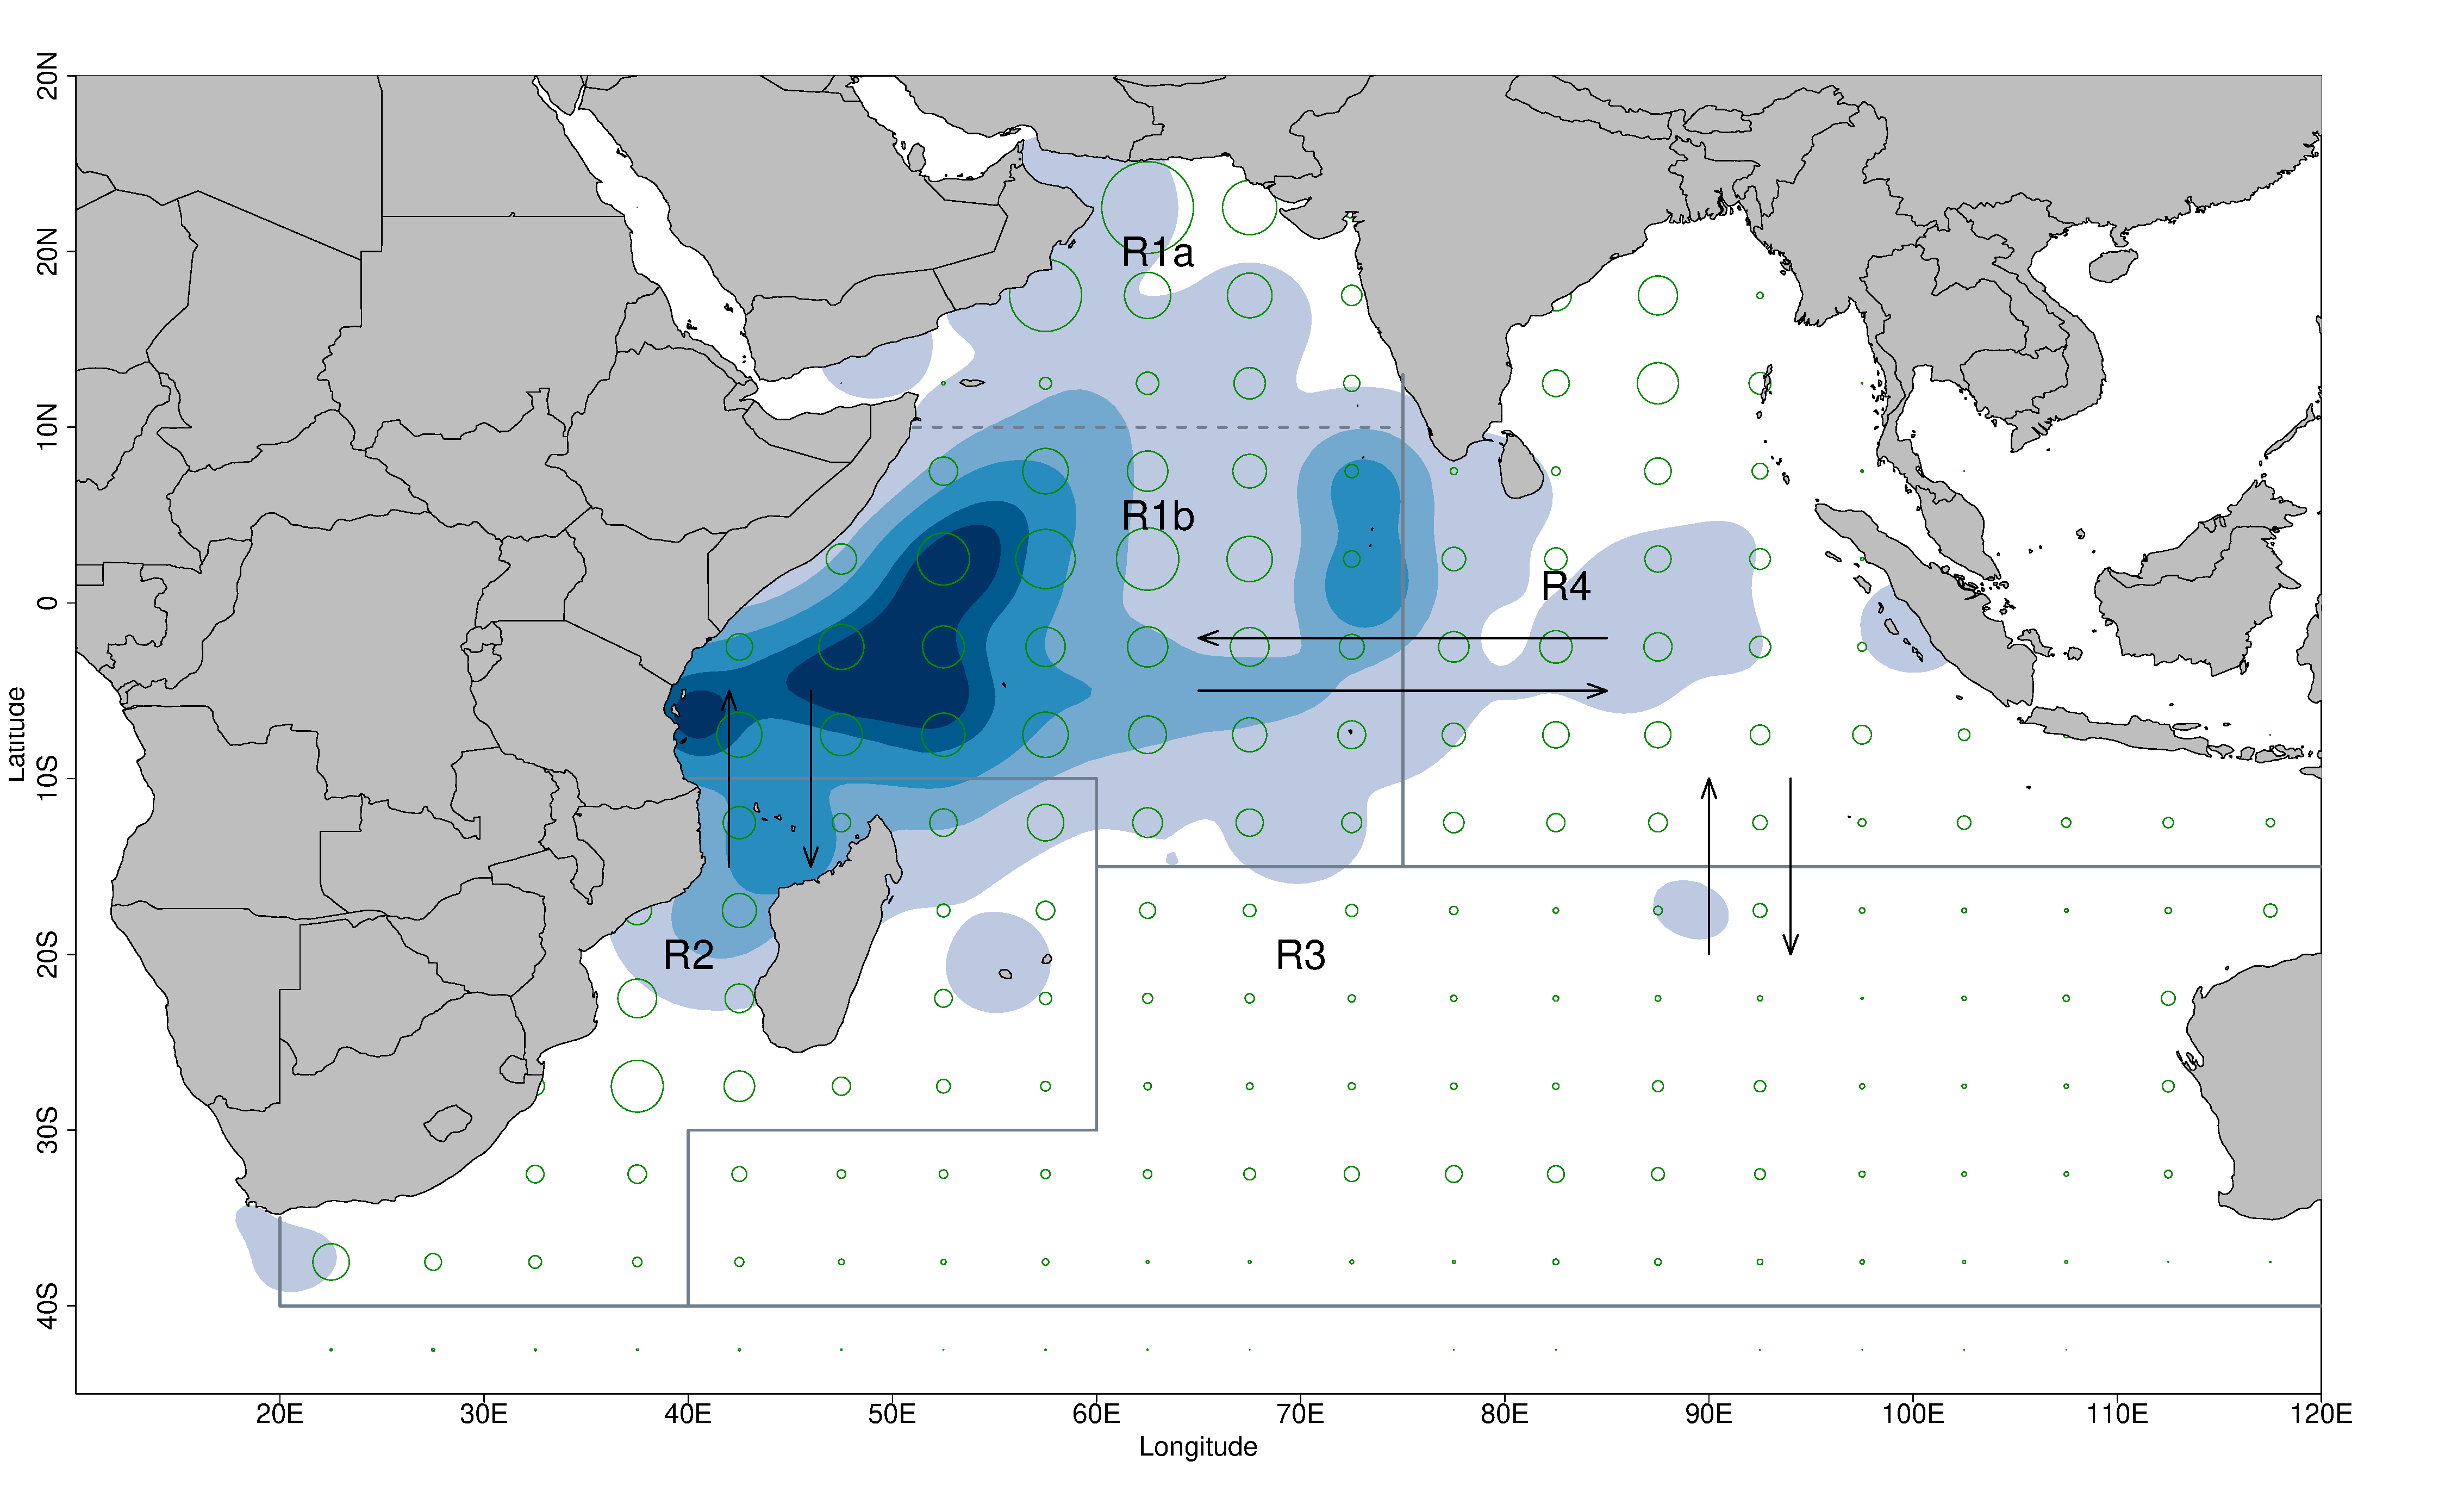
\includegraphics[width=6in]{fig1.eps}
\caption{Spatial stratification of the Indian Ocean for the four region assessment model (R1a and R1b were treated as a single model region R1, but were retained for the fleet definition). The black arrows represent the configuration of the movement parameterization.  Density contours represent of the dispersal of tag releases and subsequent recaptures from Indian Ocean Regional tuna tagging programme. Green circles represent the distribution of catches from the longline fishery aggregated by 5 degree longitude and latitude for 1980 to 2017 (max. = 133 770 t).}
\label{fig:map}
\end{figure*}


\begin{figure}
\centering
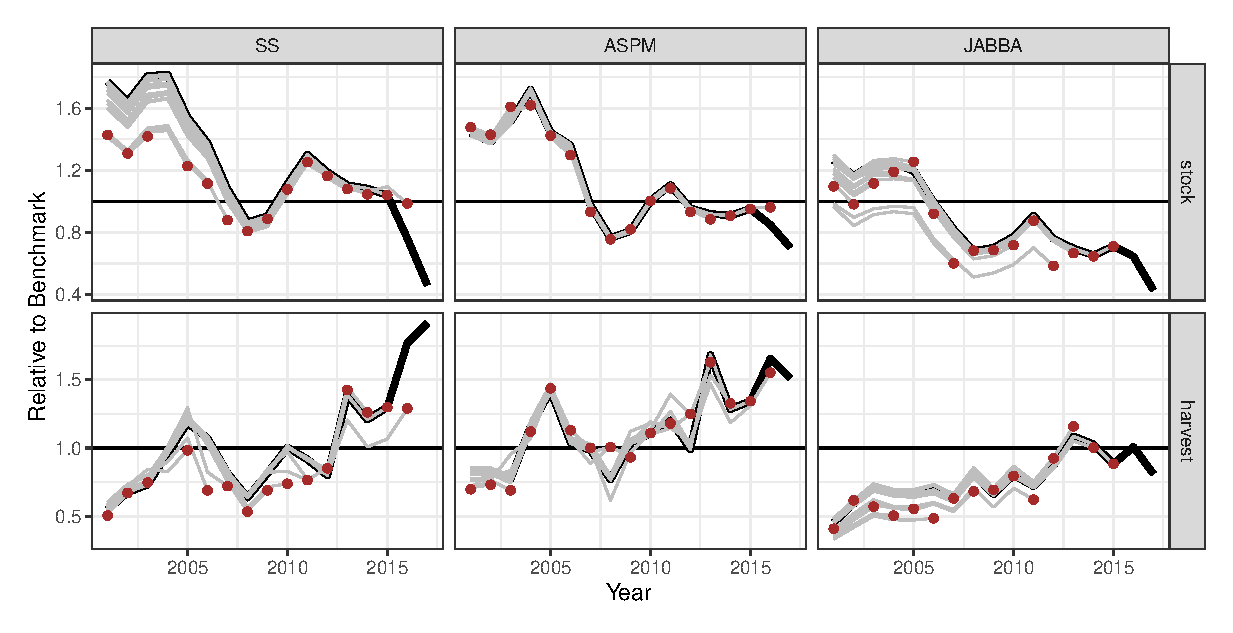
\includegraphics[width=6in]{fig2.eps}
\caption{Hindcasts for one-step ahead, the thick solid line represent the model estimates for $stock$ and $harvest$ relative to $MSY$ benchmarks, based on SSB and instantaneous fishing mortality for SS and ASPM-R and total biomass and harvest rate for JABBA. The points indicate the terminal years of the assessments peeled for the CPUE.}
\label{fig:retro}
\end{figure}


\begin{figure}
\centering
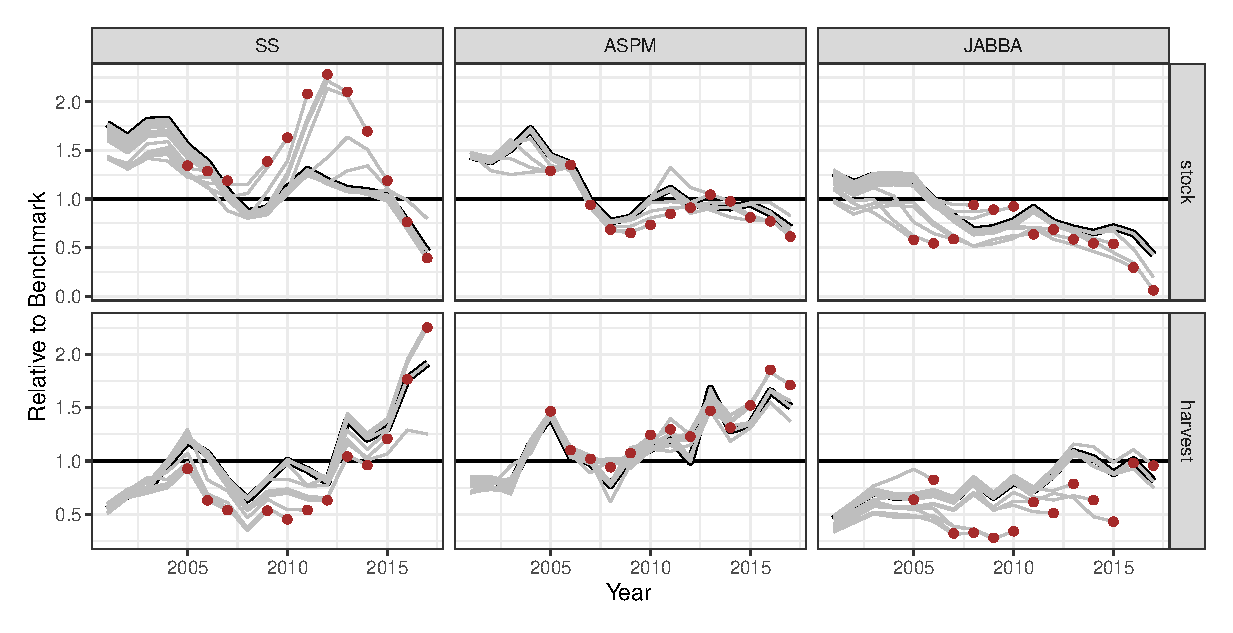
\includegraphics[width=6in]{fig3.eps}
\caption{Hindcasts for three-step ahead, the thick solid line represent the model estimates for $stock$ and $harvest$ relative to $MSY$ benchmarks, based on SSB and instantaneous fishing mortality for SS and ASPM-R and total biomass and harvest rate for JABBA. The points indicate the terminal years of the assessments peeled for the CPUE.}
\label{fig:retro3}
\end{figure}


\begin{figure*}[htbp]
\centering
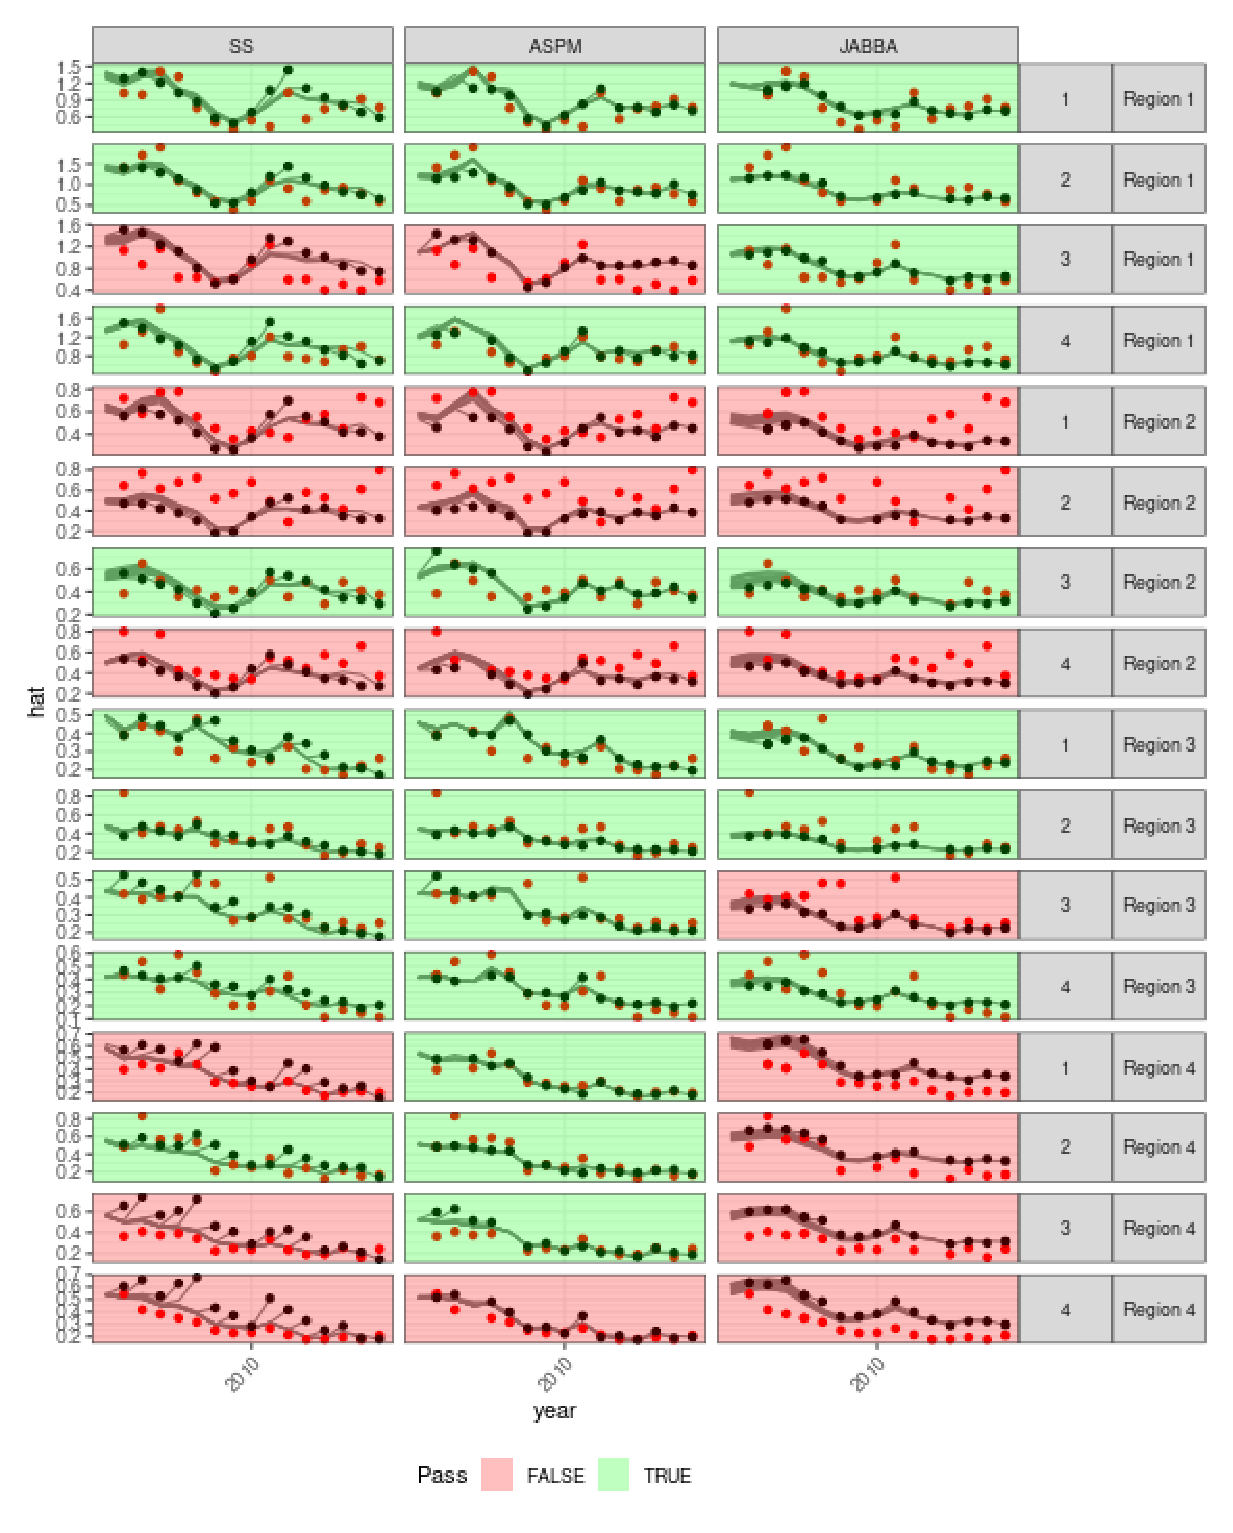
\includegraphics[width=6in]{fig4.eps}
\caption{Hindcasts with one-step ahead for CPUE indices by region and quarter. Green backgrounds indicate that the CPUE index passes Mean Absolute Scaled Error (MASE < 1) criterion, or failed (red) otherwise. Red dots are the observed CPUE values and thin lines are the fits with terminal hincast year indicated by a solid point.}
\label{fig:hy}
\end{figure*}

\begin{figure*}[htbp]
\centering
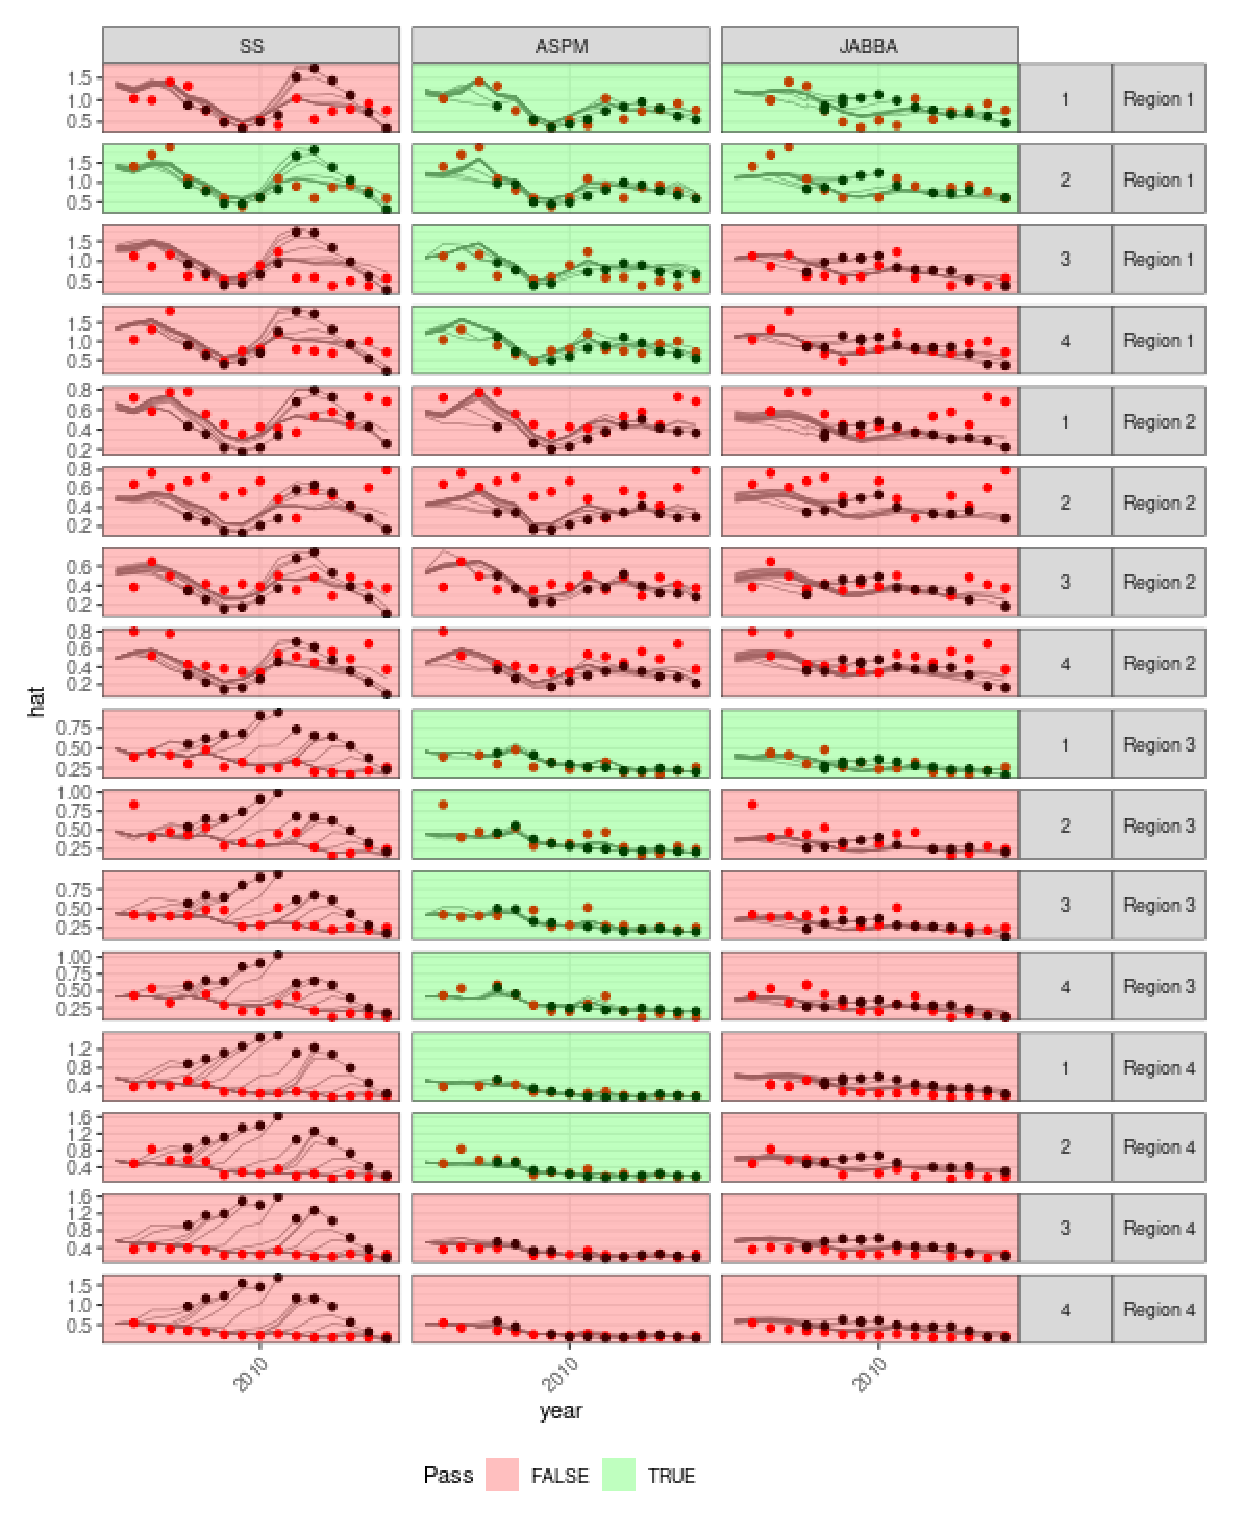
\includegraphics[width=6in]{fig5.eps}
\caption{Hindcasts for three-step ahead for CPUE indices by region and quarter. Green backgrounds indicate that the CPUE index passes Mean Absolute Scaled Error (MASE < 1) criterion, or failed (red) otherwise. Red dots are the observed CPUE values and thin lines are the fits with terminal hincast year indicated by a solid point.}
\label{fig:hy3}
\end{figure*}

\begin{figure*}[htbp]
\centering
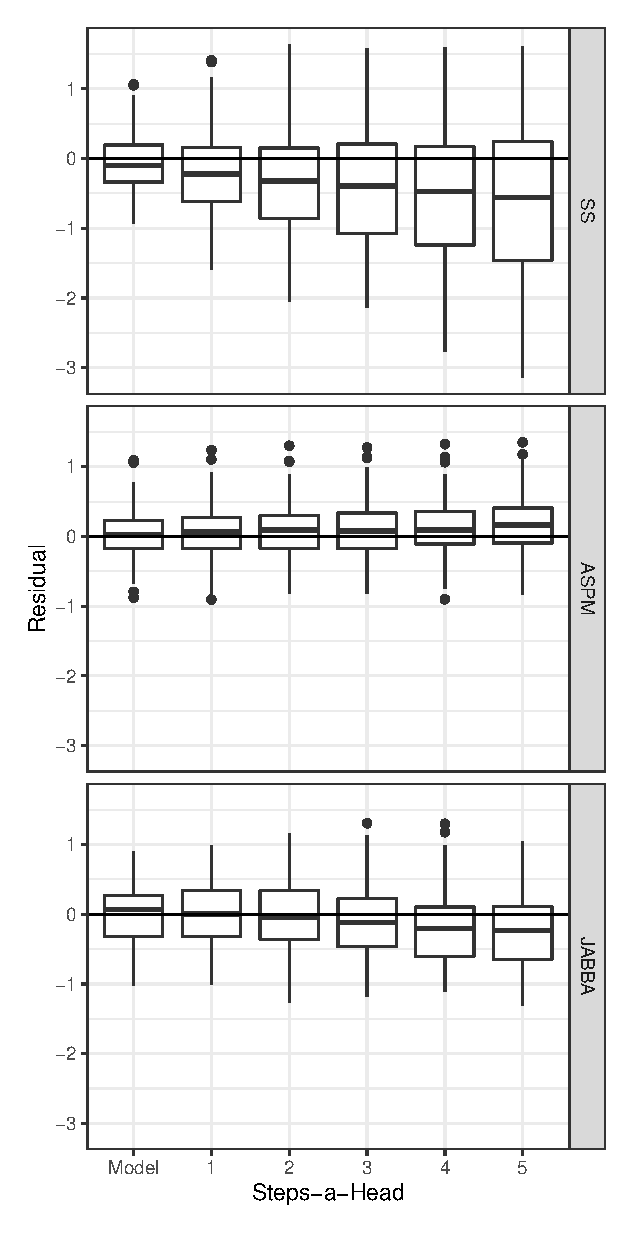
\includegraphics[width=4in]{fig6.eps}
\caption{Boxplots showing model residuals and prediction residuals for 1,2,3,4 and 5 year ahead projections, pooled for all CPUE indices across regions and quarters.}
\label{fig:residuals}
\end{figure*}

\end{document}


\clearpage
\newpage
\section{Tables}


\begin{table}[!ht]
\caption{Summary of Mohn's rho ($\rho_{M}$) statistics for relative stock status estimates from retrospective analysis ($\rho_{M_r}$) and hindcasts with 1 and 3-step ahead projections ($\rho_{M_p}$) using the full Stock Synthesis (SS) reference case, the corresponding Age-Structure Equilibrium Model (ASPM-R) and Bayesian state-space biomass dynamics model JABBA}  
\begin{center}
\label{tab:retro-rho}
\begin{tabular}{|cccc|}
\hline
{\small Quantity} & \small Method & {\small 1-step ahead ($\rho_{M}$)} & {\small 3-step ahead ($\rho_{M_p}$)} \\ 
\hline\hline
{\small $SSB/SSB_{MSY}$     } & {\small SS} 	 & {\small    0.03} & {\small  0.32}      \\
{\small $SSB/SSB_{MSY}$     } & {\small ASPM-R} 	 & {\small    0.06} & {\small -0.09}      \\
{\small $B/B_{MSY}$         } & {\small JABBA} 	 & {\small   -0.03} & {\small -0.21}      \\
{\small $F/F_{MSY}$         } & {\small SS} 	 & {\small   -0.16} & {\small -0.24}      \\
{\small $F/F_{MSY}$         } & {\small ASPM-R} 	 & {\small    0.01} & {\small  0.08}      \\
{\small $U/U_{MSY}$         } & {\small JABBA} 	 & {\small   -0.12} & {\small -0.09}      \\
\hline
\end{tabular}
\end{center}
\end{table}

\begin{table}[ht]
\caption{Mean Absolute Scaled Error (MASE) used for model-free validation of  the full Stock Synthesis (SS) reference case, the corresponding Age-Structure Equilibrium Model (ASPM-R) and Bayesian state-space biomass dynamics model JABBA based on individual CPUE observations by region and quarter. The MASE values are shown for hindcasts with made with 1-year ahead and 3-year ahead projections  }
\begin{center}
\label{tab:mase}
\small
\begin{tabular}{|cc|ccc|ccc|}
\hline
Region & Quarter &    & 1 year & & & 3 year &   \\
     &         & SS & ASPM-R & JABBA & SS & ASPM-R & JABBA  \\
\hline\hline
  1 & 1 & 0.94 & 0.53 & 0.77 & 1.04 & 0.56 & 0.98 \\ 
  1 & 2 & 0.63 & 0.67 & 0.96 & 0.80 & 0.44 & 0.95 \\ 
  1 & 3 & 1.23 & 1.17 & 0.85 & 1.33 & 0.99 & 1.08 \\ 
   1 & 4 & 0.82 & 0.45 & 0.74 & 1.13 & 0.58 & 1.23 \\ 
  2 & 1 & 1.52 & 1.73 & 2.41 & 1.91 & 1.48 & 1.51 \\ 
  2 & 2 & 2.11 & 2.10 & 1.56 & 2.29 & 1.83 & 2.03 \\ 
  2 & 3 & 0.95 & 0.82 & 0.83 & 1.50 & 1.10 & 1.05 \\ 
  2 & 4 & 1.33 & 1.65 & 1.26 & 1.60 & 1.97 & 1.63 \\ 
  3 & 1 & 0.86 & 0.57 & 0.88 & 1.65 & 0.71 & 0.68 \\ 
  3 & 2 & 0.92 & 0.81 & 0.92 & 1.43 & 0.96 & 1.36 \\ 
  3 & 3 & 0.93 & 0.76 & 1.22 & 1.53 & 0.86 & 1.34 \\ 
  3 & 4 & 0.85 & 0.91 & 0.99 & 1.03 & 0.75 & 1.07 \\ 
  4 & 1 & 2.10 & 0.76 & 3.00 & 4.02 & 0.96 & 2.99 \\ 
  4 & 2 & 0.91 & 0.63 & 1.14 & 1.74 & 0.66 & 1.28 \\ 
  4 & 3 & 2.07 & 0.93 & 1.92 & 3.45 & 1.04 & 2.13 \\ 
  4 & 4 & 3.29 & 1.09 & 3.90 & 5.79 & 1.28 & 5.12 \\ 
\hline
\end{tabular}
\end{center}
\end{table}


\clearpage
\newpage
\section{Figures}


\begin{figure*}[!ht]
\centering
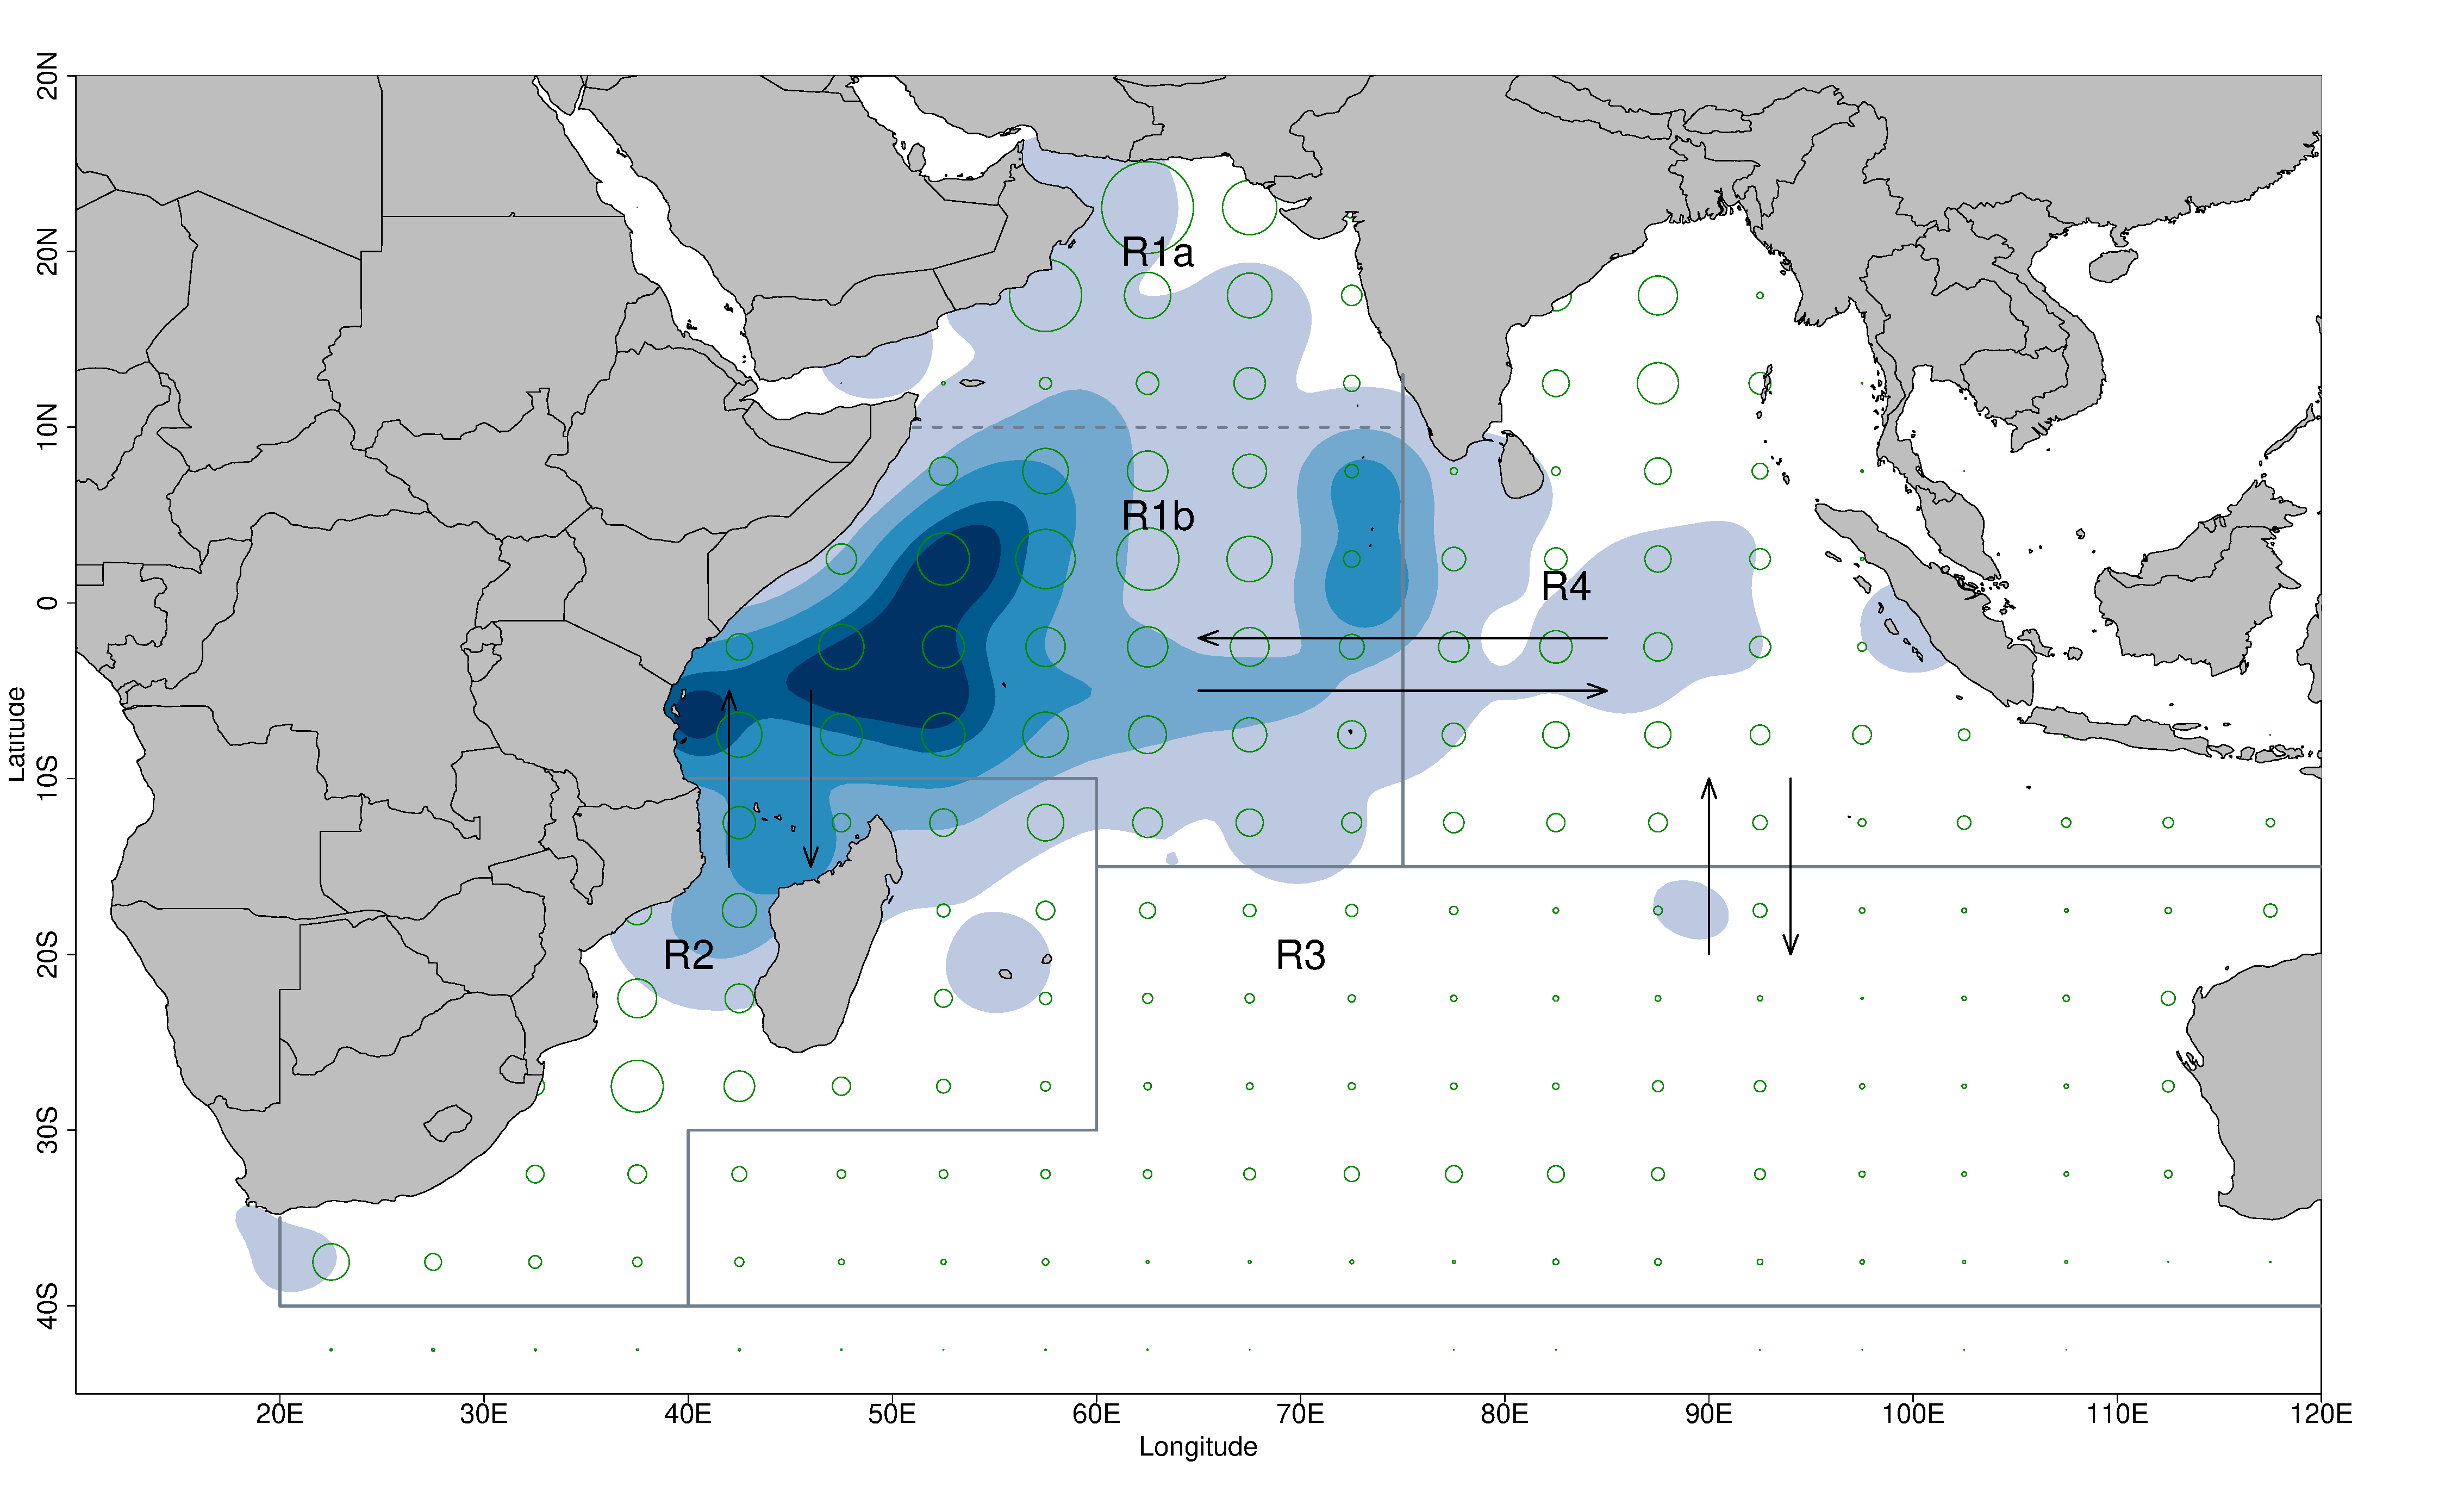
\includegraphics[width=6in]{fig1.eps}
\caption{Spatial stratification of the Indian Ocean for the four region assessment model (R1a and R1b were treated as a single model region R1, but were retained for the fleet definition). The black arrows represent the configuration of the movement parameterization.  Density contours represent of the dispersal of tag releases and subsequent recaptures from Indian Ocean Regional tuna tagging programme. Green circles represent the distribution of catches from the longline fishery aggregated by 5 degree longitude and latitude for 1980 to 2017 (max. = 133 770 t).}
\label{fig:map}
\end{figure*}


\begin{figure}
\centering
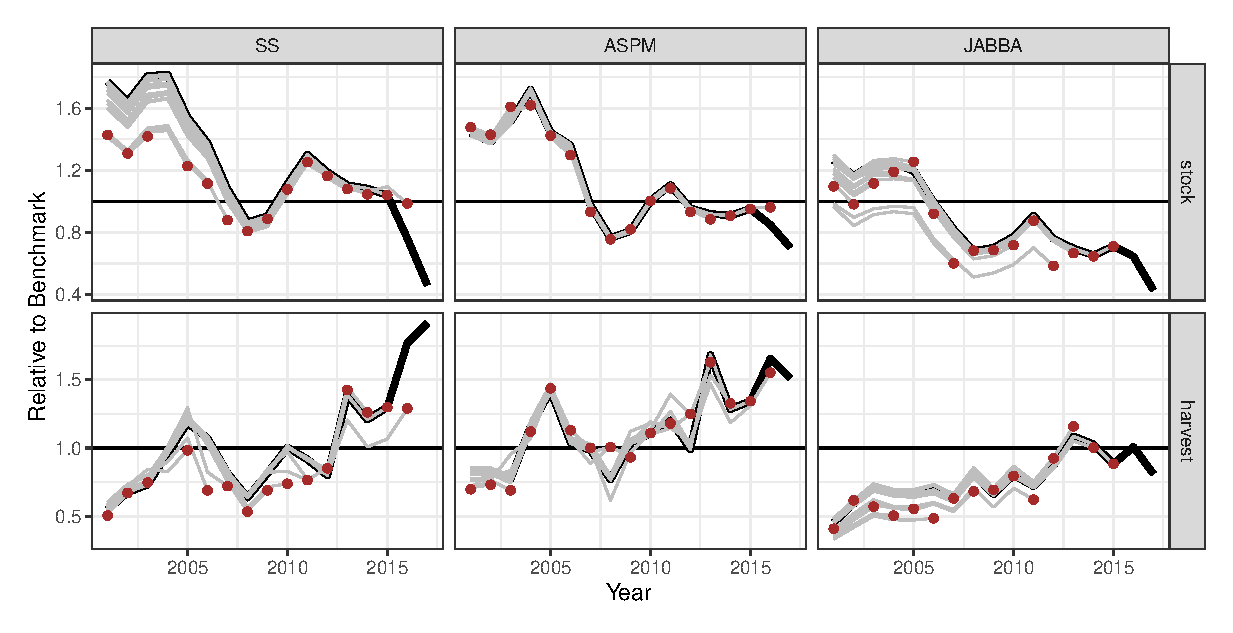
\includegraphics[width=6in]{fig2.eps}
\caption{Hindcasts for one-step ahead, the thick solid line represent the model estimates for $stock$ and $harvest$ relative to $MSY$ benchmarks, based on SSB and instantaneous fishing mortality for SS and ASPM-R and total biomass and harvest rate for JABBA. The points indicate the terminal years of the assessments peeled for the CPUE.}
\label{fig:retro}
\end{figure}


\begin{figure}
\centering
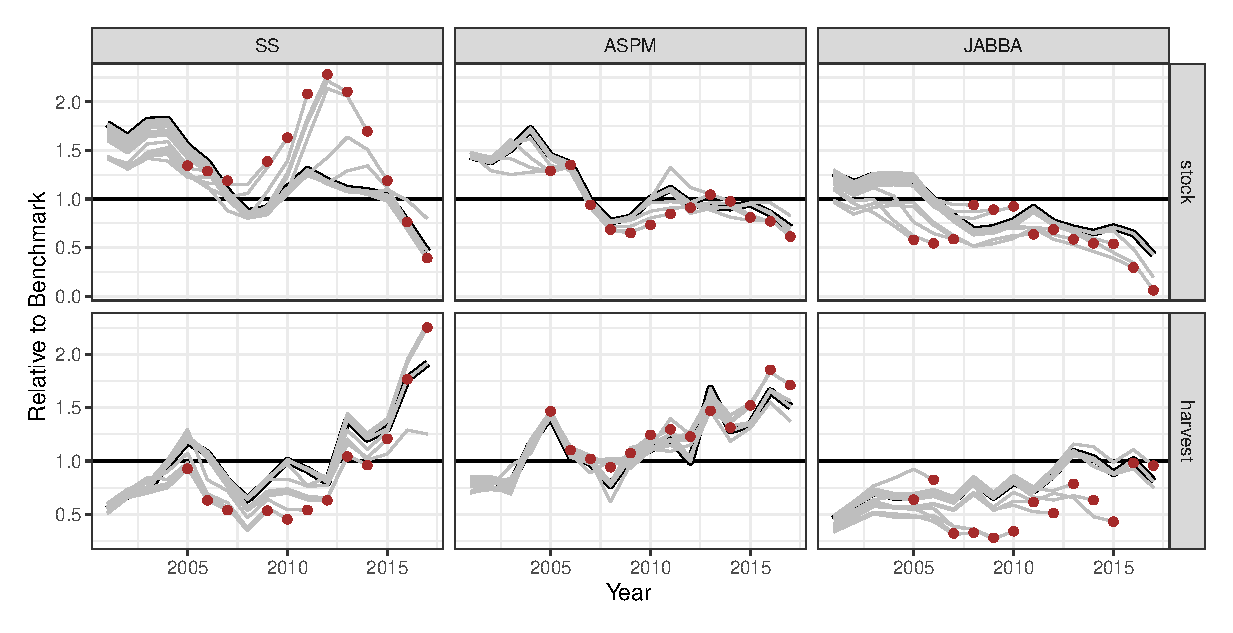
\includegraphics[width=6in]{fig3.eps}
\caption{Hindcasts for three-step ahead, the thick solid line represent the model estimates for $stock$ and $harvest$ relative to $MSY$ benchmarks, based on SSB and instantaneous fishing mortality for SS and ASPM-R and total biomass and harvest rate for JABBA. The points indicate the terminal years of the assessments peeled for the CPUE.}
\label{fig:retro3}
\end{figure}


\begin{figure*}[htbp]
\centering
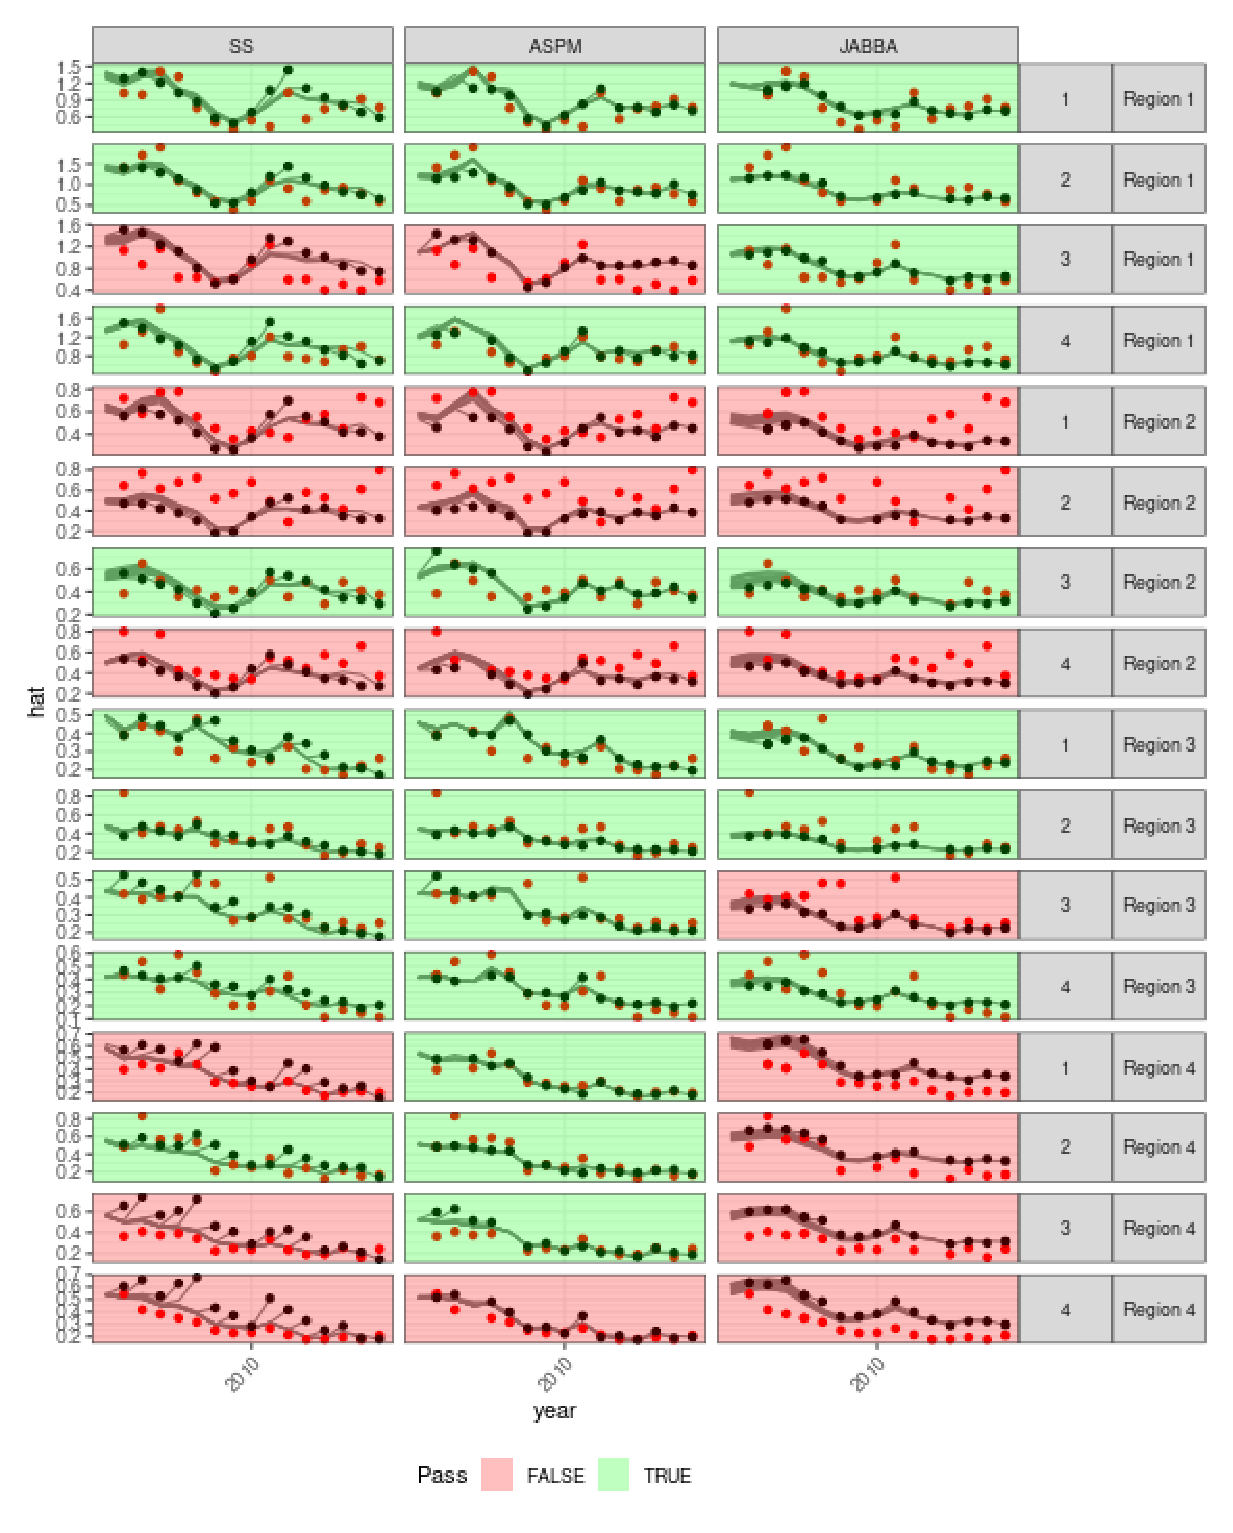
\includegraphics[width=6in]{fig4.eps}
\caption{Hindcasts with one-step ahead for CPUE indices by region and quarter. Green backgrounds indicate that the CPUE index passes Mean Absolute Scaled Error (MASE < 1) criterion, or failed (red) otherwise. Red dots are the observed CPUE values and thin lines are the fits with terminal hincast year indicated by a solid point.}
\label{fig:hy}
\end{figure*}

\begin{figure*}[htbp]
\centering
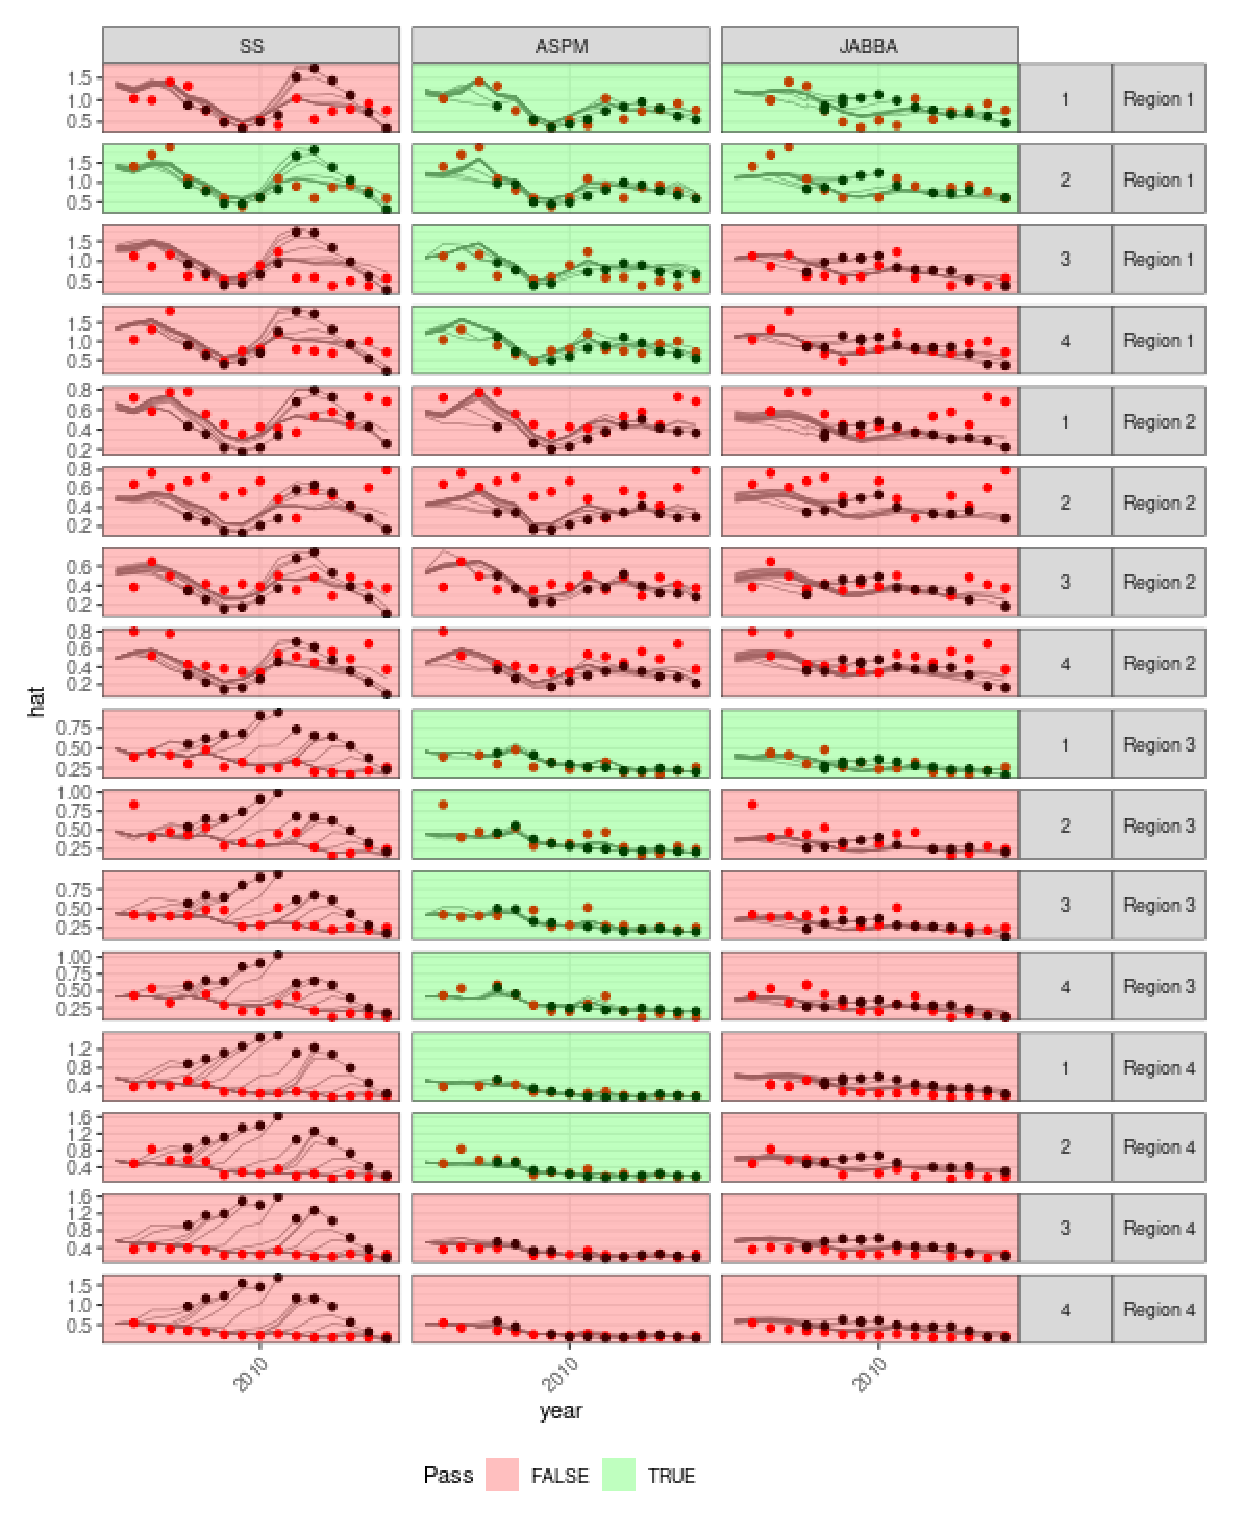
\includegraphics[width=6in]{fig5.eps}
\caption{Hindcasts for three-step ahead for CPUE indices by region and quarter. Green backgrounds indicate that the CPUE index passes Mean Absolute Scaled Error (MASE < 1) criterion, or failed (red) otherwise. Red dots are the observed CPUE values and thin lines are the fits with terminal hincast year indicated by a solid point.}
\label{fig:hy3}
\end{figure*}

\begin{figure*}[htbp]
\centering
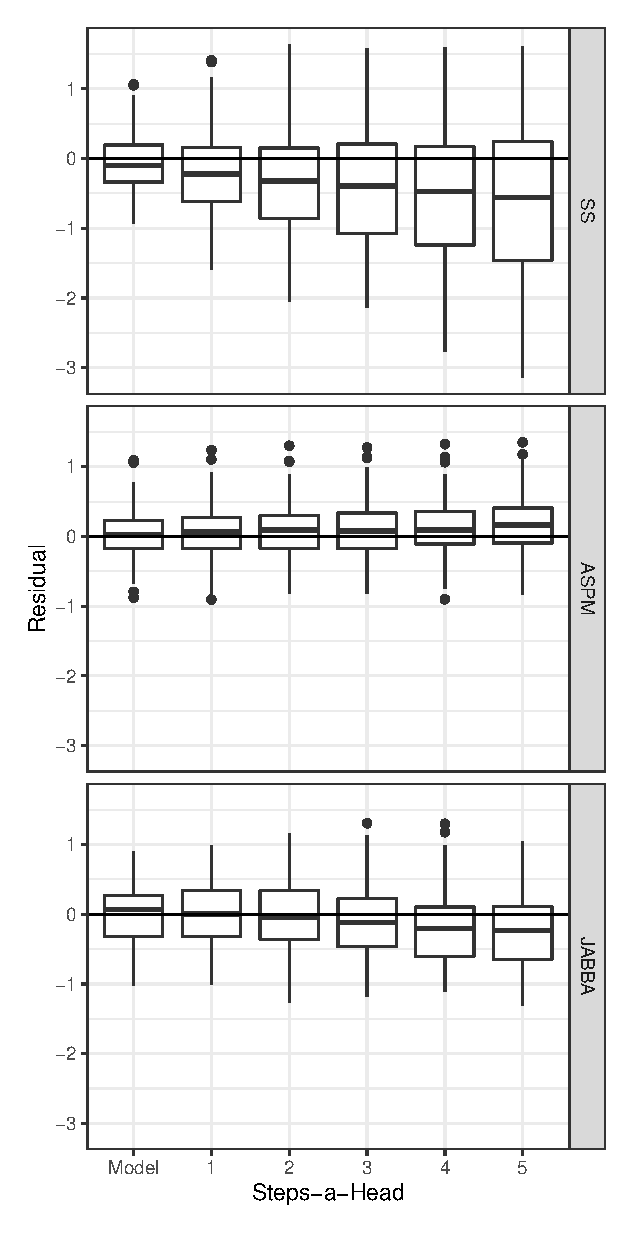
\includegraphics[width=4in]{fig6.eps}
\caption{Boxplots showing model residuals and prediction residuals for 1,2,3,4 and 5 year ahead projections, pooled for all CPUE indices across regions and quarters.}
\label{fig:residuals}
\end{figure*}

\end{document}


\clearpage
\newpage
\section{Tables}


\begin{table}[!ht]
\caption{Summary of Mohn's rho ($\rho_{M}$) statistics for relative stock status estimates from retrospective analysis ($\rho_{M_r}$) and hindcasts with 1 and 3-step ahead projections ($\rho_{M_p}$) using the full Stock Synthesis (SS) reference case, the corresponding Age-Structure Equilibrium Model (ASPM-R) and Bayesian state-space biomass dynamics model JABBA}  
\begin{center}
\label{tab:retro-rho}
\begin{tabular}{|cccc|}
\hline
{\small Quantity} & \small Method & {\small 1-step ahead ($\rho_{M}$)} & {\small 3-step ahead ($\rho_{M_p}$)} \\ 
\hline\hline
{\small $SSB/SSB_{MSY}$     } & {\small SS} 	 & {\small    0.03} & {\small  0.32}      \\
{\small $SSB/SSB_{MSY}$     } & {\small ASPM-R} 	 & {\small    0.06} & {\small -0.09}      \\
{\small $B/B_{MSY}$         } & {\small JABBA} 	 & {\small   -0.03} & {\small -0.21}      \\
{\small $F/F_{MSY}$         } & {\small SS} 	 & {\small   -0.16} & {\small -0.24}      \\
{\small $F/F_{MSY}$         } & {\small ASPM-R} 	 & {\small    0.01} & {\small  0.08}      \\
{\small $U/U_{MSY}$         } & {\small JABBA} 	 & {\small   -0.12} & {\small -0.09}      \\
\hline
\end{tabular}
\end{center}
\end{table}

\begin{table}[ht]
\caption{Mean Absolute Scaled Error (MASE) used for model-free validation of  the full Stock Synthesis (SS) reference case, the corresponding Age-Structure Equilibrium Model (ASPM-R) and Bayesian state-space biomass dynamics model JABBA based on individual CPUE observations by region and quarter. The MASE values are shown for hindcasts with made with 1-year ahead and 3-year ahead projections  }
\begin{center}
\label{tab:mase}
\small
\begin{tabular}{|cc|ccc|ccc|}
\hline
Region & Quarter &    & 1 year & & & 3 year &   \\
     &         & SS & ASPM-R & JABBA & SS & ASPM-R & JABBA  \\
\hline\hline
  1 & 1 & 0.94 & 0.53 & 0.77 & 1.04 & 0.56 & 0.98 \\ 
  1 & 2 & 0.63 & 0.67 & 0.96 & 0.80 & 0.44 & 0.95 \\ 
  1 & 3 & 1.23 & 1.17 & 0.85 & 1.33 & 0.99 & 1.08 \\ 
   1 & 4 & 0.82 & 0.45 & 0.74 & 1.13 & 0.58 & 1.23 \\ 
  2 & 1 & 1.52 & 1.73 & 2.41 & 1.91 & 1.48 & 1.51 \\ 
  2 & 2 & 2.11 & 2.10 & 1.56 & 2.29 & 1.83 & 2.03 \\ 
  2 & 3 & 0.95 & 0.82 & 0.83 & 1.50 & 1.10 & 1.05 \\ 
  2 & 4 & 1.33 & 1.65 & 1.26 & 1.60 & 1.97 & 1.63 \\ 
  3 & 1 & 0.86 & 0.57 & 0.88 & 1.65 & 0.71 & 0.68 \\ 
  3 & 2 & 0.92 & 0.81 & 0.92 & 1.43 & 0.96 & 1.36 \\ 
  3 & 3 & 0.93 & 0.76 & 1.22 & 1.53 & 0.86 & 1.34 \\ 
  3 & 4 & 0.85 & 0.91 & 0.99 & 1.03 & 0.75 & 1.07 \\ 
  4 & 1 & 2.10 & 0.76 & 3.00 & 4.02 & 0.96 & 2.99 \\ 
  4 & 2 & 0.91 & 0.63 & 1.14 & 1.74 & 0.66 & 1.28 \\ 
  4 & 3 & 2.07 & 0.93 & 1.92 & 3.45 & 1.04 & 2.13 \\ 
  4 & 4 & 3.29 & 1.09 & 3.90 & 5.79 & 1.28 & 5.12 \\ 
\hline
\end{tabular}
\end{center}
\end{table}


\clearpage
\newpage
\section{Figures}


\begin{figure*}[!ht]
\centering
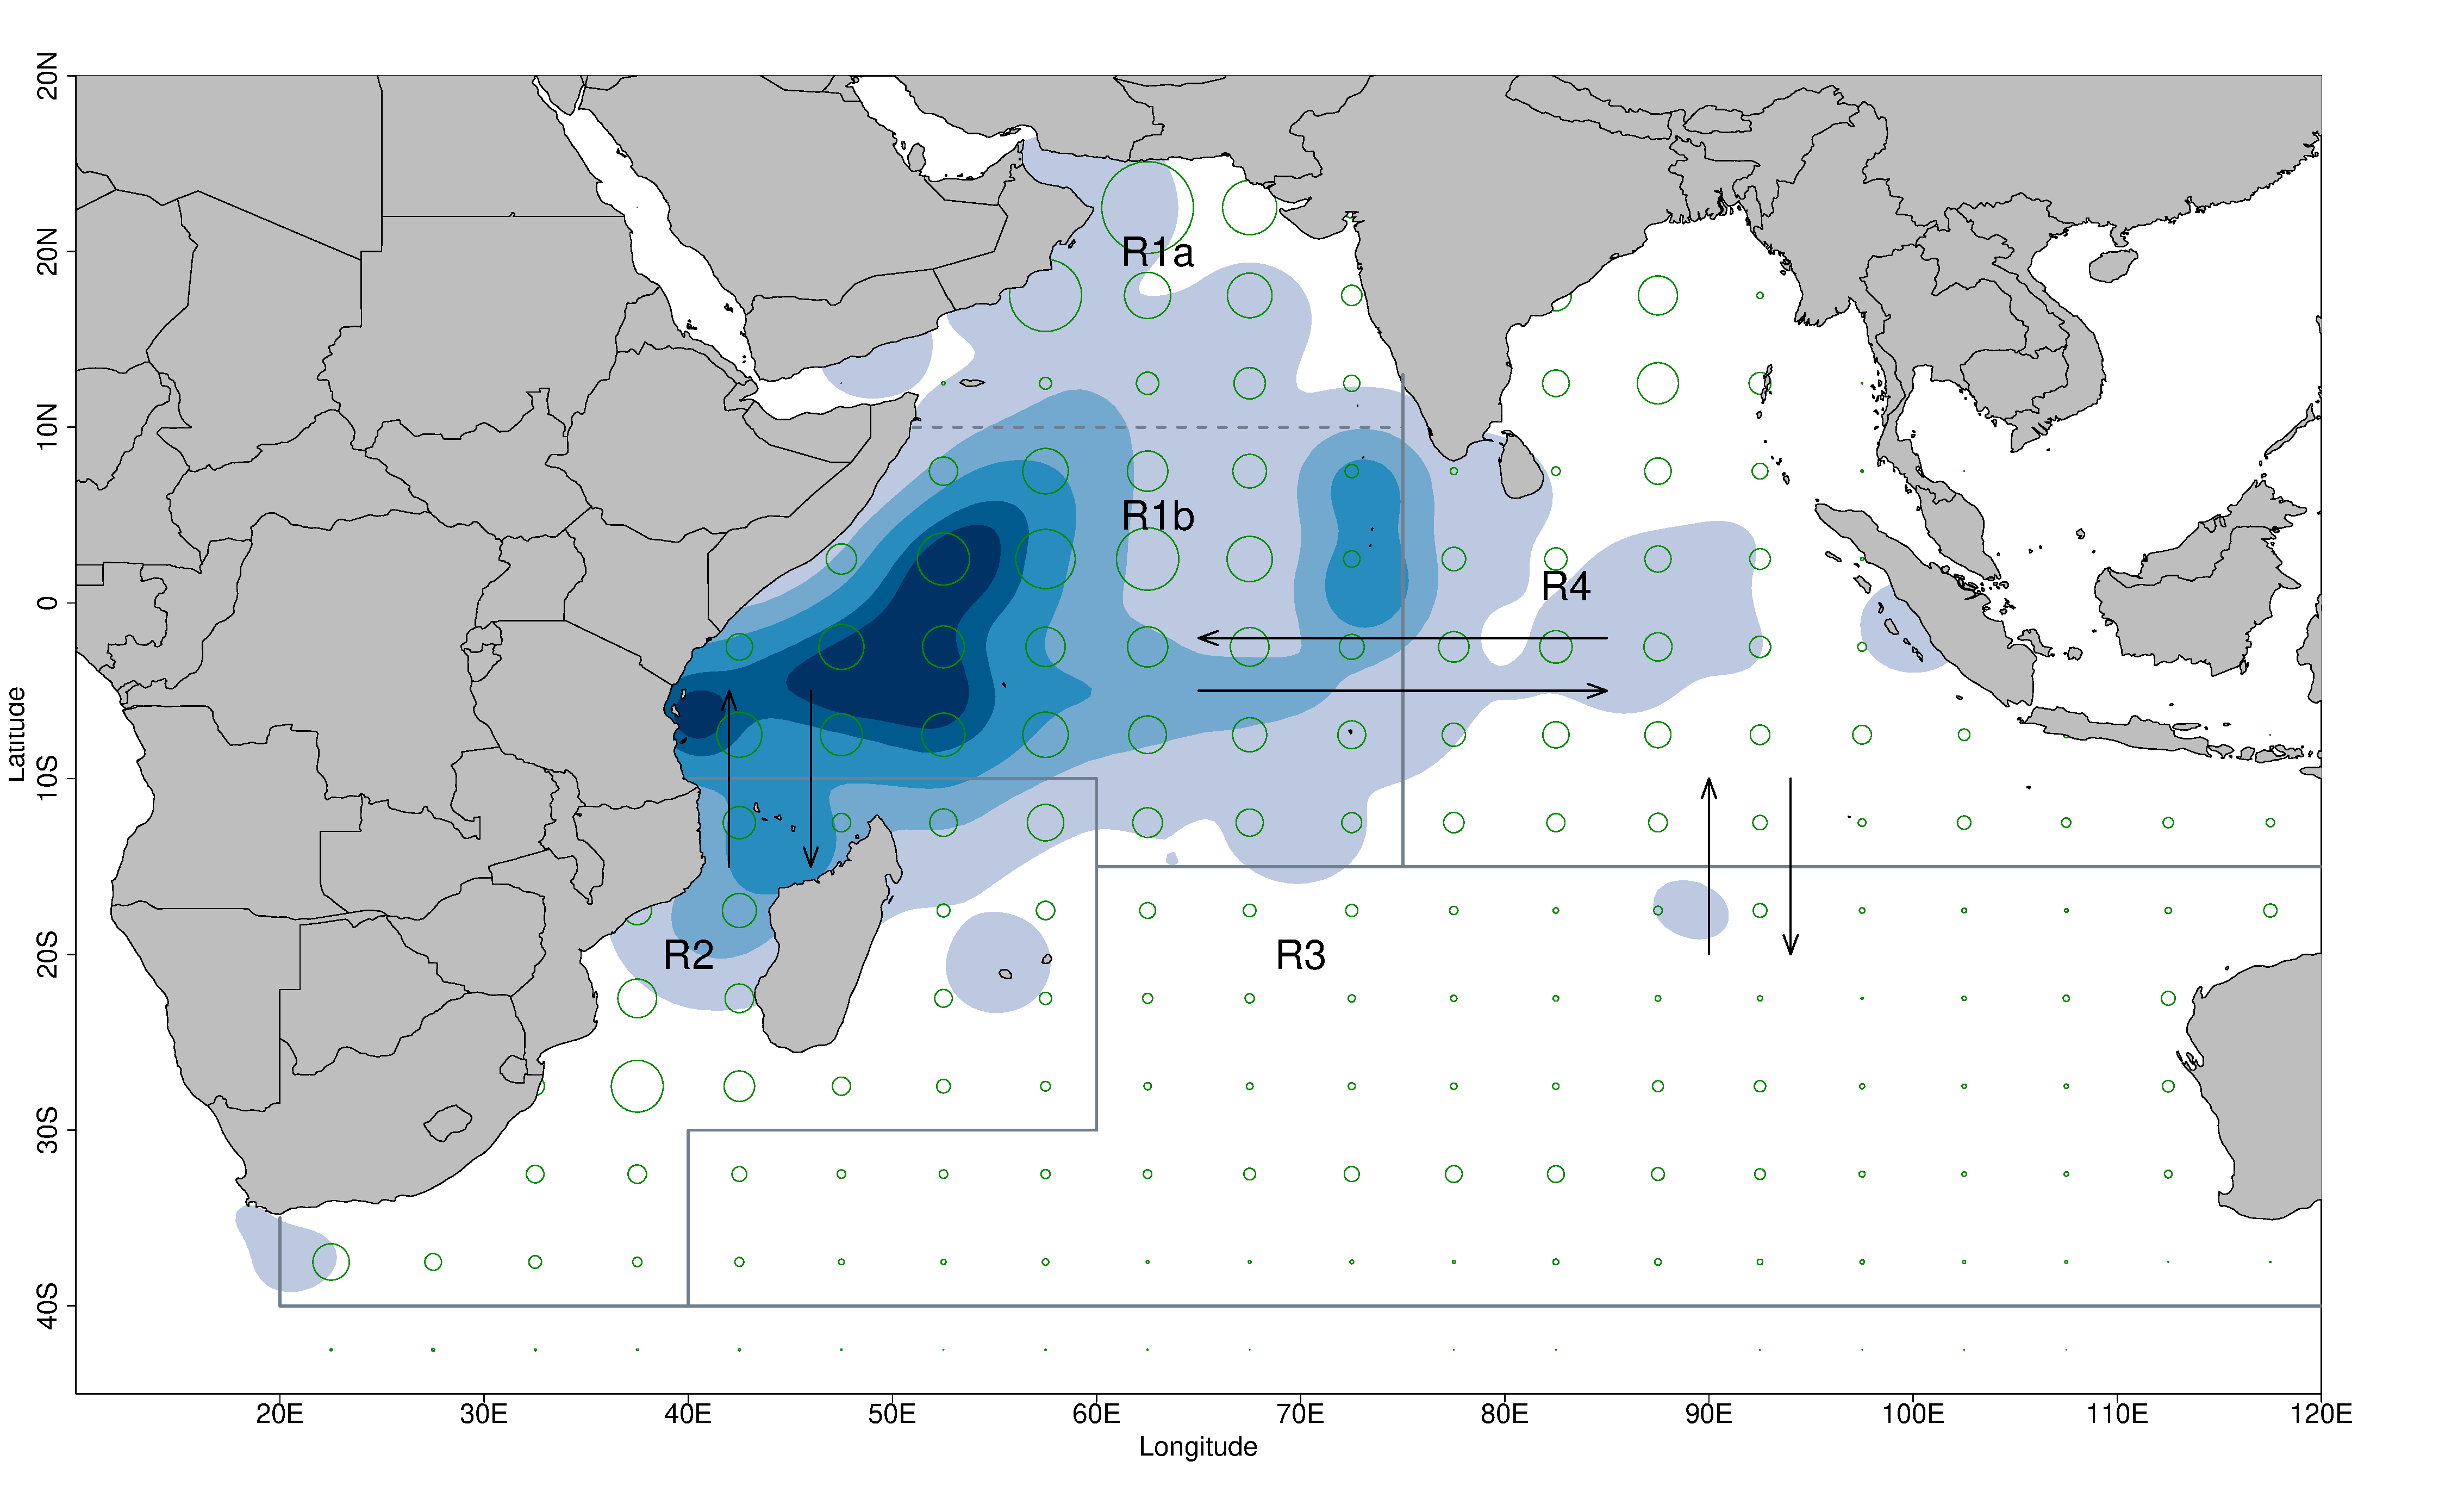
\includegraphics[width=6in]{fig1.eps}
\caption{Spatial stratification of the Indian Ocean for the four region assessment model (R1a and R1b were treated as a single model region R1, but were retained for the fleet definition). The black arrows represent the configuration of the movement parameterization.  Density contours represent of the dispersal of tag releases and subsequent recaptures from Indian Ocean Regional tuna tagging programme. Green circles represent the distribution of catches from the longline fishery aggregated by 5 degree longitude and latitude for 1980 to 2017 (max. = 133 770 t).}
\label{fig:map}
\end{figure*}


\begin{figure}
\centering
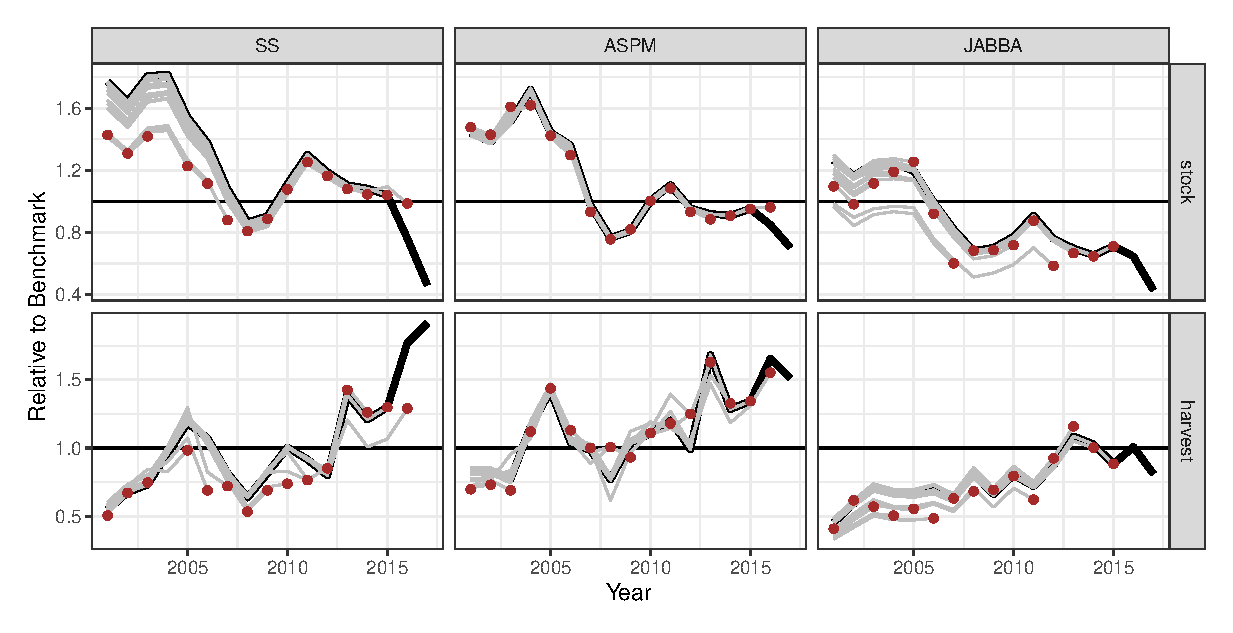
\includegraphics[width=6in]{fig2.eps}
\caption{Hindcasts for one-step ahead, the thick solid line represent the model estimates for $stock$ and $harvest$ relative to $MSY$ benchmarks, based on SSB and instantaneous fishing mortality for SS and ASPM-R and total biomass and harvest rate for JABBA. The points indicate the terminal years of the assessments peeled for the CPUE.}
\label{fig:retro}
\end{figure}


\begin{figure}
\centering
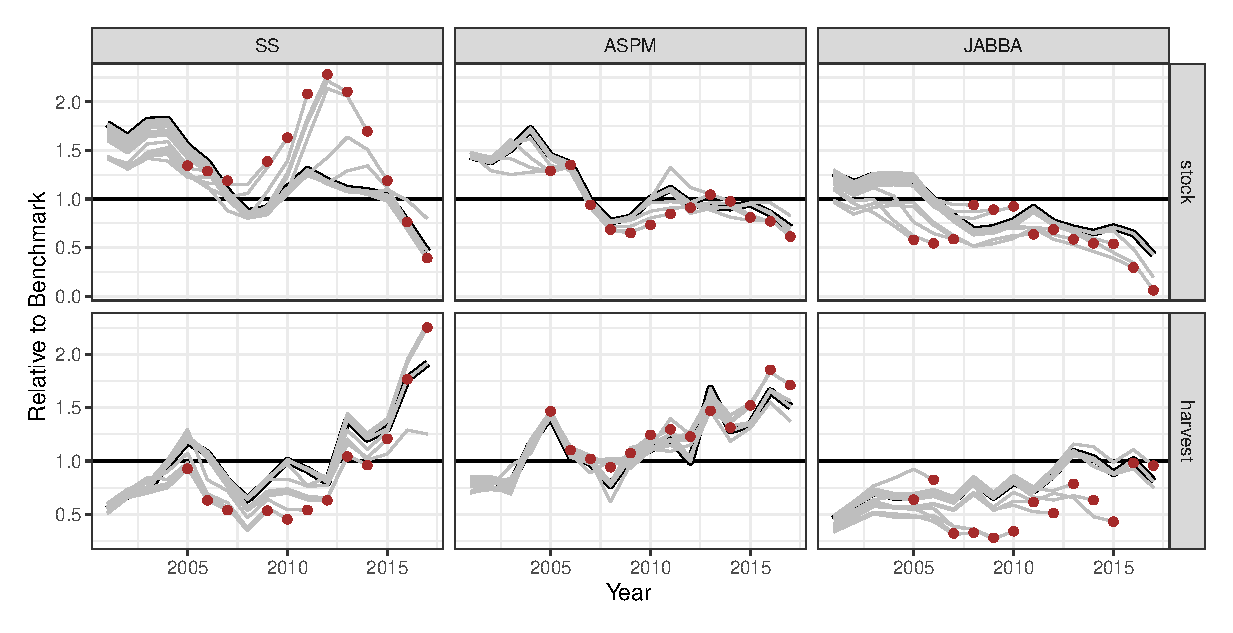
\includegraphics[width=6in]{fig3.eps}
\caption{Hindcasts for three-step ahead, the thick solid line represent the model estimates for $stock$ and $harvest$ relative to $MSY$ benchmarks, based on SSB and instantaneous fishing mortality for SS and ASPM-R and total biomass and harvest rate for JABBA. The points indicate the terminal years of the assessments peeled for the CPUE.}
\label{fig:retro3}
\end{figure}


\begin{figure*}[htbp]
\centering
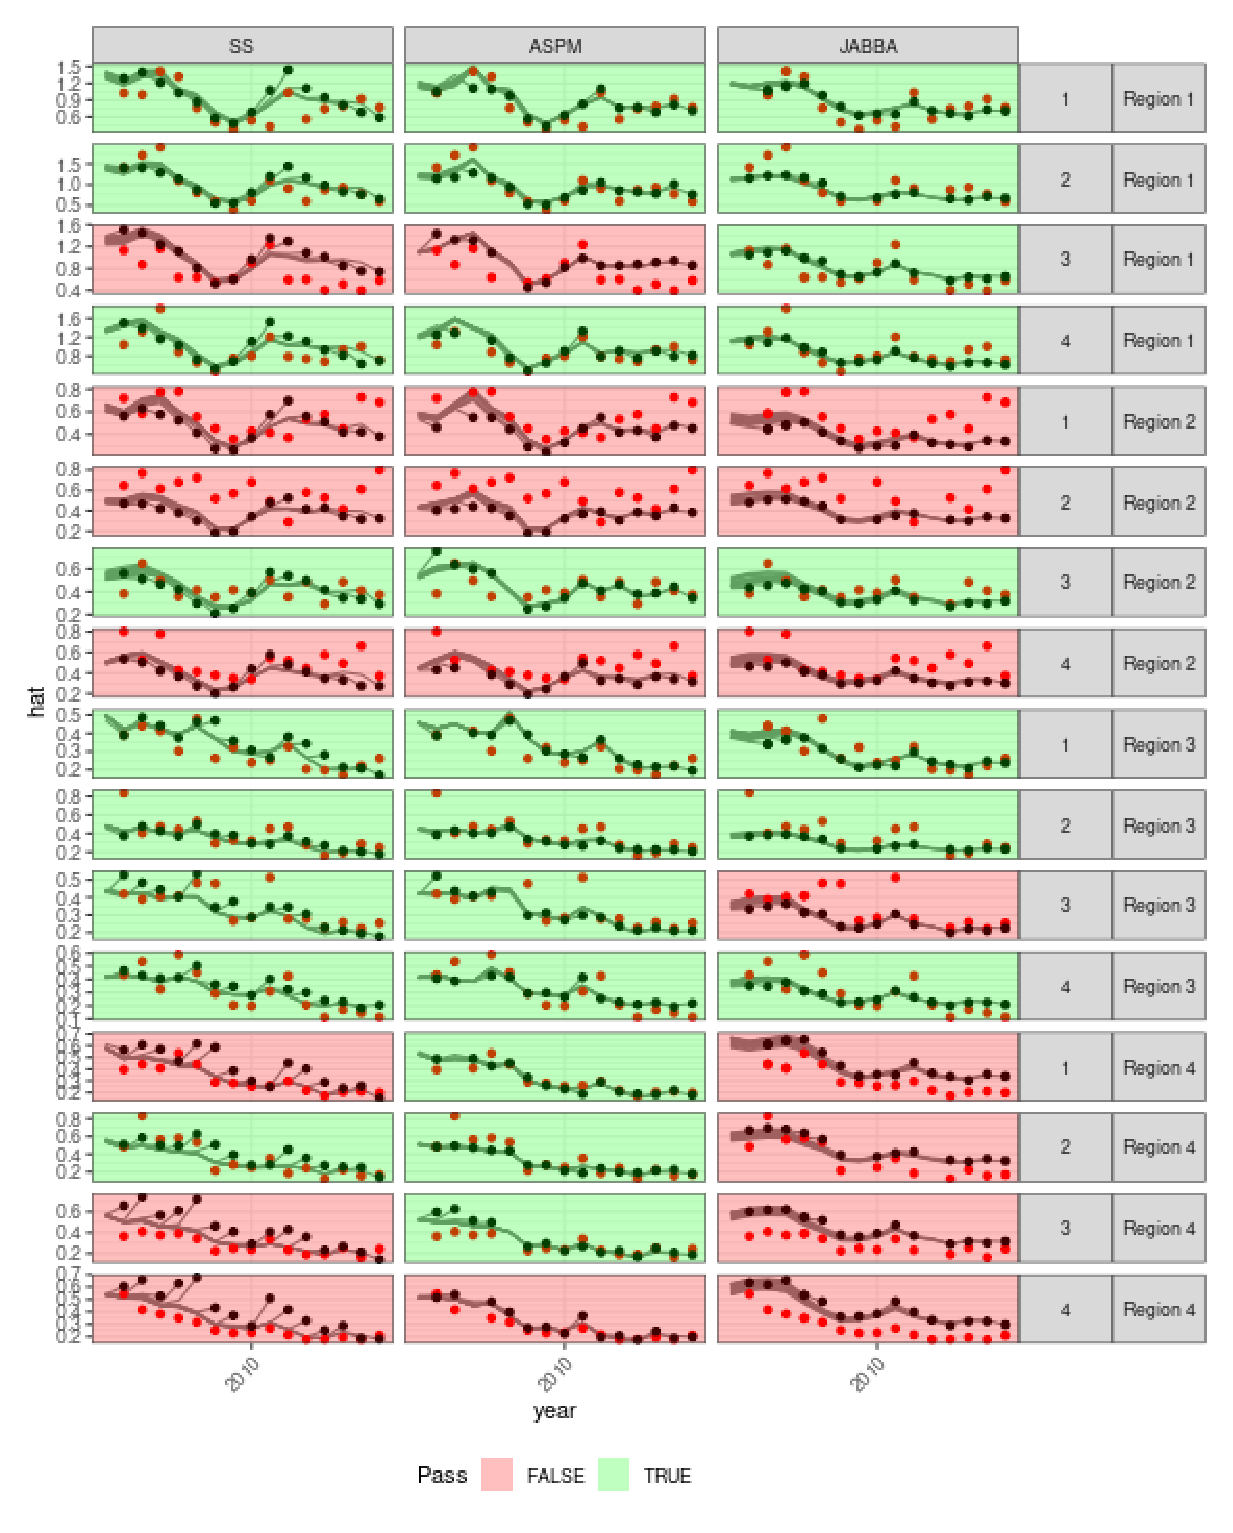
\includegraphics[width=6in]{fig4.eps}
\caption{Hindcasts with one-step ahead for CPUE indices by region and quarter. Green backgrounds indicate that the CPUE index passes Mean Absolute Scaled Error (MASE < 1) criterion, or failed (red) otherwise. Red dots are the observed CPUE values and thin lines are the fits with terminal hincast year indicated by a solid point.}
\label{fig:hy}
\end{figure*}

\begin{figure*}[htbp]
\centering
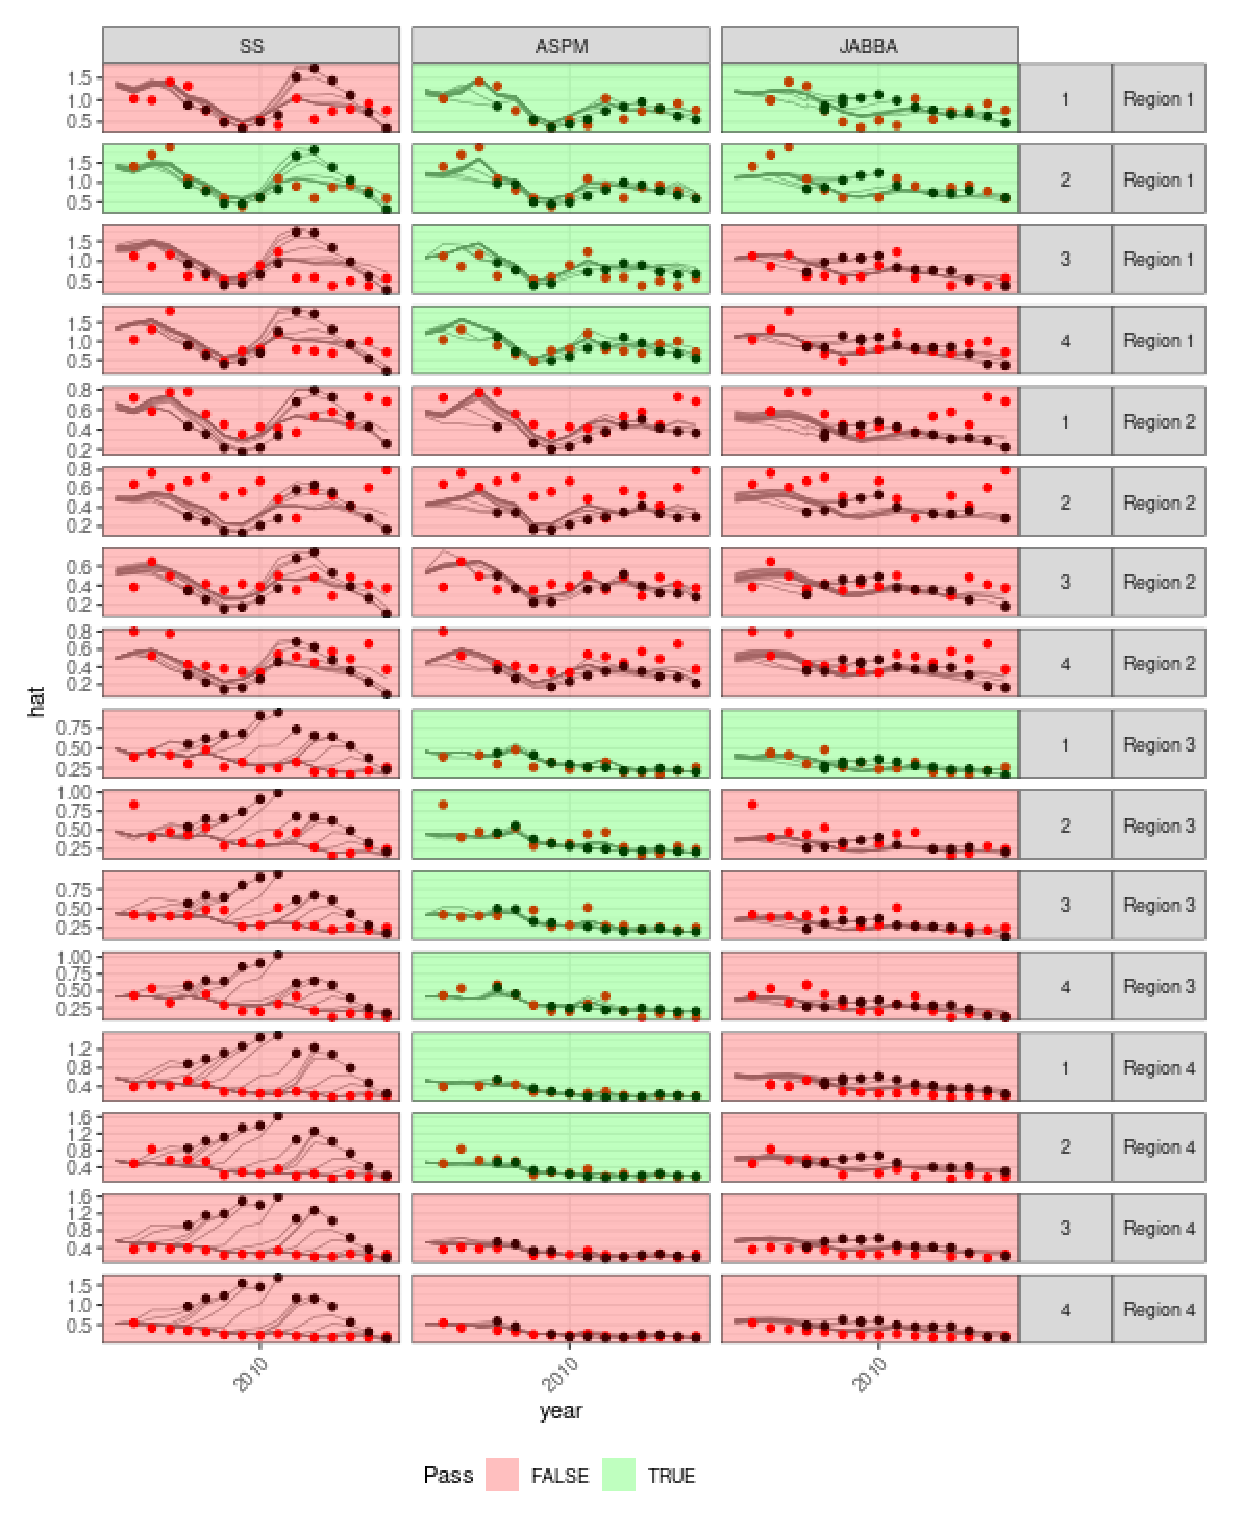
\includegraphics[width=6in]{fig5.eps}
\caption{Hindcasts for three-step ahead for CPUE indices by region and quarter. Green backgrounds indicate that the CPUE index passes Mean Absolute Scaled Error (MASE < 1) criterion, or failed (red) otherwise. Red dots are the observed CPUE values and thin lines are the fits with terminal hincast year indicated by a solid point.}
\label{fig:hy3}
\end{figure*}

\begin{figure*}[htbp]
\centering
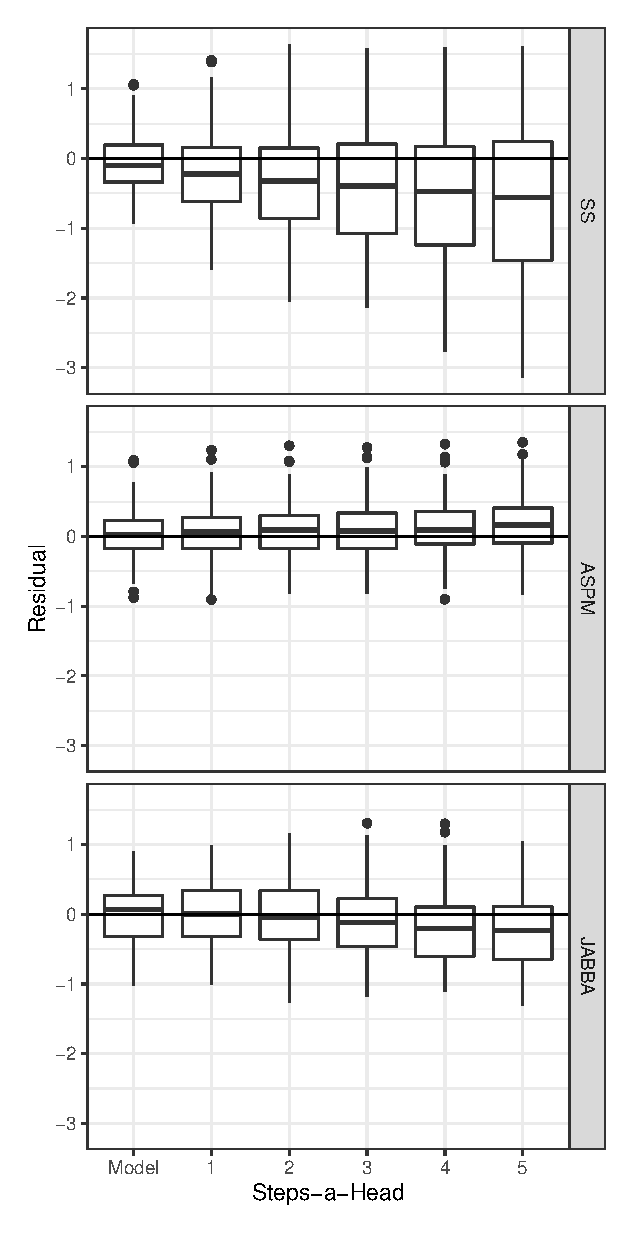
\includegraphics[width=4in]{fig6.eps}
\caption{Boxplots showing model residuals and prediction residuals for 1,2,3,4 and 5 year ahead projections, pooled for all CPUE indices across regions and quarters.}
\label{fig:residuals}
\end{figure*}

\end{document}


\clearpage
\newpage
\section{Tables}


\begin{table}[!ht]
\caption{Summary of Mohn's rho ($\rho_{M}$) statistics for relative stock status estimates from retrospective analysis ($\rho_{M_r}$) and hindcasts with 1 and 3-step ahead projections ($\rho_{M_p}$) using the full Stock Synthesis (SS) reference case, the corresponding Age-Structure Equilibrium Model (ASPM-R) and Bayesian state-space biomass dynamics model JABBA}  
\begin{center}
\label{tab:retro-rho}
\begin{tabular}{|cccc|}
\hline
{\small Quantity} & \small Method & {\small 1-step ahead ($\rho_{M}$)} & {\small 3-step ahead ($\rho_{M_p}$)} \\ 
\hline\hline
{\small $SSB/SSB_{MSY}$     } & {\small SS} 	 & {\small    0.03} & {\small  0.32}      \\
{\small $SSB/SSB_{MSY}$     } & {\small ASPM-R} 	 & {\small    0.06} & {\small -0.09}      \\
{\small $B/B_{MSY}$         } & {\small JABBA} 	 & {\small   -0.03} & {\small -0.21}      \\
{\small $F/F_{MSY}$         } & {\small SS} 	 & {\small   -0.16} & {\small -0.24}      \\
{\small $F/F_{MSY}$         } & {\small ASPM-R} 	 & {\small    0.01} & {\small  0.08}      \\
{\small $U/U_{MSY}$         } & {\small JABBA} 	 & {\small   -0.12} & {\small -0.09}      \\
\hline
\end{tabular}
\end{center}
\end{table}

\begin{table}[ht]
\caption{Mean Absolute Scaled Error (MASE) used for model-free validation of  the full Stock Synthesis (SS) reference case, the corresponding Age-Structure Equilibrium Model (ASPM-R) and Bayesian state-space biomass dynamics model JABBA based on individual CPUE observations by region and quarter. The MASE values are shown for hindcasts with made with 1-year ahead and 3-year ahead projections  }
\begin{center}
\label{tab:mase}
\small
\begin{tabular}{|cc|ccc|ccc|}
\hline
Region & Quarter &    & 1 year & & & 3 year &   \\
     &         & SS & ASPM-R & JABBA & SS & ASPM-R & JABBA  \\
\hline\hline
  1 & 1 & 0.94 & 0.53 & 0.77 & 1.04 & 0.56 & 0.98 \\ 
  1 & 2 & 0.63 & 0.67 & 0.96 & 0.80 & 0.44 & 0.95 \\ 
  1 & 3 & 1.23 & 1.17 & 0.85 & 1.33 & 0.99 & 1.08 \\ 
   1 & 4 & 0.82 & 0.45 & 0.74 & 1.13 & 0.58 & 1.23 \\ 
  2 & 1 & 1.52 & 1.73 & 2.41 & 1.91 & 1.48 & 1.51 \\ 
  2 & 2 & 2.11 & 2.10 & 1.56 & 2.29 & 1.83 & 2.03 \\ 
  2 & 3 & 0.95 & 0.82 & 0.83 & 1.50 & 1.10 & 1.05 \\ 
  2 & 4 & 1.33 & 1.65 & 1.26 & 1.60 & 1.97 & 1.63 \\ 
  3 & 1 & 0.86 & 0.57 & 0.88 & 1.65 & 0.71 & 0.68 \\ 
  3 & 2 & 0.92 & 0.81 & 0.92 & 1.43 & 0.96 & 1.36 \\ 
  3 & 3 & 0.93 & 0.76 & 1.22 & 1.53 & 0.86 & 1.34 \\ 
  3 & 4 & 0.85 & 0.91 & 0.99 & 1.03 & 0.75 & 1.07 \\ 
  4 & 1 & 2.10 & 0.76 & 3.00 & 4.02 & 0.96 & 2.99 \\ 
  4 & 2 & 0.91 & 0.63 & 1.14 & 1.74 & 0.66 & 1.28 \\ 
  4 & 3 & 2.07 & 0.93 & 1.92 & 3.45 & 1.04 & 2.13 \\ 
  4 & 4 & 3.29 & 1.09 & 3.90 & 5.79 & 1.28 & 5.12 \\ 
\hline
\end{tabular}
\end{center}
\end{table}


\clearpage
\newpage
\section{Figures}


\begin{figure*}[!ht]
\centering
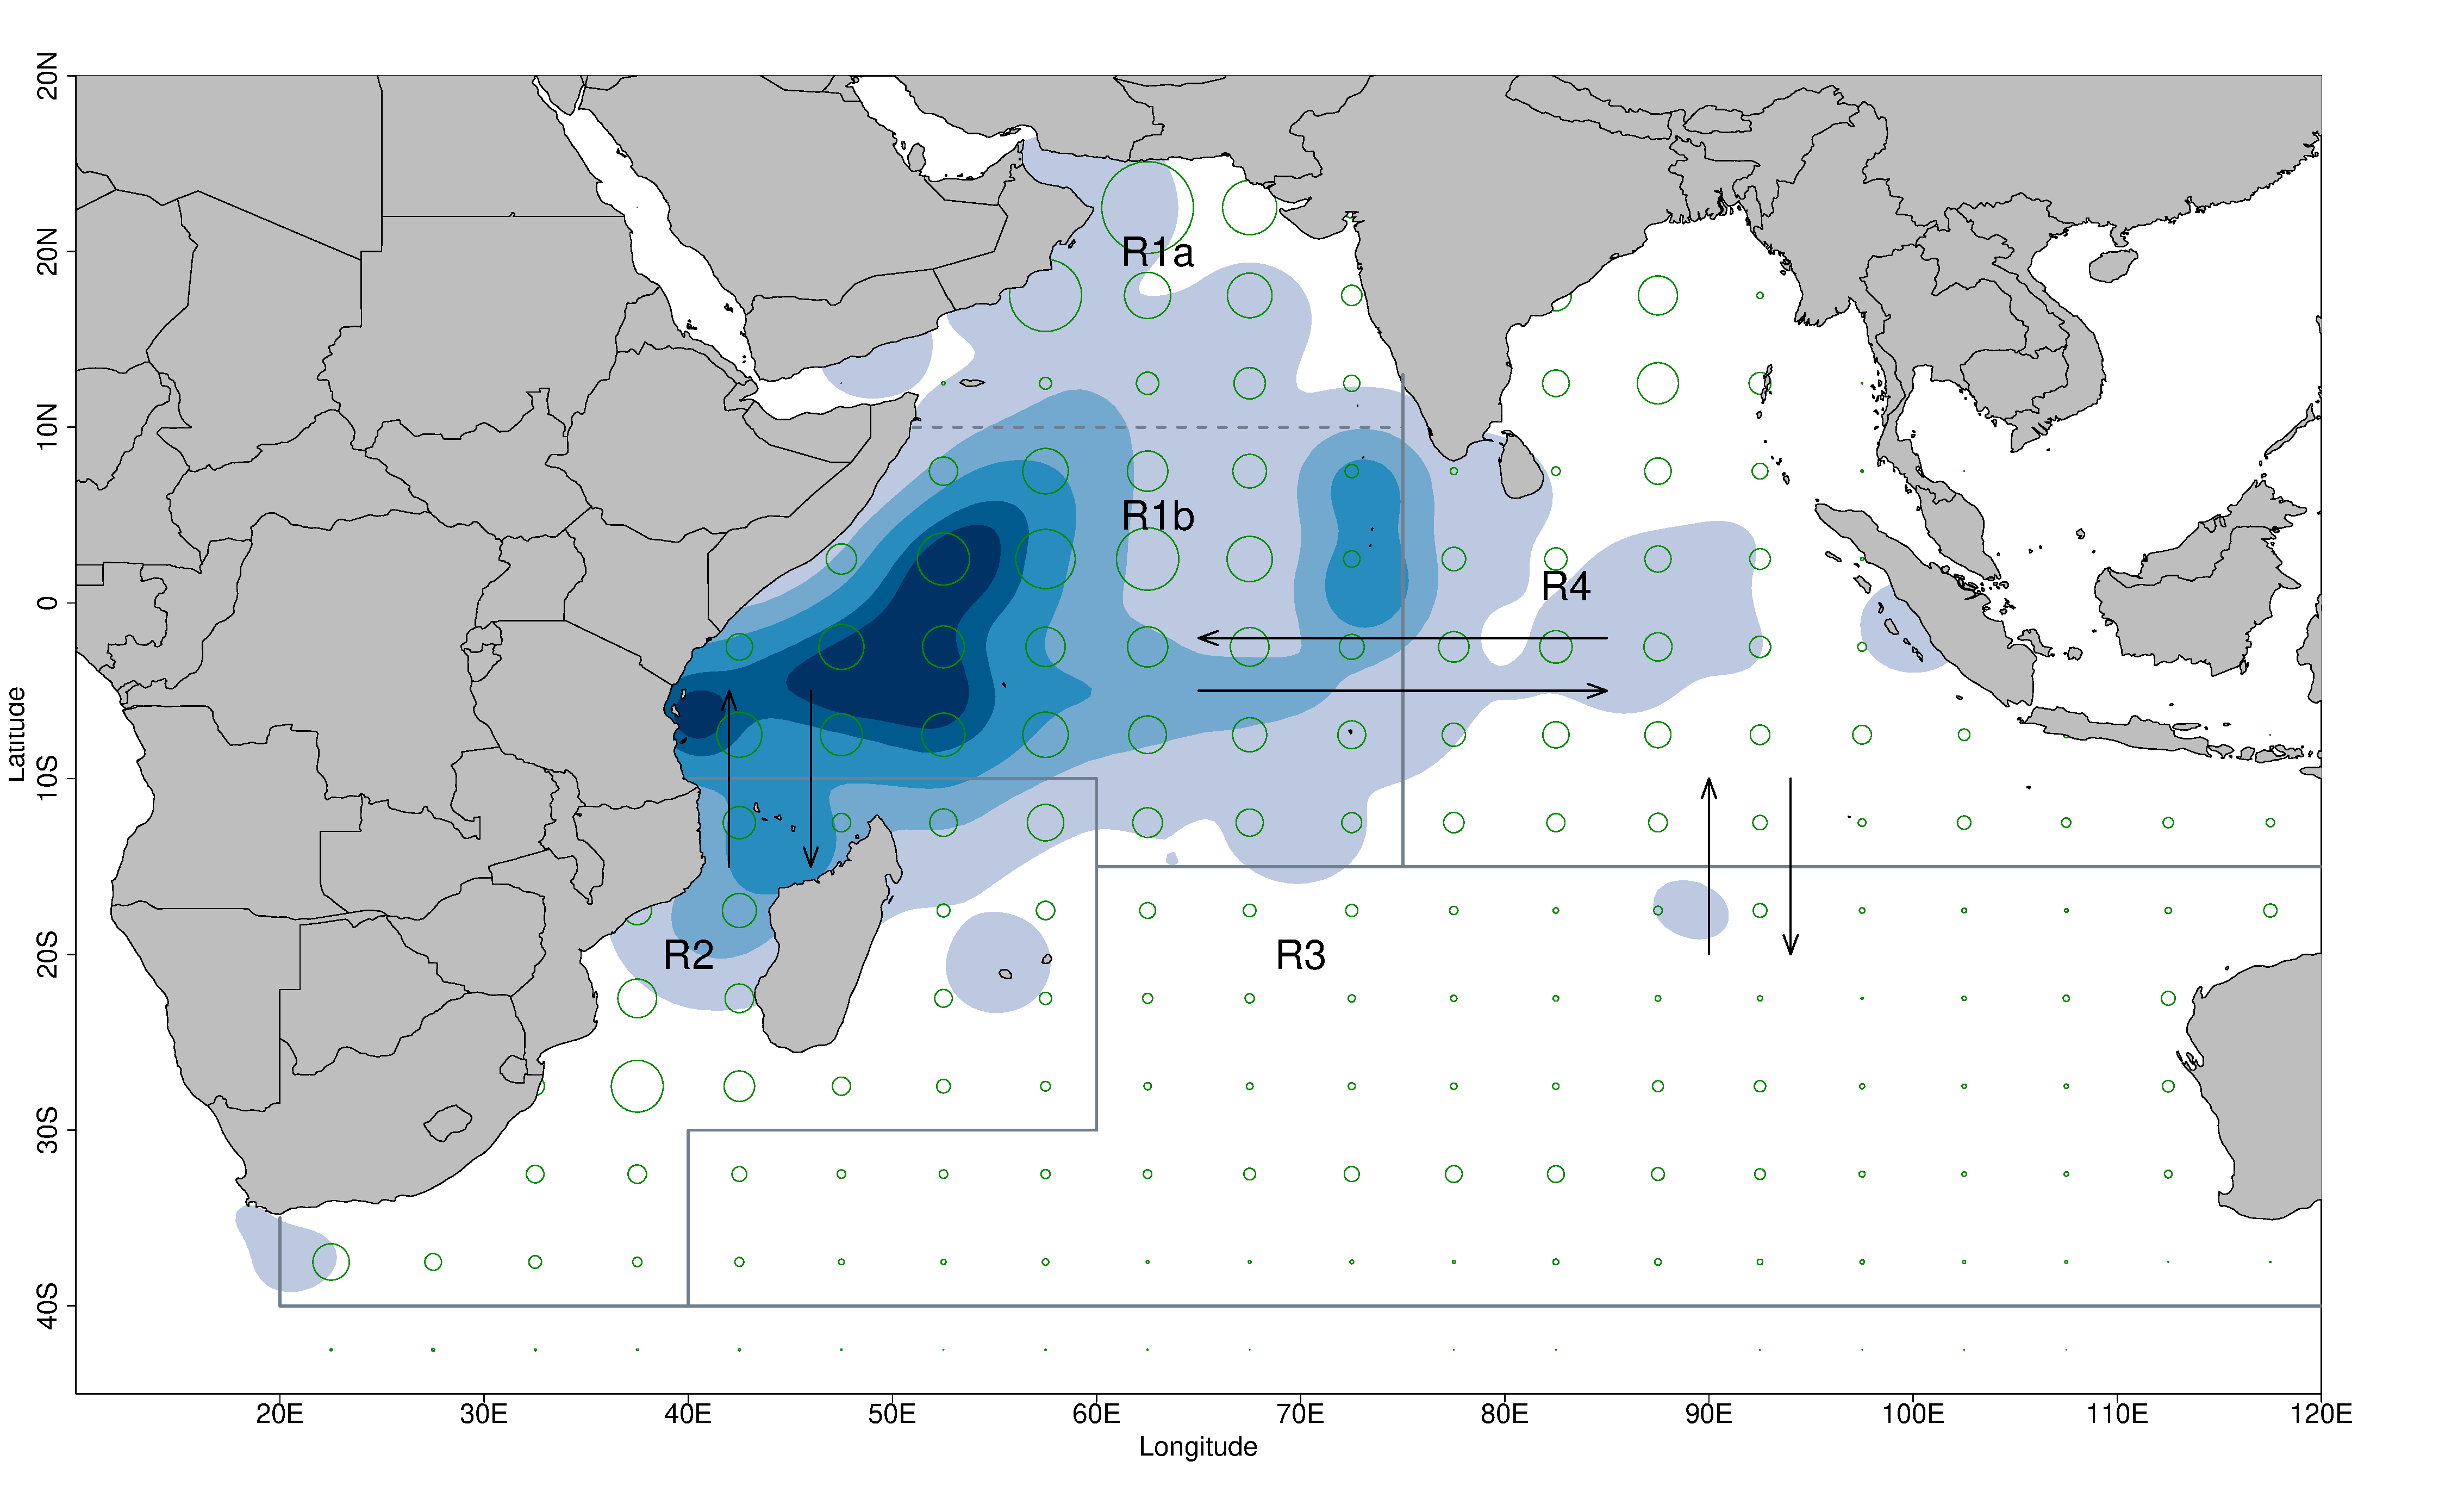
\includegraphics[width=6in]{fig1.eps}
\caption{Spatial stratification of the Indian Ocean for the four region assessment model (R1a and R1b were treated as a single model region R1, but were retained for the fleet definition). The black arrows represent the configuration of the movement parameterization.  Density contours represent of the dispersal of tag releases and subsequent recaptures from Indian Ocean Regional tuna tagging programme. Green circles represent the distribution of catches from the longline fishery aggregated by 5 degree longitude and latitude for 1980 to 2017 (max. = 133 770 t).}
\label{fig:map}
\end{figure*}


\begin{figure}
\centering
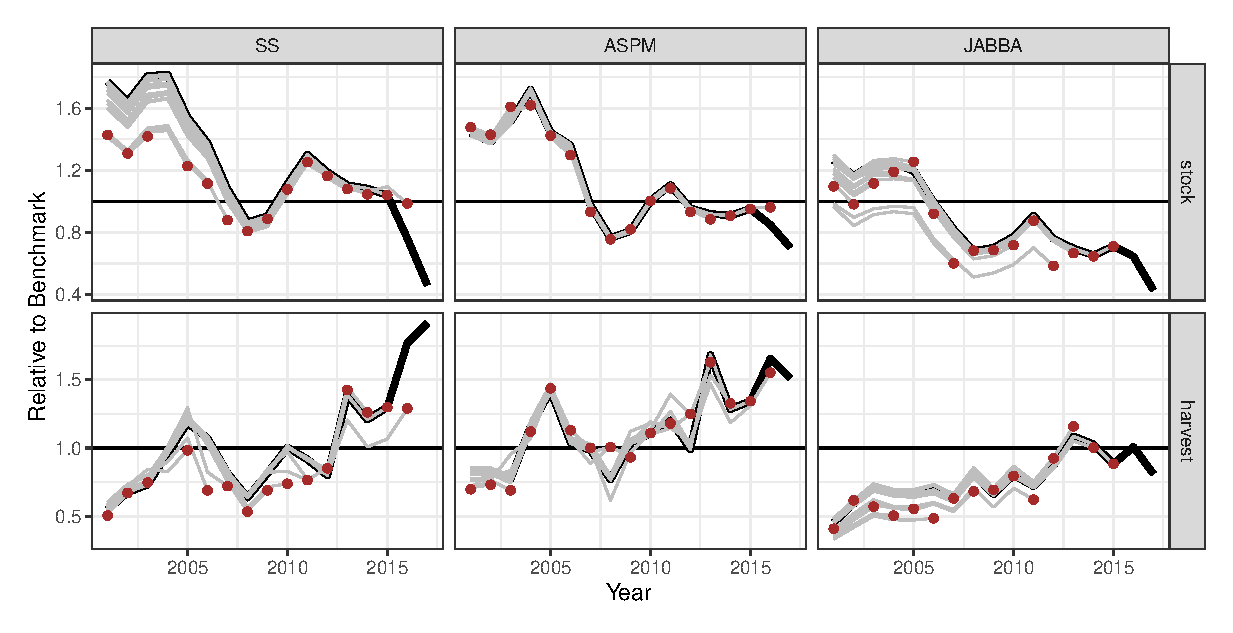
\includegraphics[width=6in]{fig2.eps}
\caption{Hindcasts for one-step ahead, the thick solid line represent the model estimates for $stock$ and $harvest$ relative to $MSY$ benchmarks, based on SSB and instantaneous fishing mortality for SS and ASPM-R and total biomass and harvest rate for JABBA. The points indicate the terminal years of the assessments peeled for the CPUE.}
\label{fig:retro}
\end{figure}


\begin{figure}
\centering
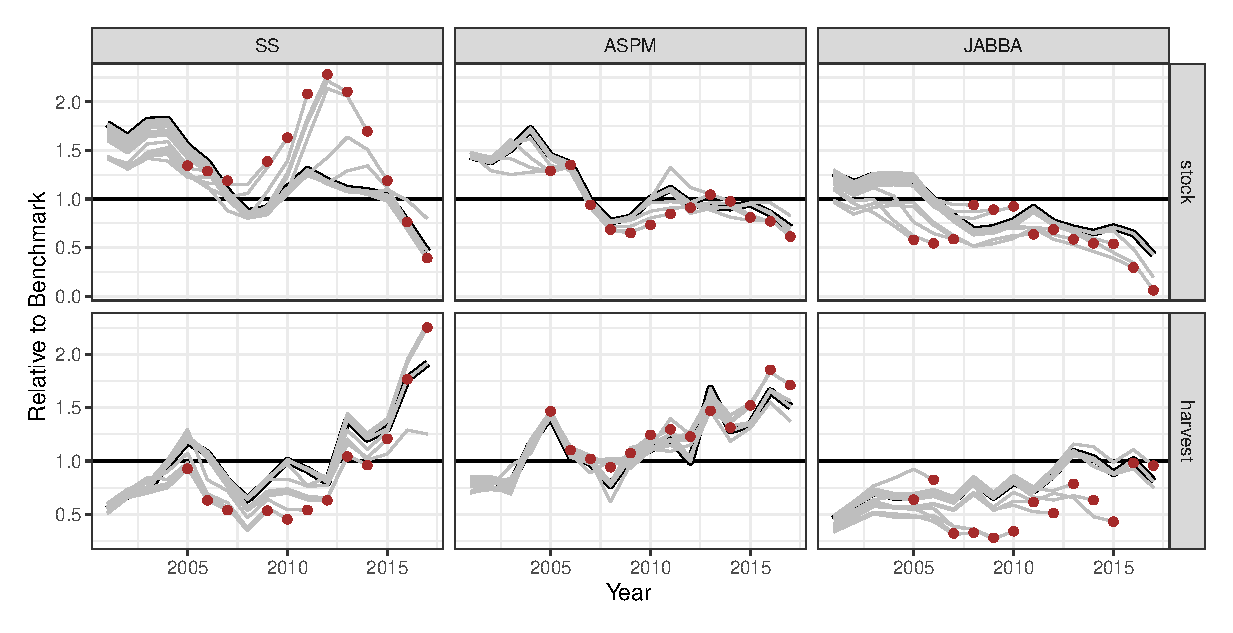
\includegraphics[width=6in]{fig3.eps}
\caption{Hindcasts for three-step ahead, the thick solid line represent the model estimates for $stock$ and $harvest$ relative to $MSY$ benchmarks, based on SSB and instantaneous fishing mortality for SS and ASPM-R and total biomass and harvest rate for JABBA. The points indicate the terminal years of the assessments peeled for the CPUE.}
\label{fig:retro3}
\end{figure}


\begin{figure*}[htbp]
\centering
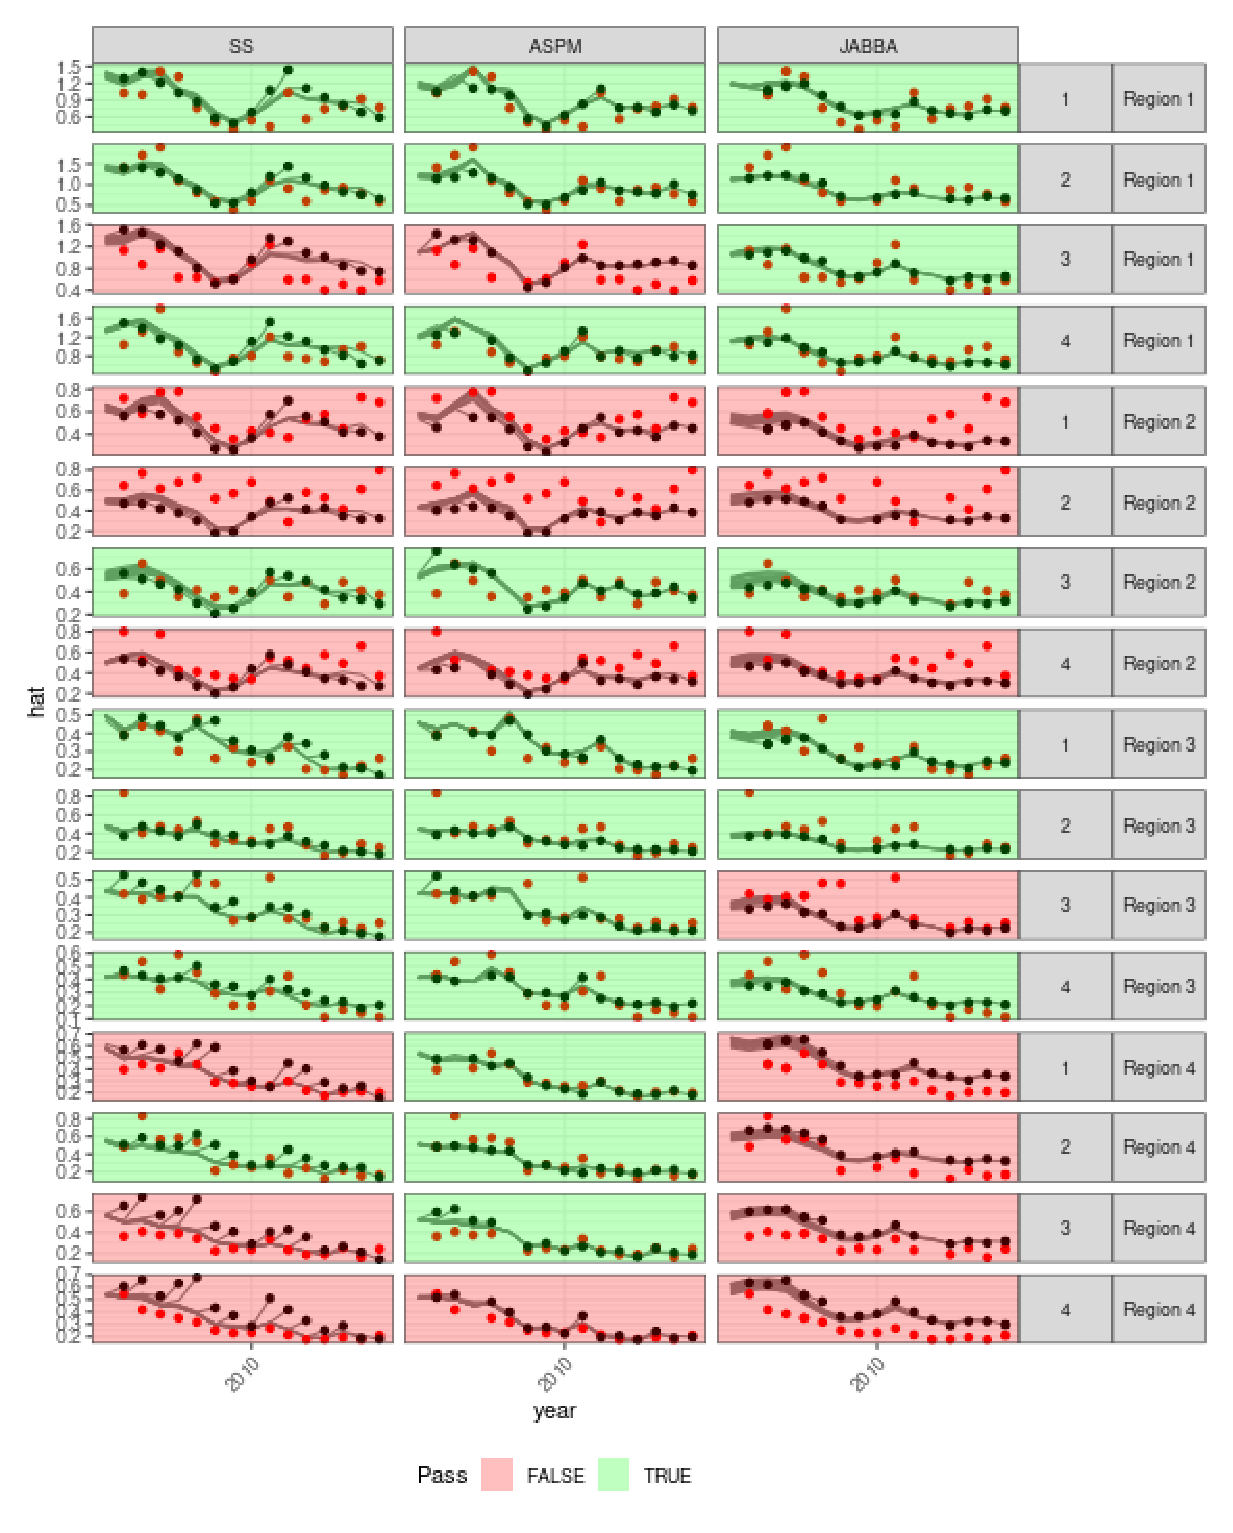
\includegraphics[width=6in]{fig4.eps}
\caption{Hindcasts with one-step ahead for CPUE indices by region and quarter. Green backgrounds indicate that the CPUE index passes Mean Absolute Scaled Error (MASE < 1) criterion, or failed (red) otherwise. Red dots are the observed CPUE values and thin lines are the fits with terminal hincast year indicated by a solid point.}
\label{fig:hy}
\end{figure*}

\begin{figure*}[htbp]
\centering
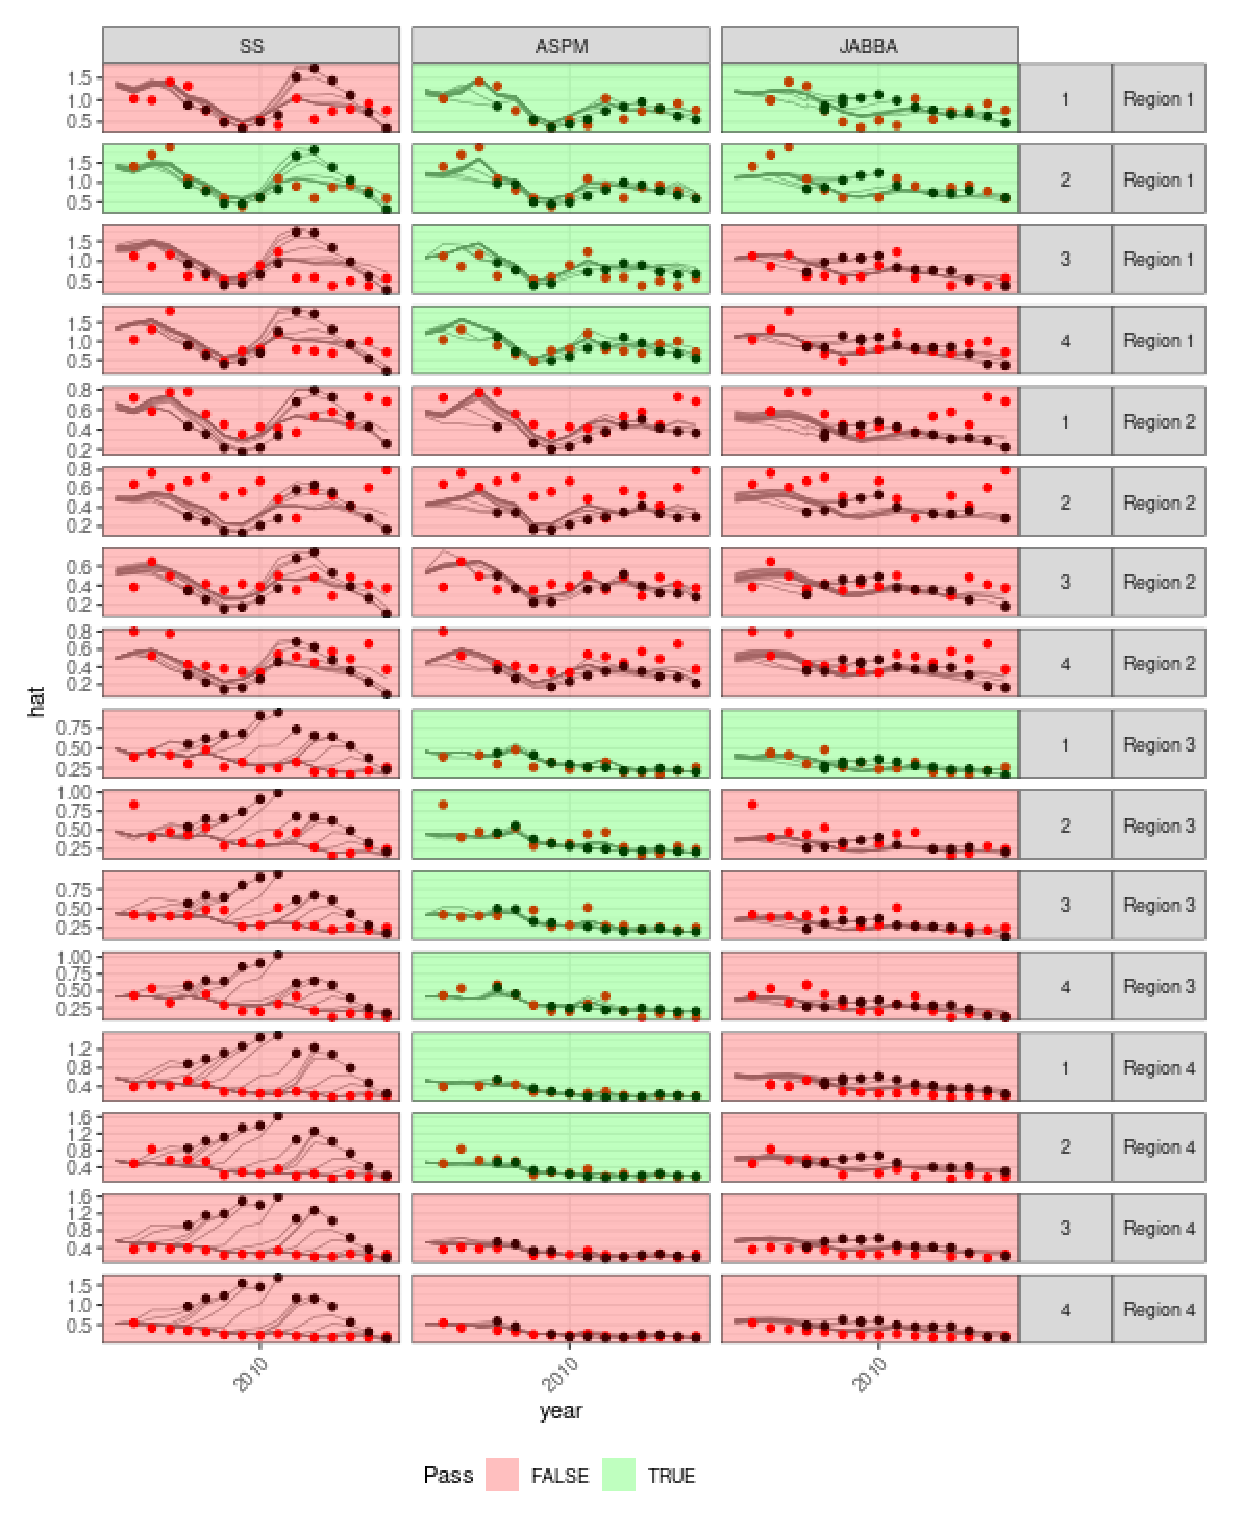
\includegraphics[width=6in]{fig5.eps}
\caption{Hindcasts for three-step ahead for CPUE indices by region and quarter. Green backgrounds indicate that the CPUE index passes Mean Absolute Scaled Error (MASE < 1) criterion, or failed (red) otherwise. Red dots are the observed CPUE values and thin lines are the fits with terminal hincast year indicated by a solid point.}
\label{fig:hy3}
\end{figure*}

\begin{figure*}[htbp]
\centering
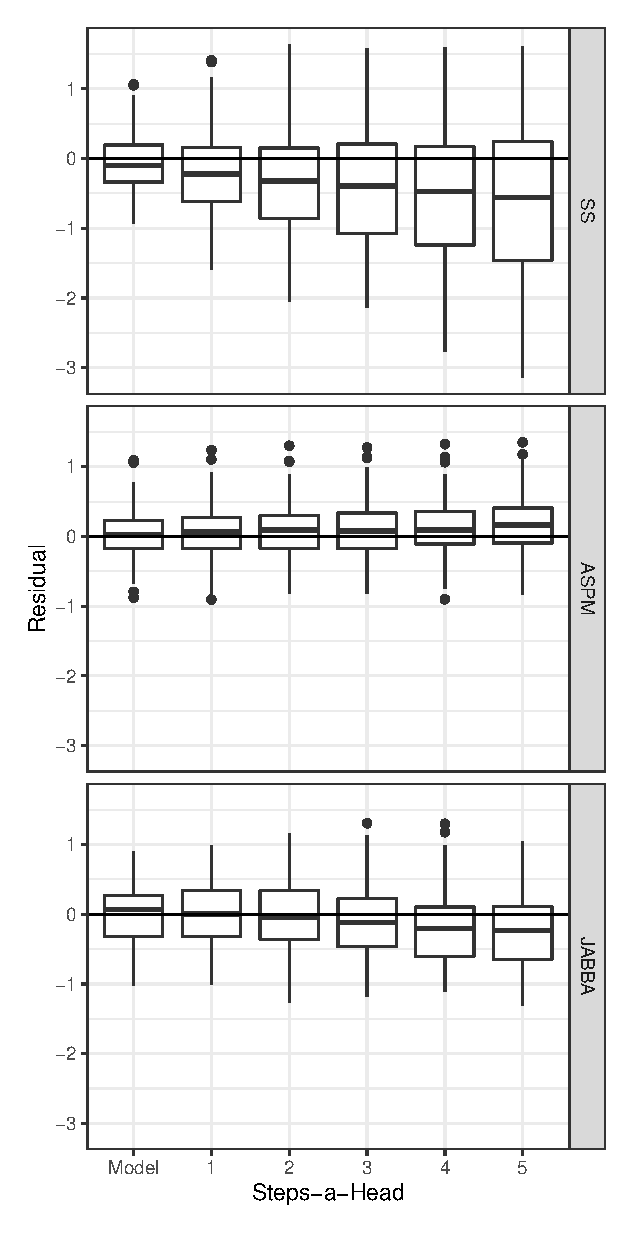
\includegraphics[width=4in]{fig6.eps}
\caption{Boxplots showing model residuals and prediction residuals for 1,2,3,4 and 5 year ahead projections, pooled for all CPUE indices across regions and quarters.}
\label{fig:residuals}
\end{figure*}

\end{document}